% !TEX TS-program = XeLaTeX
% !TeX program = xelatex

\documentclass{article}
\usepackage[slovak]{babel}
\usepackage[no-math]{fontspec}

\usepackage[top=2cm,left=2cm,bottom=2cm,right=2cm,a4paper]{geometry}
\usepackage{verbatim}                       % support for comment and verbatim
\usepackage{graphicx}                       % support for images
\usepackage{xcolor}							% support for colors
\usepackage[hidelinks]{hyperref}            % hyperlink support
\usepackage{etoolbox}                       % conditional statement support
\usepackage{tikz}
\usepackage{microtype}                      % stretchy line length
\usepackage{xfrac}                          % nice fractions for meters
\usepackage{wrapfig}                        % chords on page side
\usepackage{pbox}
\usepackage{tcolorbox}
\usepackage{fdsymbol}                       % nice arrows
\usepackage[usestackEOL]{stackengine}       % symbol stacking for plucking
\usepackage{relsize}                        % font size manipulation
\usepackage{incgraph}                       % cover image
\usepackage{tabularx}
\usepackage{environ}                        % define environments with body var
\usepackage[yyyymmdd]{datetime}
\usepackage{array}
\input{insbox}								% float for strumbox
\usepackage[stamp]{draftwatermark}			% disable: nostamp
\usepackage{framed}			% debug frames

% From https://tex.stackexchange.com/questions/318670/generating-ukulele-chord-diagrams

% Usage: \drawukulelechord[StartFret]{Label}{g,c,e,a}
% Where g,c,e,a are fret numbers, or -1 for a muted string.
\newcommand\drawukulelechord[3][1]{%
  \edef\startfret{#1}% default=1
  \edef\chordlabel{#2}%
  \edef\frets{#3}%
  \begin{tikzpicture}[
    x=2ex,
    y=2ex,
    line cap=butt,
    line width=.4pt,
    baseline=(current bounding box.center)
  ]
    \ifnum \startfret=1
      \draw[line width=1pt] (1,0) -- (4,0);
      \def\topy{0}
    \else
      \def\topy{0.5}
      \draw (1,0) -- (4,0);
      \node at (4.625,-0.5) {\smaller\smaller \startfret};
    \fi%
    \foreach \d in {1,...,4}{\draw (1,-\d) -- (4,-\d);}
    \foreach \d[count=\p] in \frets {
      \draw (\p,\topy) -- (\p,-4.5);
      \ifdefstring{\d}{-1}{
        \draw (\p,.25) +(-.125,-.125) -- +(.125,.125)
        +(-.125,.125) -- +(.125,-.125);
      }{
        \ifdefstring{\d}{0}{
          % \draw (\p,.25) circle(.125); % open string
        }{
          \fill (\p,.5-1*\d+\startfret-1) circle(.25);
        }
      }
    }
    \node at (2.5,-5.5) {\chordlabel};
    % \path[use as bounding box] (0.4,1.5) rectangle (4.6,-6.0);
    \path[use as bounding box] (0.4,1.0) rectangle (4.6,-6.0);
    % \draw (0.4,0.5) rectangle (4.6,-6.0);
    % \path[use as bounding box] (0.5,.5) rectangle (4.5,-5); % TODO: make larger now that I added the text?
  \end{tikzpicture}%
}
\makeatletter
\newcommand\defineukulelechord[3][\@nil]{%
  \csdef{@ukulelechord@#2}{%
    \def\chordlabel{#1}%
    \def\chordid{#2}%
    \def\frets{#3}%
    \ifx\chordlabel\@nnil
      \drawukulelechord{\chordid}{\frets}
    \else
      \drawukulelechord{\chordlabel}{\frets}
    \fi%
  }%
}
\newcommand\defineukulelechordfret[4]{%
  \csdef{@ukulelechord@#2}{%
    \def\chordlabel{#1}%
    \def\chordid{#2}%
    \def\startfret{#3}%
    \def\frets{#4}%
    \drawukulelechord[\startfret]{\chordlabel}{\frets}
  }%
}
\newcommand\ukulelechord[1]{%
  \ifcsdef{@ukulelechord@#1}{%
    \csuse{@ukulelechord@#1}%
  }{%
    \GenericError{}{Undefined ukulele chord '#1'}{}{}% 
  }%
  \ignorespaces
}
\makeatother

\newcommand{\ukechord}{\ukulelechord}

% Ab
\defineukulelechord{Ab}{5,3,4,3}

% A
\defineukulelechord{A}{2,1,0,0}
\defineukulelechord{Am}{2,0,0,0}
\defineukulelechord[Am]{Amalt}{2,0,0,3}
\defineukulelechord{Am7}{0,0,0,0}
\defineukulelechord{Am7b5}{2,3,3,3}
\defineukulelechord{Asus4}{2,2,0,0}
\defineukulelechord{A7}{0,1,0,0}
\defineukulelechord{A7sus4}{0,2,0,0}
\defineukulelechord{Am/C}{2,0,0,3}

% A#
\defineukulelechord[A\#m]{Asharpm}{3,1,1,1}

% Bb
\defineukulelechord{Bb}{3,2,1,1}
\defineukulelechord{Bb7}{1,2,1,1}
\defineukulelechord{Bbm7}{1,1,1,1}
% \defineukulelechordfret{Bb}{Bbfret5}{5}{7,5,6,5}

% B
\defineukulelechord{B7}{2,3,2,2}
\defineukulelechord{Bm}{4,2,2,2}
\defineukulelechord{Bm7}{2,2,2,2}
\defineukulelechord{Bdim}{1,2,1,2}

% C
\defineukulelechord{C}{0,0,0,3}
\defineukulelechord[C]{Cbarre3}{5,4,3,3}
\defineukulelechord{Csus4}{0,0,1,3}
\defineukulelechord{Caug}{1,0,0,3}
\defineukulelechord{C7}{0,0,0,1}
\defineukulelechord{C6}{0,0,0,0}
\defineukulelechord{Cadd9}{0,2,0,3}
\defineukulelechord{Cmaj7}{0,0,0,2}
\defineukulelechord{Cm}{0,3,3,3}
\defineukulelechord{Cm7}{3,3,3,3}
\defineukulelechord{Cm6}{2,3,3,3}  % Cm/A

% C#
\defineukulelechord[C\#]{Csharp}{1,1,1,4}
\defineukulelechordfret{C\#}{Csharpfret4}{4}{6,5,4,4}
\defineukulelechord[C\#dim]{Csharpdim}{0,1,0,1}

% D
\defineukulelechord{D}{2,2,2,0}
\defineukulelechord[D]{Dbarre2}{2,2,2,5}
\defineukulelechord{D7}{2,2,2,3}
\defineukulelechord{Dm}{2,2,1,0}
\defineukulelechordfret{Dm}{Dmfret5}{5}{7,5,5,5}
\defineukulelechord{Dm6}{2,2,1,2}
\defineukulelechord{Dm7}{2,2,1,3}
\defineukulelechord{Dsus2}{2,2,0,0}
\defineukulelechord{Dsus4}{2,2,3,0}
\defineukulelechord{Daug}{3,2,2,5}

% D#
\defineukulelechord[D\#dim]{Dsharpdim}{2,3,2,3}
\defineukulelechord[D\#m]{Dsharpm}{3,3,2,1}
\defineukulelechord[D\#m7]{Dsharpm7}{3,3,2,4}

% Eb
\defineukulelechord{Eb}{0,3,3,1}

% E
\defineukulelechord{E}{4,4,4,2}
\defineukulelechord{Em}{0,4,3,2}
\defineukulelechord{Em7}{0,2,0,2}
\defineukulelechord{E6}{4,4,4,4}
\defineukulelechord{E7}{1,2,0,2}
\defineukulelechord{E7sus4}{2,2,0,2}
\defineukulelechord{Edim}{0,1,0,1}

% F
\defineukulelechord{F}{2,0,1,0}
\defineukulelechordfret{F}{Ffret5}{5}{5,5,5,8}
\defineukulelechord{F7}{2,3,1,0}
\defineukulelechord[F7]{F7alt}{2,3,1,3}
\defineukulelechordfret{Fmaj7}{Fmaj7fret5}{5}{5,5,5,7}
\defineukulelechordfret{F6}{F6}{5}{5,5,5,5}
\defineukulelechord{Fm}{1,0,1,3}
\defineukulelechord{Fdim}{1,2,1,2}
\defineukulelechord{Fadd2}{0,0,1,0}
\defineukulelechord{F/C}{2,0,1,3}

% F#
\defineukulelechord[F\#]{Fsharp}{3,1,2,1}
\defineukulelechord[F\#m]{Fsharpm}{2,1,2,0}
\defineukulelechord[F\#dim]{Fsharpdim}{2,3,2,3}


% G
\defineukulelechord{G}{0,2,3,2}
\defineukulelechord[G]{Gbarre2}{4,2,3,2}
\defineukulelechord{G5}{0,2,3,5}
\defineukulelechord{G7}{0,2,1,2}
\defineukulelechord{Gm}{0,2,3,1}
\defineukulelechord{Gm7}{0,2,1,1}
\defineukulelechord{Gm6}{0,2,0,1}
\defineukulelechord{Gmmaj7}{0,2,2,1}
\defineukulelechord{Gsus2}{0,2,3,0}

% G#
\defineukulelechord[G\#dim]{Gsharpdim}{1,2,1,2}


% Font
\setmainfont{Verdana}

% Enable centered table cells with specified width
\newcommand{\PreserveBackslash}[1]{\let\temp=\\#1\let\\=\temp}
\newcolumntype{C}[1]{>{\PreserveBackslash\centering}p{#1}}
\newcolumntype{R}[1]{>{\PreserveBackslash\raggedleft}p{#1}}
\newcolumntype{L}[1]{>{\PreserveBackslash\raggedright}p{#1}}

%%%%%%%%%%%%%%%%%%%%%%%%%%%%%%%%%%%%%%%%%%
% SONG

% Song environment
\newenvironment{song}{%
	\pagebreak%
	\parindent0pt%
	\normalsize%
}{%
}%

% Song header.
% Params: title, author, [title size - default \huge]
\newcommand{\SongTitle}[3][\huge]{%
	\phantomsection%
	\addcontentsline{toc}{subsection}{#2\ \ \textit{(#3)}}%
	{\centering
		#1 \textbf{#2} \penalty-1{\Large (#3)}\par
		\vspace{0.75ex}
	}
}

% Headerbox.
\NewEnviron{headerbox}{{\it\centering\BODY\par\vspace{0.5ex}}}%
\newcommand{\RaiseBoxWithAccents}{\vspace{-1.6ex}}
\newcommand{\RaiseBoxWithChucks}{\vspace{-1ex}}

% Chordbox environment. Places chords in a float at the right side of the page.
\newenvironment{vchordbox}{%
	\wrapfloat{minipage}{r}{7.5ex}%
	\vspace{-3ex}%
}{%
	\vspace{-12ex}% Get rid of a mysterious white space at the bottom
	\endwrapfloat%
}%
\NewEnviron{hchordbox}{{\centering\BODY\par}\vspace{0.5ex}}%

% Strumbox.
\NewEnviron{strumbox}{%
    \InsertBoxR{0}{{\vrule height 2.5ex depth 0pt width 0pt}\BODY}%
}%

% Chorusbox environment. Makes a box around text, used mostly for choruses.
% Takes one parameter, the text displayed at the top of the box.
\newsavebox{\chbox}
\newlength{\chboxsep}
\setlength{\chboxsep}{1.5ex}
\newlength{\savedfboxsep}
\newenvironment{chorusbox}[1]{%
	\hspace{-\chboxsep}%
	\begin{lrbox}{\chbox}%
		\begin{minipage}{\linewidth-3ex}%
			#1\textbf{:} \par \smallskip
		}{%
		\end{minipage}%
	\end{lrbox}%
	\setlength{\savedfboxsep}{\fboxsep}%
	\setlength{\fboxsep}{\chboxsep}%
	\fbox{\usebox{\chbox}}%
	\setlength{\fboxsep}{\savedfboxsep}%
}
\newenvironment{chorusboxwide}[1]{%
	\hspace{-\chboxsep}%
	\begin{lrbox}{\chbox}%
		\begin{minipage}{\linewidth}%
			#1\textbf{:} \par \smallskip
		}{%
		\end{minipage}%
	\end{lrbox}%
	\setlength{\savedfboxsep}{\fboxsep}%
	\setlength{\fboxsep}{\chboxsep}%
	\fbox{\usebox{\chbox}}%
	\setlength{\fboxsep}{\savedfboxsep}%
}%

% Remarks
\newcommand{\instruction}[1]{\textbf{\smaller\textit{[#1]}}\vspace{0.2ex}}
\newcommand{\vocals}[1]{\textit{(#1)}}

% Chord macros
\newcommand{\ch}[1]{\textbf{(#1)}}
\newcommand{\rep}[1]{\hspace{2pt}x#1}
\newcommand{\early}{*}
\newcommand{\beatsymbol}{\textquotesingle}
\newcount\myloopcounter
\newcommand{\beats}[1]{%
  \myloopcounter0% initialize the loop counter
  \loop\ifnum\myloopcounter < #1 % Test if the loop counter is < #1
  \beatsymbol% <<<< the thing to repeat
  \advance\myloopcounter by 1 % 
  \repeat % start again
}
\newcommand{\beat}{\beats1}
%\newcommand{\beatsperchord}[1]{(X) = (X\beats#1)}
\newcommand{\beatsperchord}[1]{(X) = #1 beats}
\newcommand{\suptriangle}{$^\triangle$}


% Tags
\newcommand{\Refren}{\textbf{R{\smaller EFRÉN}}}
\newcommand{\Chorus}{\textbf{C{\smaller HORUS}}}
\newcommand{\Intro}{\textbf{I{\smaller NTRO}:\ }}
\newcommand{\Outro}{\textbf{O{\smaller UTRO}:\ }}
\newcommand{\Prechorus}{\textbf{P{\smaller RE-CHORUS}}}
\newcommand{\PrechorusAndChorus}{\textbf{P{\smaller RE-CHORUS AND} C{\smaller HORUS}}}
\newcommand{\PredrefrenARefren}{\textbf{P{\smaller REDREFRÉN A} R{\smaller EFRÉN}}}
\newcommand{\Bridge}{\textbf{B{\smaller RIDGE}}}
\newcommand{\Instrumental}{\textbf{I{\smaller NSTRUMENTAL}}}

%%%%%%%%%%%%%%%%%%%%%%%%%%%%%%%%%%%%%%%%%%
% STRUMMING

\newcommand{\fixwidth}[2][7pt]{\hbox to#1{\hss$#2$\hss}}
\newcommand{\rang}{\begin{picture}(5,7)
\put(1.1,2.5){\rotatebox{135}{\line(1,0){3.0}}}
\put(1.1,2.5){\rotatebox{225}{\line(1,0){3.0}}}
\end{picture}}
\newcommand{\Miss}{\fixwidth\cdot}
\newcommand{\Down}{\fixwidth\downarrow}
\newcommand{\AccentDown}{\fixwidth{\stackrel{\rang}{\downarrow}}}
\newcommand{\ChuckDown}{\fixwidth{\stackrel{\scriptscriptstyle\times}{\downarrow}}}
\newcommand{\StaccatoDown}{\fixwidth{\stackrel{\cdot}{\downarrow}}}
\newcommand{\Up}{\fixwidth\uparrow}
\newcommand{\AccentUp}{\fixwidth{\stackrel{\rang}{\uparrow}}}
\newcommand{\ChuckUp}{\fixwidth{\stackrel{\scriptscriptstyle\times}{\uparrow}}}
\newcommand{\StaccatoUp}{\fixwidth{\stackrel{\cdot}{\uparrow}}}
\newcommand{\Separator}{\hspace{3pt}\big|\hspace{3pt}}
% Example usage: \PluckDown{A E G}
\newcommand{\PluckDown}[1]{\fixwidth{\stackrel{\scalebox{0.5}{\shortstack{#1}}}{\downarrow}}}
\newcommand{\PluckUp}[1]{\fixwidth{\stackrel{\scalebox{0.5}{\shortstack{#1}}}{\uparrow}}}


%%%%%%%%%%%%%%%%%%%%%%%%%%%%%%%%%%%%%%%%%%
% VERSION
\renewcommand{\dateseparator}{-}
\newcommand{\songbookversion}{v0.6.\today}
\SetWatermarkText{Beta \songbookversion}
\SetWatermarkColor[gray]{0.5}
\SetWatermarkFontSize{0.4cm}
\SetWatermarkAngle{90}
\SetWatermarkHorCenter{0.5cm}


\begin{document}%

% Dark mode
%\pagecolor[rgb]{0,0,0} %black
%\color[rgb]{0.7,0.7,0.7} %grey
%\color[rgb]{0.7,0.5,0.0} %orange
\incgraph{cover.png}

\begin{titlepage}
	\begin{center}
		\vspace*{1cm}

		\vspace{6cm}

		
\includegraphics[width=0.5\textwidth]{title.png}

		\vspace{6cm}

		\it
		\LARGE
		www.ukulelespevnik.sk

		\vspace{1cm}

		\Large
		Beta \songbookversion

	\end{center}
\end{titlepage}

% Table of contents.
\tableofcontents

\newpage
% Adjust formatting.
\begingroup % Original formatting is reset back with \endgroup
\setlength{\parindent}{0pt}
\setlength{\parskip}{\baselineskip}
\large

\section*{Úvod}

Všetkých Vás vítam v Citrónovom ukulele spevníku! Či už hráte na ukulele alebo iný nástroj,
a či ste začiatočníci alebo pokročilí, dúfam, že si v spevníku nájdete niečo pre Vás.

Tento spevník vznikol hlavne z dvoch dôvodov. Prvým je krátkodobá pamäť. U nás sa v spevníkoch
zvyknú uvádzať akordy iba v prvej slohe a v ostaných si ich treba buď pamätať alebo skákať očami
hore-dole, čo mne nikdy nešlo. Tu sú akordy uvedené všade.

Druhý dôvod sú piesne, ktoré poznám iba približne. Možno sa Vám už stalo, že zistíte, že neviete
ako presne vybranú pieseň zahrať, pretože vlastne poznáte len jej refrén alebo časť slohy.
Alebo sprevádzate niekoho, kto ju pozná, akurát by ste potrebovali vedieť, kedy zmeniť akord.
V tomto spevníku je preto naznačené, ako dlho akordy hrať.

A keďže hrám na ukulele, tak vznikol ukulele spevník.\footnote{Spevník bol inšpirovaný Londýnskym
spevníkom Ukulele Wednesdays. Odporúčam :)} Akordy sú miestami prispôsobé tak, aby sa dobre hrali
na tomto malebnom nástroji, ale spevník je použiteľný aj pre napríklad gitaru. Tiež dúfam,
že takto môžem prispieť k formujúcej sa ukulele komunite na Slovensku.

V neposlednom rade, uživajte si radosť z hrania! Neexistuje nič také ako \uv{ako sa pesnička má hrať
správne}, je na každom interpretovi, ako si ju prispôsobí, aby sa mu páčila. Ja som sa snažil
akordy uvádzať blízko originálu, ale nakoľko je to veľmi rozsiahly projekt, určite sú v spevníku chyby.
(Akordy, text, časovanie.) Pokiaľ na nejakú narazíte, alebo by ste chceli do spevníku prispieť, dajte
mi určite vedieť! [TODO: Štylistika.]

Z lockdownu v Londýne,

\textit{%
Mišo \\
Január 2021
}

\section*{Použité značky}

\subsection*{Akordy}

V spevníku používame anglické značenie, ktoré je bežné u zahraničných piesní. Zápis \textbf{B, Bb}
preto označuje noty \textbf{H, B} v nemeckom značení, ktoré sa učí u nás.

Hudobný zápis je organizovaný do \textbf{taktov.} Každý takt pozostáva z niekoľkých
\textbf{dôb.} V spevníku značka \ch{C} značí akord, ktorý trvá celý takt, \ch{C\beats2}
značí akord trvajúci toľko dôb, koľko je čiarok. Na začiatku piesne je uvedené zápisom \beatsperchord{2},
koľko dôb má jeden takt. Keďže väčšina piesní sa hrá na štyri doby, predpis \beatsperchord{4} vynechávame.

Text obsahuje diagramy akordov pre štandardné ukulele ladenie GCEA. Pre úsporu miesta sú niekedy
vynechané nasledujúce štyri základné akordy:
\begin{center}
\smaller
\ukechord{C}
\ukechord{G}
\ukechord{F}
\ukechord{Am}
\larger
\end{center}

Na rozdiel od ostatných spevníkov sú akordy uvedené priamo v texte, text sa tak lepšie zmestí
na stránku. Pokiaľ medzi akordom a textom \textbf{nie je medzera,} slová textu sa začínajú spievať
naraz s akordom, s medzerou sa text začína spievať neskôr.\footnote{Minimálne taká bola snaha :)}

\textit{%
Poznámka pre pokročilých: Pretože ukulele nemá basové struny, akordy s lomítkom sa všeobecne
nepoužívajú. Základný tón akordu preto nemusí byť rovnaký ako čo má hrať basgitara. Napríklad
(C/B) alebo (D/A) môžu byť prepísané ako (Cmaj7) alebo (D).
}

\medskip

\begin{tabularx}{\linewidth}{ l X }
    \ch{C\beats2} & Hraj akord toľko dôb koľko je čiarok \\ 
    \ch{C} & Hraj akord na dĺžku jedného taktu \\
    \ch{C\rep2} & Hraj akord na dĺžku viacerých taktov \\
    \ch{*C} & Skráť predošlý akord a predĺž tento o dobu alebo poldoby (podľa piesne)\footnote{%
    Napríklad \ch{D} \ch{*G} môže byť realizované ako \ch{D\beats3}\ch{G\beats5}.} \\
    \ch{C-G-C} & Skratka pre hranie akordov aby sa zmestili do jedného taktu \\
    \ch{N.C.} & Hudobná pauza, z anglického \textit{no chord}
\end{tabularx}


\subsection*{Rytmický sprievod}

Rukou, ktorá nedrží akord, hráme \textbf{rytmický sprievod,} v angličtine popisnejšie nazvaný
\emph{strumming pattern}. Na každú dobu robí ruka pohyb dole a hore. Napríklad pre štvordobový
takt počítame:
{\larger$$
\PluckDown{Pr}\ \PluckUp{vá}\ \PluckDown{Dru}\ \PluckUp{há}\ 
\PluckDown{Tre}\ \PluckUp{tia}\ \PluckDown{Štvr}\ \PluckUp{tá}\ 
$$}%
Sprievod je tvorený tým, pri ktorých pohyboch (ne)udierame struny, kde dáme prízvuk a podobne.

Na vrchu stránky uvádzame príklad rytmického sprievodu, viď značky v tabuľke nižšie.
Ten by mal slúžiť iba ako inšpirácia, sprievod do istej miery simuluje bicie a je na každom, ako ich
interpretovať. Sprievod nie je uvedený pri piesniach, kde sa hrá \uv{štandardný} sprievod (pozri nižsie)
alebo kde nebolo jasné, aký zvoliť.

V sprievodoch s prízvukom sa niektoré neprízvučné údery nadol zvyknú hrať iba ako ľahký dotyk
struny G. Tento štýl dáva vyznieť ladeniu struny G a dotvára charakteristický zvuk ukulele.
Nie je pevné pravidlo, ktoré údery sa majú takto hrať, častokrát to ale býva neprízvučná doba pred
prízvukom.

Označenie \textbf{swing} znamená, že pohyb rukou dole trvá dlhšie ako pohyb hore -- približne
dve tretiny doby vs. tretina doby. Swingový rytmus sa hrá veľmi bežne, označenie možno pri
niektorých piesniach chýba (dajte mi vedieť). [TOTO: swing ako default?]

Jeden pohyb ruky dole a hore väčšinou zaberá jednu dobu. Označenie \textbf{double time} znamená,
že sa sprievod hrá dvakrát rýchlešie, t.j. na pol doby. Naopak, \textbf{half time} značí dvakrát
pomalšie hranie, t.j. na dve doby.

\medskip

\def\mystrut{\vrule height 18pt depth 0pt width 0pt}
\begin{tabularx}{\linewidth}{ c X }
    \mystrut $\Down\Up$ & Úder cez všetky struny dole/hore \\ 
    \mystrut $\Separator$ & Oddeľuje logické celky sprievodu, napr. zmenu akordu \\ 
    \mystrut $\AccentDown$ & Prízvuk \\  
    \mystrut $\StaccatoDown$ & Staccato, stlm struny ihneď po údere \\
    \mystrut $\ChuckDown$ & Tlmený úder, anglicky \textit{chuck} \\
    \mystrut $\PluckDown{R}$ & Rasgueado, \uv{vejárovitý} úder cez všetky struny viacerými prstami \\    
    \mystrut $\PluckDown{E A}$ & Brnkni iba struny uvedené nad akordom. Na smere šípky nezáleží. \\
\end{tabularx}


\subsection*{Niektoré základné sprievody}

\begin{tabularx}{\linewidth}{ l X }
    \mystrut $\Down\Miss\Down\Miss\Down\Miss\Down\Miss$ & 
    Jednoduchý sprievod vhodný pre začiatočíkov, ktorý často funguje prekvapivo dobre.
    Hraj úder dole na každú dobu. \\ 

    \mystrut $\Down\Miss\Down\Up\Miss\Up\Down\Up$ &
    Najrozšírenejší, \uv{štandardný} sprievod ktorý je vhodný k väčšine piesní. Nemá ustálený názov,
    po anglicky sa používajú označenia \textit{common, island, Calypso, d-du-udu} alebo
    \textit{Old faithful strum}. Bežne sa hrá so swingom. Dve populárne variácie s prízvukom:
    $\AccentDown\Miss\Down\AccentUp\Miss\Up\AccentDown\Up$ a
    $\Down\Miss\AccentDown\Up\Miss\Up\AccentDown\Up$ \\ 

    \mystrut $\Down\Miss\AccentDown\Up\ \Down\Miss\AccentDown\Up$ & Tento sprievod znie
    skvelo na ukulele. Pri úderoch pred prízvukom sa iba zľahka dotknite G struny, akoby ste hrali:
    $\PluckDown{G}\Miss\AccentDown\Up\ \PluckDown{G}\Miss\AccentDown\Up$ \\  
\end{tabularx}


\subsection*{FAQ}

\textbf{Q: Hrám na gitaru. Môžem spevník použivať ako gitarový spevník?}

Áno, určite! V 99\% prípadov sa hrajú rovnaké akordy na gitare. Niektoré pesničky boli transponované
aby sa hrali dobre na ukulele, odporúčam naučiť sa akord \ch{Eb} (ako \ch{C} s barre na treťom pražci).
Tiež si niekedy treba dať pozor na akordy s lomítkom, keďže ukulele nemá basové struny, napríklad namiesto
\ch{C/B} sa na ukulele zvykne hrať \ch{Cmaj7}.

\textbf{Q: Niektoré akordy vyzerajú zložito. Čo mám robiť?}

Akordy sa dajú zjednodušiť. Väčina akordov je odvodených buď z durového alebo mollového akordu,
takže namiesto \ch{Cmaj7} alebo \ch{Gm6} sa dá hrať \ch{C} alebo \ch{Gm}. Akord \ch{E}, ktorý
sa ťažko chytá, sa dá nahradiť \ch{E7}. A napokon niektoré akordy ako \textbf{dim} a \textbf{sus}
sa často dajú vynechať.

\textbf{Q: Prečo citrónový?}

Pretože také je pozadie na obálke.


\subsection*{Acknowledgements}

Olin :)

\endgroup

% Songs.
\newgeometry{top=1.5cm,left=1cm,bottom=1.5cm,right=1cm,footskip=0.75cm}
% % THIS FILE IS AUTOGENERATED.
% DO NOT EDIT!
\begin{song}

\SongTitle{All My Loving}{The Beatles}

\begin{headerbox}
\RaiseBoxWithAccents
\textit{Original: +4} \quad
\textit{Strum:} $\Down\Miss\AccentDown\Up\Miss\Up\AccentDown\Up$
\end{headerbox}

\begin{hchordbox}
\ukechord{Am}
\ukechord{Am/C}
\ukechord{Bb}
\ukechord{C}
\ukechord{Caug}
\ukechord{Dm}
\ukechord{F}
\ukechord{G7}
\end{hchordbox}

\large

\bigskip

Close your \ch{Dm}eyes and I'll \ch{G7}kiss you, to\ch{C}morrow I'll \ch{Am}miss you \par
Re\ch{F}member I'll \ch{Dm}always be \ch{Bb}true \ch{G7} \par
And then \ch{Dm}while I'm a\ch{G7}way I'll write \ch{C}home every\ch{Am}day \par
And I'll \ch{F}send all my \ch{G7}loving to \ch{C\rep2}you \par

\bigskip

I'll pre\ch{Dm}tend that I'm \ch{G7}kissing the \ch{C}lips I am \ch{Am}missing \par
And \ch{F}hope that my \ch{Dm}dreams will come \ch{Bb}true \ch{G7} \par
And then \ch{Dm}while I'm a\ch{G7}way I'll write \ch{C}home every\ch{Am}day \par
And I'll \ch{F}send all my \ch{G7}loving to \ch{C\rep2}you \par

\bigskip

All my \ch{Am/C}loving \ch{Caug}I will send to \ch{C\rep2}you \par
All my \ch{Am/C}loving, \ch{Caug}darling, I'll be \ch{C\rep2}true \par

\bigskip

Close your \ch{Dm}eyes and I'll \ch{G7}kiss you, to\ch{C}morrow I'll \ch{Am}miss you \par
Re\ch{F}member I'll \ch{Dm}always be \ch{Bb}true \ch{G7} \par
And then \ch{Dm}while I'm a\ch{G7}way I'll write \ch{C}home every\ch{Am}day \par
And I'll \ch{F}send all my \ch{G7}loving to \ch{C\rep2}you \par

\bigskip

All my \ch{Am/C}loving \ch{Caug}I will send to \ch{C\rep2}you \par
All my \ch{Am/C}loving, \ch{Caug}darling, I'll be \ch{C\rep2}true \par

\bigskip

All my \ch{Am/C\rep2}loving… A-a-all my \ch{C\rep2}loving o-oh \par
All my \ch{Am/C\rep2}loving… I will send to \ch{C\rep2}you  \par

\end{song}

\begin{song}

\SongTitle{American Pie}{Don McLean, abridged}

\begin{headerbox}
\textit{Verse:} $\Down\Miss\Down\Up\Miss\Up\Down\Up$ \quad
\textit{Chorus:} $\Down\Miss\Down\Up \Separator \Down\Miss\Down\Up \Separator \Down\Up\Down \Separator \Up\Miss\Up\Down\Up$ \quad
\end{headerbox}

\begin{chordbox}
% \ukechord{G} \par
\ukechord{D} \par
\ukechord{Em7} \par
% \ukechord{Am} \par
% \ukechord{C} \par
\ukechord{Em} \par
\ukechord{D7} \par
\ukechord{A7} \par
\end{chordbox}

\normalsize

\bigskip

\note{single strums, slowly} \par
A \ch{G\beats2}long, \ch{D\beats2}long \ch{Em7}time ago \ch{Am} I can still re\ch{C}member \par
How that \ch{Em}music used to \ch{D\rep2}make me smile \par
And \ch{G\beats2}I knew \ch{D\beats2}if I \ch{Em7}had my chance that \ch{Am}I could make those \ch{C}people dance \par
And \ch{Em}maybe they'd be \ch{C}happy for a \ch{D\rep2}while \par

\bigskip

But \ch{Em}February \ch{Am}made me shiver, with \ch{Em}every paper \ch{Am}I'd deliver \par
\ch{C\beats2}Bad news \ch{G\beats2}on the \ch{Am}doorstep, I \ch{C}couldn't take one more \ch{D}step \par
I \ch{G\beats2}can't re\ch{D\beats2}member \ch{Em}if I cried when I \ch{Am}read about his \ch{D}widowed bride \par
\ch{G\beats2}Something \ch{D\beats2}touched me \ch{Em}deep inside the \ch{C}day the \ch{D7}music \ch{G\rep2}died. (So) \par

\bigskip

\begin{chorusbox}{\Chorus}
\ch{G\beats2}Bye, \ch{C\beats2}bye Miss A\ch{G\beats2}merican \ch{*D\beats2}Pie \par
Drove my \ch{G\beats2}Chevy to the \ch{C\beats2}levy but the \ch{G\beats2}levy was \ch{*D\beats2}dry \par
And them \ch{G\beats2}good old \ch{C\beats2}boys were drinkin' \ch{G\beats2}whiskey and \ch{*D\beats2}rye \par
Singin' \ch{Em}this will be the day that I \ch{A7}die, \ch{Em}this will be the day that I \ch{D7\rep2}die \par
\end{chorusbox}

\bigskip

\note{a tempo} \par
\ch{G} Did you write the \ch{Am}book of love and do \ch{C}you have faith in \ch{Am}God above \par
\ch{Em} If the Bible \ch{D\rep2}tells you so? \par
Now do \ch{G\beats2}you be\ch{D\beats2}lieve in \ch{Em}rock and roll? Can \ch{Am}music save your \ch{C}mortal soul? \par
And \ch{Em} can you teach me \ch{A7} how to dance re\ch{D\rep2}al slow? \par

\bigskip

Well I \ch{Em}know that you're in \ch{D}love with him 'cause I \ch{Em}saw you dancin' \ch{D}in the gym \par
You \ch{C\beats2}both kicked \ch{G\beats2}off your \ch{A7}shoes, man I \ch{C}dig those rhythm and \ch{D7}blues \par
I was a \ch{G\beats2}lonely \ch{D\beats2}teenage \ch{Em}broncin' buck with a \ch{Am}pink carnation and a \ch{C}pickup truck \par
But \ch{G\beats2}I knew \ch{D\beats2}I was \ch{Em}out of luck the \ch{C}day the \ch{D7}music \par
\ch{G\beats2}died. \ch{C\beats2} \ch{G\beats2} I started \ch{D7\beats2}singing'... \par

\bigskip

\Chorus \par

\bigskip

Now for \ch{G}ten years we've been \ch{Am}on our own and \ch{C}moss grows fat on a \ch{Am}rolling stone \par
But \ch{Em}that's not how it \ch{D\rep2}used to be. When the \par
\ch{G\beats2}jester \ch{D\beats2}sang for the \ch{Em}king and queen in a \ch{Am}coat he borrowed \ch{C}from James Dean \par
In a \ch{Em}voice... that \ch{A7}came from you and \ch{D\rep2}me \par

\bigskip

And \ch{Em}while the king was \ch{D}looking down, the \ch{Em}jester stole his \ch{D}thorny crown \par
The \ch{C\beats2}courtroom \ch{G\beats2}was ad\ch{A7}journed, \ch{C}no verdict was \ch{D7}returned \par
And while \ch{G\beats2}Lennon \ch{D\beats2}read a \ch{Em}book on Marx, the \ch{Am}quartet practiced \ch{C}in the park \par
And \ch{G\beats2}we sang \ch{D\beats2}dirges \ch{Em}in the dark, the \ch{C}day the \ch{D7}music \par
\ch{G\beats2}died. \ch{C\beats2} \ch{G\beats2} We were \ch{D7\beats2}singing'... \par

\bigskip

\Chorus \par

\bigskip

I \ch{G\beats2}met a \ch{D\beats2}girl who \ch{Em7}sang the blues and I \ch{Am}asked her for some \ch{C}happy news \par
But \ch{Em}she just smiled and \ch{D\rep2}turned away \par
I \ch{G\beats2}went down \ch{D\beats2}to the \ch{Em7}sacred store where I'd \ch{Am}heard the music \ch{C}years before \par
But the \ch{Em}man there said the \ch{C}music wouldn't \ch{D\rep2}play \par

\bigskip

And \ch{Em}in the streets the \ch{Am}children screamed, the \ch{Em}lovers cried and the \ch{Am}poets dreamed \par
But \ch{C\beats2}not a \ch{G\beats2}word was \ch{Am}spoken, the \ch{C}church bells all were \ch{D}broken \par
And the \ch{G\beats2}three men \ch{D\beats2}I ad\ch{Em}mire most, the \ch{Am}Father, Son, and the \ch{D}Holy Ghost \par
They \ch{G\beats2}caught the \ch{D\beats2}last train \ch{Em}for the coast the \ch{C}day the \ch{D7}music \par
\ch{G\rep2}died. And they were singing'... \par

\bigskip

\Chorus \par
\note{play instead of the last line} \par
Singin' \ch{C\beats2}this will be the \ch{D7\beats2}day that I \ch{G-C-G}die. \par

\end{song}
\begin{song}

\SongTitle{Atlantída}{Miro Žbirka}

\begin{headerbox}
\RaiseBoxWithAccents
% \textit{TODO} \quad
\textit{Strum:} $\AccentDown\Up\Down\AccentUp\Miss\Up\AccentDown\Up$
\end{headerbox}

\begin{chordbox}
\ukechord{A}
\ukechord{C}
\ukechord{Dm}
\ukechord{F}
\ukechord{G}
\end{chordbox}

\large

\bigskip

% TODO: Frazovanie \ch{A\beats2} \ch{Dm} (ma byt o slabiku neskor)

Zem \ch{Dm}pradávnych sĺnk v chladnom \ch{G}tieni tajomstiev \par
Na \ch{F}mapách jej dávno \ch{A}niet \par
Zem \ch{Dm}pradávnych sĺnk, nepoz\ch{G}náš jej žalospev \par
More \ch{F\beats2}nevydá \ch{A\beats2}viac ten \ch{Dm}svet \par

\bigskip

Pod \ch{Dm}hladinou spí kameň \ch{G}s tvárou naveky \par
\ch{F}V nehybnom tieni \ch{A}rias \par
A \ch{Dm}milenci sú si v tej \ch{G}hĺbke ďalekí \par
\ch{F\beats2}S rukou sa \ch{A\beats2}míňa \ch{Dm}vlas \par

\bigskip

Len \ch{F}more cez brány \ch{C}čias... ženie \ch{A}na brehy stĺpy \ch{Dm}vĺn \par
Len \ch{F}more cez brány \ch{C}čias... von \ch{A}vynáša stĺpy \ch{Dm}vĺn \par

\bigskip

\ch{Dm} \par

\bigskip

Zem \ch{Dm}stratených sĺnk, v oknách \ch{G}blúdia oči rýb \par
Tam \ch{F}hlboko niet kam \ch{A}ujsť \par
Zem \ch{Dm}stratených sĺnk, v oknách \ch{G}blúdia oči rýb \par
\ch{F\beats2}Hľadajú \ch{A\beats2}klúč od \ch{Dm}úst \par

\bigskip

Pod \ch{Dm}hladinou spí kameň, \ch{G}tvár a testament \par
\ch{F}V nehybnom tieni \ch{A}rias \par
Čas \ch{Dm}zostal tu stáť, očami \ch{G}hviezd sa díva kvet \par
V tej \ch{F\beats2}hĺbke je \ch{A\beats2}niečo \ch{Dm}z nás \par

\bigskip

Len \ch{F}more cez brány \ch{C}čias... ženie \ch{A}na brehy stĺpy \ch{Dm}vĺn \par
Len \ch{F}more cez brány \ch{C}čias... von \ch{A}vynáša stĺpy \ch{Dm}vĺn \par

\bigskip

\ch{Dm} \par

\bigskip

Zem \ch{Dm}pradávnych sĺnk v chladnom \ch{G}tieni tajomstiev \par
Na \ch{F}mapách jej dávno \ch{A}niet \par
Zem \ch{Dm}pradávnych sĺnk, nepoz\ch{G}náš jej žalospev \par
More \ch{F\beats2}nevydá \ch{A\beats2}viac ten \ch{Dm}svet \par

\bigskip

Pod \ch{Dm}hladinou spí kameň \ch{G}s tvárou naveky \par
\ch{F}V nehybnom tieni \ch{A}rias \par
A \ch{Dm}milenci sú si v tej \ch{G}hĺbke ďalekí \par
\ch{F\beats2}S rukou sa \ch{A\beats2}míňa \ch{Dm}vlas \par

\bigskip

Len \ch{F}more cez brány \ch{C}čias... ženie \ch{A}na brehy stĺpy \ch{Dm}vĺn \par
Len \ch{F}more cez brány \ch{C}čias... von \ch{A}vynáša stĺpy \ch{Dm}vĺn \par
\ch{F}Nepovie nám však \ch{C}viac... kde \ch{A}mŕtvi v ňom býva\ch{Dm}jú \par
\ch{F}Nepovie nám však \ch{C}viac... čo \ch{A}mestá v ňom skrýva\ch{Dm}jú \par
\ch{F}Nepovie nám však \ch{C}viac... čo \ch{A\rep2}mestá... \par
V ňom skrýva\ch{Dm\rep2}jú \ch{Dm - single strum} \par

\end{song}
\begin{song}

\SongTitle{California Dreaming}{The Mamas \& The Papas}

\beatsperchord2 \quad
\textit{Strum:} $\Down\Miss\Down\Miss\Separator\Down\Up\Down\Separator\Up\Miss\Up\Down\Up\Separator\Down\Miss\Down\Miss$

\large

\begin{chordbox}
\ukechord{Dm}\par
\ukechord{C}\par
\ukechord{Bb}\par
\ukechord{A7sus4}\par
\ukechord{A7}\par
\ukechord{F}\par
\ukechord{Asus2}\par
\end{chordbox}

\Large

\bigskip

All the leaves are \ch{Dm}brown \ch{C} \ch{*Bb} \par
And the \ch{C}sky is \ch{A7sus4\rep2}grey \ch{*A7\rep2} \par
I've been for a \ch{F}walk \ch{A7} \ch{*Dm}  \par
On a \ch{Bb}winter's \ch{A7sus4\rep2}day \ch{*A7\rep2} \par
I’d be safe and \ch{Dm}warm \ch{C} \ch{*Bb} \par
If I \ch{C}was in L\ch{A7sus4\rep2}A \ch{*A7\rep2} \par
California \ch{Dm}dreamin’ \ch{C} \ch{*Bb} \par
On \ch{C}such a winter's \ch{A7sus4\rep2}day \ch{*A7\rep2} \par

\bigskip

Stopped into a \ch{Dm}church \ch{C} \ch{*Bb} \par
I passed a\ch{C}long the \ch{A7sus4\rep2}way \ch{*A7\rep2} \par
Well I got down on my \ch{F}knees \ch{A7} \ch{*Dm} \par
And I pre\ch{Bb}tend to \ch{A7sus4\rep2}pray \ch{*A7\rep2} \par
You know the preacher likes the \ch{Dm}cold \ch{C} \ch{*Bb} \par
He knows I'm \ch{C}gonna \ch{A7sus4\rep2}stay \ch{*A7\rep2} \par
California \ch{Dm}dreamin’ \ch{C} \ch{*Bb} \par
On \ch{C}such a winter's \ch{A7sus4\rep2}day \ch{*A7\rep2} \par

\bigskip

% TODO: Bold textbar?
\ch{Dm\rep2} \ch{Dm} \ch{Asus2} \textbar\ \ch{Dm\rep2} \ch{Dm} \ch{A7sus4} \par
\ch{F} \ch{A7} \ch{*Dm} \ch{Bb} \textbar\ \ch{A7sus4\rep2} \ch{*A7\rep2} \par
\ch{Dm} \ch{*C} \ch{Bb} \ch{*C} \textbar\ \ch{A7sus4\rep2} \ch{*A7\rep2} x2 \par

\bigskip

All the leaves are \ch{Dm}brown \ch{C} \ch{*Bb} \par
And the \ch{C}sky is \ch{A7sus4\rep2}grey \ch{*A7\rep2} \par
I've been for a \ch{F}walk \ch{A7} \ch{*Dm} \par
On a \ch{Bb}winter's \ch{A7sus4\rep2}day \ch{*A7\rep2} \par
If I didn’t \ch{Dm}tell her \ch{C} \ch{*Bb} \par
I could \ch{C}leave to\ch{A7sus4\rep2}day \ch{*A7\rep2} \par

\bigskip

California \ch{Dm}dreamin’ \ch{C} \ch{*Bb} on \ch{C}such a winter's \par
\ch{Dm} California dreamin’ \ch{C} \ch{*Bb} on \ch{C}such a winter's \par
\ch{Dm} California dreamin’ \ch{C} \ch{*Bb} on \ch{C}such a winter's \par
\ch{Bb\rep4} day \par
\ch{Dm – single strum} \par

\end{song}

\begin{song}

\SongTitle{Can't Help Falling In Love}{Elvis Presley}

\begin{headerbox}
\beatsperchord3 \quad
\textit{Strum:} $\Down\Miss\Down\Up\Down\Up$ \quad
\textit{Original: +2}
\end{headerbox}

\begin{hchordbox}
\ukechord{C}
\ukechord{Em}
\ukechord{Am}
\ukechord{F}
\ukechord{G}
\ukechord{B7}
\ukechord{Em7}
\ukechord{A7}
\ukechord{Dm7}
\ukechord{G7}
\end{hchordbox}

\Large

\bigskip

\ch{C}Wise \ch{Em}men \ch{Am\rep2}say, only \ch{F}fools \ch{C}rush \ch{G\rep2}in \par
But \ch{F}I \ch{G}can't \ch{Am}help \ch{F}falling in \ch{C}love \ch{G}with \ch{C\rep2}you 

\bigskip

\ch{C}Shall \ch{Em}I \ch{Am\rep2}stay, would it \ch{F}be \ch{C}a \ch{G\rep2}sin? \par
If \ch{F}I \ch{G}can't \ch{Am}help \ch{F}falling in \ch{C}love \ch{G}with \ch{C\rep2}you 

\bigskip

\ch{Em}Like a river \ch{B7}flows \ch{Em}surely to the \ch{B7}sea \par
\ch{Em}Darling so it \ch{B7}goes \par
\ch{Em7}Some things \ch{A7} are meant to \ch{Dm7}be \ch{G7}

\bigskip

\ch{C}Take \ch{Em}my \ch{Am\rep2}hand, take my \ch{F}whole \ch{C}life \ch{G\rep2}too \par
For \ch{F}I \ch{G}can't \ch{Am}help \ch{F}falling in \ch{C}love \ch{G}with \ch{C\rep2}you 

\bigskip

\ch{Em}Like a river \ch{B7}flows \ch{Em}surely to the \ch{B7}sea \par
\ch{Em}Darling so it \ch{B7}goes \par
\ch{Em7}Some things \ch{A7} are meant to \ch{Dm7}be \ch{G7}

\bigskip

\ch{C}Take \ch{Em}my \ch{Am\rep2}hand, take my \ch{F}whole \ch{C}life \ch{G\rep2}too \par
For \ch{F}I \ch{G}can't \ch{Am}help \ch{F}falling in \ch{C}love \ch{G}with \ch{Am\rep2}you \par
For \ch{F}I \ch{G}can't \ch{Am}help \ch{F}falling in \ch{C}love \ch{G}with \ch{C\rep2}you \par

\end{song}
\begin{song}

\SongTitle{Crazy}{Gnarls Barkley}

\begin{headerbox}
\RaiseBoxWithAccents
\textit{Original: -2} \quad
\textit{Strum:} $\Down\Miss\Down\Miss\AccentDown\Miss\Down\Up \Separator \Down\Miss\Down\Miss\AccentDown\Miss\Down\Up$ \textit{double time}
\end{headerbox}


\begin{hchordbox}
\ukechord{A}
\ukechord{Asus4}
\ukechord{Bb}
\ukechord{D}
\ukechord{Dm}
\ukechord{F}
\end{hchordbox}

\Large

\bigskip

\ch{Dm} I remember when... I \ch{Dm}remember, I remember when I lost \par
my \ch{F}mind... There was \ch{F}something so pleasant about that \par
pla-\ch{Bb}ace. Even your emotions had an \ch{Bb}echo \par
In so much spa\ch{Asus4}ce \ch{A} \par

\bigskip

\ch{Dm} And when you're out there... without \ch{Dm}care... Yeah, I was out of \par
\ch{F}touch... But it \ch{F}wasn't because I didn't know \par
enou-\ch{Bb}ough. \ch{Bb} \par
I just knew too \ch{Asus4}much \ch{A} \par

\bigskip

Does that make me \ch{Dm\rep2}crazy? Does that make me \ch{F\rep2}crazy? \par
Does that make me \ch{Bb\rep2}crazy? Possib\ch{Asus4}ly \ch{A} \par

\bigskip

\ch{D} And I hope that you are \ch{D}having the time of your \ch{Bb}life \ch{Bb} \par
But think \ch{F}twice. \ch{F} That's my only ad\ch{Asus4}vice \ch{A} \par

\bigskip

\ch{Dm} Come on now who-do-you... who-do-\ch{Dm}you, who-do-you \par
Who do you think you \ch{F}are? \ch{F}Ha ha ha, bless your \par
sou-\ch{Bb}oul... \ch{Bb} You really think you're in \par
con\ch{Asus4}trol? \ch{A} \par

\bigskip

Well, I think you're \ch{Dm\rep2}crazy. I think you're \ch{F\rep2}crazy \par
I think you're \ch{Bb\rep2}crazy. Just like \ch{Asus4}me \ch{A} \par

\bigskip

\ch{D} My heroes had the \ch{D}heart to live their lives out on a \ch{Bb}limb \ch{Bb} \par
And all I re\ch{F}member... is \ch{F}thinking I want to be like \ch{Asus4}them \ch{A} \par

\bigskip

\ch{Dm} Ever since I was little... ever \ch{Dm}since I was little it looked like \par
\ch{F}fun... And it's \ch{F}no coincidence I've \par
co-\ch{Bb}ome \ch{Bb} \par
And I can die when I'm do-\ch{Asus4}one \ch{A} \par

\bigskip

But maybe I'm \ch{Dm\rep2}crazy. Maybe you're \ch{F\rep2}crazy \par
Maybe we're \ch{Bb\rep2}crazy. Probab\ch{Asus4}ly \ch{A} \par

\bigskip

\ch{D\rep2} Ooh... \ch{Bb\rep2} \ch{F\rep2} \ch{Asus4} \ch{A} \par
\ch{Dm - single strum} \par

\end{song}

\begin{song}

\SongTitle{Cukrářská bossanova}{Jaromír Nohavica}

\beatsperchord4 \quad
\textit{Strum:} TODO $\PluckDown{C}\Miss\PluckDown{A E G}\Miss\PluckDown{C}\PluckUp{A E G}\Miss\PluckUp{C}$

\large

\ukechord{Cmaj7}
\ukechord{Csharpdim}
\ukechord{Dm7}
\ukechord{G7}

\large

\bigskip

Můj \ch{Cmaj7}přítel \ch{C\#dim} snídá sedm \ch{Dm7}kremrolí \ch{G7} \par
A když je \ch{Cmaj7}spořádá, dá si \ch{C\#dim}repete, \ch{Dm7}cukrlátko \ch{G7} \par
On totiž \ch{Cmaj7}říká: \ch{C\#dim} "Dobré lidi zuby \ch{Dm7}nebolí \ch{G7} \par
a je to \ch{Cmaj7}paráda, chodit \ch{C\#dim}po světě a \ch{Dm7}mít, \ch{G7}mít v ústech \par
\ch{Cmaj7}sladko." \ch{C\#dim} \ch{Dm7} \ch{G7} \par

\bigskip

\begin{chorusboxwide}{refrén}
\ch{Cmaj7}Sláva, \ch{C\#dim} cukr a \ch{Dm7}káva a půl litru \ch{G7}becherovky \par
\ch{Cmaj7}Hurá, hurá, hu\ch{C\#dim}rá, půjč mi \ch{Dm7}bůra, útrata dnes \ch{G7}dělá čtyři stovky \par
Všechny \ch{Cmaj7}cukrářky z celé  \ch{C\#dim}republiky na něho \ch{Dm7}dělají slaďounké \ch{G7}cukrbliky \par
A on jim \ch{Em}za odměnu zpívá \ch{C\#dim}zas a znovu \ch{Dm7}tuhletu \ch{G7 stop} \par
cukrářskou bossano\ch{Cmaj7}vu \ch{C\#dim} \ch{Dm7} \ch{G7} \par
\end{chorusboxwide}

\bigskip

Můj \ch{Cmaj7}přítel \ch{C\#dim} pije šťávu \ch{Dm7}z bezinek, \ch{G7} \par
říká, že \ch{Cmaj7}nad ni není, že je \ch{C\#dim}glukózní, famózní, \par
\ch{Dm7}monstrózní, ať si taky \ch{G7}dám, \par
koukej, jak mu \ch{Cmaj7}roste \ch{C\#dim} oblast budoucích \ch{Dm7}maminek \ch{G7} \par
a já mám \ch{Cmaj7}podezření že se \ch{C\#dim}zakulatí jako míč \par
a \ch{Dm7}až ho někdo kopne, odku\ch{G7}tálí se mi pryč \par
a já zůstanu \ch{Cmaj7}sám, \ch{C\#dim} úplně \ch{Dm7}sám. \ch{G7} \par

\bigskip
\note{refrén}
\bigskip

Můj \ch{Cmaj7}přítel \ch{C\#dim} už na špičky si \ch{Dm7}nevidí, \ch{G7} \par
postava \ch{Cmaj7}fortelná se mu \ch{C\#dim}zvětšuje, \ch{Dm7}výměra tři ary \ch{G7} \par
On ale \ch{Cmaj7}tvrdí: \ch{C\#dim} "Glycidy jsou \ch{Dm7}pro lidi" \ch{G7} \par
Je prý v něm \ch{Cmaj7}kotelna, ta cukry \ch{C\#dim}spaluje, \par
někdo se \ch{Dm7}zkáruje, někdo se \ch{G7}zfetuje \par
A on jí \ch{Cmaj7}bonpari, bon- bon- ... \ch{C\#dim} \ch{Dm7} bonpari. \ch{G7} \par

\bigskip

\ch{Cmaj7}Sláva, \ch{C\#dim} cukr a \ch{Dm7}káva a půl litru \ch{G7}becherovky, \par
\ch{Cmaj7}hurá, hurá, hu\ch{C\#dim}rá, půjčte mi \ch{Dm7}bůra, útrata dnes \ch{G7}dělá čtyři stovky, \par
všechny \ch{Cmaj7}cukrářky z obou \ch{C\#dim}republik na něho \ch{Dm7}dělají veliký \ch{G7}cukrblik \par
a on jim \ch{Em}za odměnu zpívá \ch{C\#dim}zas a znovu \ch{Dm7}tuhletu \ch{G7 stop} \par
cukrářskou bossano\ch{Cmaj7}vu. \ch{C\#dim} \ch{Dm7} \ch{G7} \par

\bigskip

\note{outro} \par
\ch{Cmaj7} \ch{C\#dim} \ch{Dm7} \ch{G7} \textit{(niekoľkokrát)} \par
\ch{Cmaj7} \par

\end{song}

\begin{song}

\SongTitle{Čerešne}{Hana Hegerová}

\large

\ukechord{Gm}
\ukechord{Cm7}
\ukechord{Eb}
\ukechord{D}
\ukechord{D7}
\ukechord{Bbfret5}
\ukechord{Cm6}
\ukechord{F}

\Large

\bigskip

\ch{Gm} Ako mladé \ch{Cm7}dievča \ch{Eb\beats2} už je to \ch{D\beats2} za na\ch{Gm}mi \par
\ch{Gm} Po stromoch som \ch{Cm7}liezla \ch{Eb\beats2} s našimi \ch{D\beats2} chlapca\ch{Gm}mi \par
\ch{Bb}A vždy keď na strome \ch{Cm6}zlomili halúzku \par
\ch{D7}Hádzali mi chlapci \ch{Eb\beats2}čerešne \ch{F\beats2}za blúz\ch{Gm}ku \par
\ch{Bb}Keď boli zvedaví, \ch{Cm6}čo to mám pod blúzkou \par
\ch{D7}Odháňala som ich \ch{Eb\beats2}zelenou \ch{F\beats2}halúz\ch{Gm}kou \par

\bigskip

\ch{Gm}

\bigskip

\ch{Gm} Ubránila \ch{Cm7}som sa \ch{Eb\beats2} viac menej \ch{D\beats2} úspeš\ch{Gm}ne \par
\ch{Gm} Nikto nesmel \ch{Cm7}siahnuť \ch{Eb\beats2} na moje \ch{D\beats2} čereš\ch{Gm}ne \par
\ch{Bb}Neverte mládencom, \ch{Cm6}keď sa Vám zapáčia \par
\ch{D7}Vyjedia vám všetky \ch{Eb\beats2}čerešne \ch{F\beats2}z kolá\ch{Gm}ča \par
\ch{Bb}Chlapci neublížia \ch{Cm6}kým hľadia zo stromu \par
\ch{D7}Keď zoskočia dolu, \ch{Eb\beats2}čakajte \ch{F\beats2}pohro\ch{Gm}mu \par

\bigskip

\ch{Gm}

\bigskip

\ch{Gm} Keď sa na vás \ch{Cm7}chlapec \ch{Eb\beats2} zadíva \ch{D\beats2} upre\ch{Gm}ne \par
\ch{Gm} Ako tie če\ch{Cm7}rešne \ch{Eb\beats2} budete \ch{D\beats2} červe\ch{Gm}né \par
\ch{Bb}Keď sa na vás šuhaj \ch{Cm6}usmeje pod fúzky \par
\ch{D7}Rýchlo vyberajte \ch{Eb\beats2}čerešne \ch{F\beats2}zpod blú\ch{Gm}zky \par
\ch{Bb}Čerešne sú zrelé \ch{Cm6}a blúzka priúzka \par
\ch{D7}Nič vám nepomôže \ch{Eb\beats2}zelená \ch{F\beats2}halú\ch{Gm}zka \par

\end{song}
\begin{song}

\SongTitle{Dej mi víc své lásky}{Olympic}

\begin{headerbox}
\RaiseBoxWithAccents
\textit{Originál: -1} \quad
\textit{Strum:} $\Down\Miss\AccentDown\Up\Miss\Up\AccentDown\Up$
\end{headerbox}

\begin{hchordbox}
\ukechord{Am}
\ukechord{A}
\ukechord{C}
\ukechord{Dm}
\ukechord{D}
\ukechord{E7}
\ukechord{F}
\ukechord{G}
\end{hchordbox}

\Large

\bigskip

\ch{Am\rep3}Vymyslel jsem spoustu napadů, a\ch{C}ů \par
Co \ch{Am\rep2}podporujou dobrou nála\ch{G}du, a\ch{E7}ů \par
\ch{Am\rep2}Hodit klíče do kanálu, \ch{D}sjet po zadku \ch{Dm}holou skálu \par
\ch{Am}V noci chodit \ch{E7}strašit do hra\ch{Am\rep2}du \par

\bigskip

\ch{Am\rep3}Dám si dvoje housle pod bradu, a\ch{C}ů,  \par
\ch{Am\rep2}V bílé plachtě chodím poza\ch{G}du, a\ch{E7}ů \par
\ch{Am\rep2}Úplně melancholicky, \ch{D}s citem pro věc \ch{Dm}jako vždycky \par
\ch{Am}Vyrábím tu \ch{E7}hradní záha\ch{Am}du \ch{G} \par

\bigskip

\begin{chorusbox}{\Refren}
\ch{C\rep2} Má drahá dej mi víc, \ch{E7\rep2} má drahá dej mi víc \par
\ch{Am} Má drahá \ch{F}dej mi víc své \ch{C}lásky, a\ch{G}ů \par
\ch{C\rep2} Já nechci skoro nic, \ch{E7\rep2} já nechci skoro nic \par
\ch{Am} Já chci jen \ch{F}pohladit tvé \ch{C}vlásky, a\ch{E7}ů \par
\end{chorusbox}

\bigskip

\ch{Am\rep3}Nejlepší z těch divnejch nápadů, a\ch{C}ů \par
Mi \ch{Am\rep2}dokonale zvednul nála\ch{G}du, a\ch{E7}ů \par
\ch{Am\rep2}Natrhám ti sedmikrásky, \ch{D}tebe celou s \ch{Dm}tvými vlásky \par
\ch{Am}Zamknu si na \ch{E7}sedm \ch{Am}západů \ch{G} \par

\bigskip

\Refren

\bigskip

\ch{Am\rep3}Nejlepší z těch divnejch nápadů, a\ch{C}ů \par
Mi \ch{Am\rep2}dokonale zvednul nála\ch{G}du, a\ch{E7}ů \par
\ch{Am\rep2}Natrhám ti sedmikrásky, \ch{D}tebe celou s \ch{Dm}tvými vlásky \par
\ch{Am}Zamknu si na \ch{E7}sedm \ch{Am\rep2}západů \par

\bigskip

A\ch{Am\rep2}ůůů, a\ch{Am\rep2}ůůů \par
A\ch{Am\rep2}ůůů, a\ch{A - single strum}ůůů \par

\end{song}

\begin{song}

\SongTitle{Dnes je skvelý deň}{Gladiátor}

\begin{headerbox}
\RaiseBoxWithAccents
\textit{Originál: +2} \quad
\textit{Sloha:} $\AccentDown\Miss\Miss\Miss\AccentDown\Miss\Miss\Up \Separator \Miss\Up\Down\Miss\AccentDown\Up\Down\Up$ \quad
\textit{Refrén:} $\AccentDown\Miss\Down\Miss\AccentDown\Miss\Down\Up$
\end{headerbox}

\begin{hchordbox}
\ukechord{A}
\ukechord{Am}
\ukechord{Bb}
\ukechord{Bm}
\ukechord{C}
\ukechord{D}
\ukechord{Eb}
\ukechord{Em}
\ukechord{F}
\ukechord{G}
\end{hchordbox}

\Large

\bigskip

\ch{G\rep2} Viem, občas hlavou \ch{Bm\rep2}preletí \par
Viem, \ch{Am\rep2}viem, že si povieš zbohom \ch{F}dám \ch{\early D} \par
\ch{G\rep2} Viem, že život nie je vždy \ch{Bm\rep2}perfektný \par
Viem, \ch{Am\rep2}viem, niekto sa potí, niekto \ch{F}vzdá \ch{\early D} \par

\bigskip

\begin{chorusbox}{\PredrefrenARefren}
\ch{C}Počúvaj \ch{\early D}vietor \ch{G}hrá \ch{\early C} \par
\ch{C}Na tvoju \ch{\early D}tvár vo \ch{G}veršoch šep\ch{\early C}ká \par
A ty \ch{C}vychut\ch{\early D}náš slo\ch{Bb\rep2}vá \par
Je to \ch{A\rep2 - single strum}fajn \par

\bigskip

Dnes je skvelý, \ch{G}dnes je skvelý \ch{Bm}deň \par
A ja \ch{Em}odpálim to \ch{Bm}na Mesiac \par
A \ch{C}dám \ch{Bm}dám \ch{Am}správu \ch{\early D}vám \par

\bigskip

Že \ch{G}dnes je skvelý \ch{Bm}deň \par
Všetko \ch{Em}bude dobré a \ch{Bm}bude fajn \par
To \ch{C}viem, \ch{Bm}viem, \ch{Am}dnes to \ch{\early D}viem \par
\end{chorusbox}

\bigskip

\ch{Eb}Vie-e-\ch{F}e-em \par

\bigskip

\ch{G\rep2} Mnohé tváre z fotiek \ch{Bm\rep2}vyblednú \par
Viem, \ch{Am\rep2}viem, osud zavesí na nás \ch{F}kríž \ch{\early D} \par
\ch{G\rep2} Máš chuť na ranu \ch{Bm\rep2}poslednú \par
Viem, \ch{Am\rep2}viem, máčaš hlavu v liehu a \ch{F}snáď pocho\ch{\early D}píš \par

\bigskip

\PredrefrenARefren

\bigskip

\ch{Eb}Vie-\ch{F}e-\ch{G\rep2}em \par
Dnes to \ch{Eb}vie-\ch{F}e-\ch{G\rep2}em \par
Dnes to \ch{Eb}vie-\ch{F}e-\ch{G\rep2}em \par
Dnes to \ch{Eb\rep2}vie-\ch{F\rep2}e-\ch{G - single strum}em \par

\end{song}

\begin{song}

\SongTitle{Dobrý večer priatelia}{Le Payaco}

\begin{headerbox}
\RaiseBoxWithAccents
\textit{Verš:} $\StaccatoDown\Miss\StaccatoDown\Miss\StaccatoDown\Miss\StaccatoDown\Miss$ \quad
\textit{Refrén:} $\Down\Miss\Down\Miss\Down\Miss\Down \Separator \Up\Miss\Up\Miss\Up\Down\Up\Down\Miss$
\end{headerbox}

\begin{hchordbox}
% \ukechord{Am}
\ukechord{Bb}
% \ukechord{C}
\ukechord{Csharp}
\ukechord{D}
\ukechord{Eb}
% \ukechord{F}
\ukechord{Fm}
% \ukechord{G}
\ukechord{Gm}
\ukechord{Gmmaj7}
\ukechord{Gm7}
\end{hchordbox}

\Large

\bigskip

\ch{F\rep2}Dobrý večer priatelia \ch{Am\rep2}vybehnime na polia \par
Čaká \ch{G}nás \ch{Bb} dlhá \ch{Eb}noc plná \ch{D}melódie \par
\ch{Gm\rep2}Chyťme flauty, saxofón, \ch{Gmmaj7\rep2}rozihráme dáky tón \par
\ch{Gm7\rep2}Nech lesné víly tancu\ch{C\rep2}jú, veď máme

\bigskip

\ch{F\rep2}čas. Hrajme čo to dá \ch{Am\rep2} nech dobrá úroda \par
Tu po \ch{G}nás \ch{Bb} ostá\ch{Eb}va aj pre \ch{D}iných ľudí \par
\ch{Gm\rep2} Priatelia príde deň \ch{Gmmaj7\rep2} a my takto na jeseň \par
\ch{Gm7\rep2} Vrátime sa pre tú pieseň \ch{C\rep2}sem \par

\bigskip

\ch{F}Dobrá úro\ch{*Bb}da ti zaručí \par
\ch{D}Dobrá nála\ch{*G}da ti zaručí \ch{C} \ch{C\#\beats2} \ch{C\beats2} \par
\ch{F}Dobrá úro\ch{*Bb}da ti zaručí \par
\ch{D}Dobrá nála\ch{*G}da ti zaručí \ch{C} \ch{C\#\beats2} \ch{C\beats2} \par

\bigskip

\ch{Fm\rep2}

\bigskip

\note{celé ešte raz}

\bigskip

\ch{F - single strum}

\vfill

\end{song}

\begin{song}

\SongTitle{Dokud se zpívá}{Jaromír Nohavica}

\beatsperchord3 \quad
\textit{Strum:} $\Down\Miss\Miss\Up\Down\Up$

\large

\ukechord{C}
\ukechord{Em}
\ukechord{Dm7}
\ukechord{F}
\ukechord{G7}
\ukechord{G}

\large

\bigskip

\ch{C}Z Těšína \ch{Em}vyjíždí \ch{Dm7}vlaky co \ch{F}čtvrthodi\ch{C}nu \ch{Em} \ch{Dm7} \ch{G7} \par
\ch{C}Včera jsem \ch{Em}nespal a \ch{Dm7}ani dnes \ch{F}nespoči\ch{C}nu\ch{Em} \ch{Dm7} \ch{G7} \par
\ch{F}Svatý Me\ch{G}dard, můj pat\ch{C\rep2}ron, ťuká si na če\ch{G\rep2}lo \par
Ale \ch{F}dokud se \ch{G}zpívá, \ch{F}ještě se \ch{G}neumře\ch{C}lo \ch{Em} \ch{Dm7} \ch{G7} \par

\bigskip

\ch{C}Ve stánku \ch{Em}koupím si \ch{Dm7}housku a \ch{F}slané tyč\ch{C}ky \ch{Em} \ch{Dm7} \ch{G7} \par
\ch{C}Srdce mám \ch{Em}pro lásku \ch{Dm7}a hlavu \ch{F}pro písnič\ch{C}ky \ch{Em} \ch{Dm7} \ch{G7} \par
\ch{F}Ze školy \ch{G}dobře vím, \ch{C\rep2}co by se dělat mě\ch{G\rep2}lo \par
Ale \ch{F}dokud se \ch{G}zpívá, \ch{F}ještě se \ch{G}neumře\ch{C}lo \ch{Em} \ch{Dm7} \ch{G7} \par

\bigskip

\ch{C}Do alba \ch{Em}jízdenek \ch{Dm7}lepím si \ch{F}další je\ch{C}dnu \ch{Em} \ch{Dm7} \ch{G7} \par
\ch{C}Vyjel jsem \ch{Em}před chvílí, \ch{Dm7}konec je v \ch{F}nedohled\ch{C}nu \ch{Em} \ch{Dm7} \ch{G7} \par
\ch{F}Za oknem \ch{G}míhá se \ch{C\rep2}život jak lepore\ch{G\rep2}lo \par
Ale \ch{F}dokud se \ch{G}zpívá, \ch{F}ještě se \ch{G}neumře\ch{C}lo \ch{Em} \ch{Dm7} \ch{G7} \par

\bigskip

\ch{C}Stokrát jsem \ch{Em}prohloupil \ch{Dm7}a stokrát \ch{F}platil dra\ch{C}ze \ch{Em} \ch{Dm7} \ch{G7} \par
\ch{C}Houpe to, \ch{Em}houpe to \ch{Dm7}na housen\ch{F}kové drá\ch{C}ze \ch{Em} \ch{Dm7} \ch{G7} \par
\ch{F}I kdyby \ch{G}supi se \ch{C\rep2}slítali na mé tě\ch{G\rep2}lo \par
Tak \ch{F}dokud se \ch{G}zpívá, \ch{F}ještě se \ch{G}neumře\ch{C}lo \ch{Em} \ch{Dm7} \ch{G7} \par

\bigskip

\ch{C}Z Těšína \ch{Em}vyjíždí \ch{Dm7}vlaky až \ch{F}na kraj svě\ch{C}ta \ch{Em} \ch{Dm7} \ch{G7} \par
\ch{C}Zvedl jsem \ch{Em}telefon \ch{Dm7}a ptám se: \ch{F}"Lidi, jste \ch{C}tam?" \ch{Em} \ch{Dm7} \ch{G7} \par
A \ch{F}z veliké \ch{G}dálky \ch{C\rep2}do uší mi zazně\ch{G\rep2}lo \par
Že \ch{F}dokud se \ch{G}zpívá, \ch{F}ještě se \ch{G}neumře\ch{C}lo \ch{Em} \ch{Dm7} \ch{G7} \par
Že \ch{F}dokud se \ch{G}zpívá, \ch{F}ještě se \ch{G}neumře\ch{C}lo \par

\end{song}

\begin{song}

\SongTitle{Don’t Stop Believin’}{Journey}

\begin{strumbox}
\textit{Original: +2}
\end{strumbox}

\begin{hchordbox}
\ukechord{A}
\ukechord{Bm}
\ukechord{D}
\ukechord{Fsharpm}
\ukechord{G}
\end{hchordbox}

\Large

\bigskip

\ch{D} Just a \ch{A}small town girl \ch{Bm} living in a \ch{G}lonely world \par
\ch{D} She took the \ch{A}midnight train going \ch{F\#m}anywhere \ch{G} \par
\ch{D} Just a \ch{A}city boy \ch{Bm} born and raised in \ch{G}south Detroit \par
\ch{D} He took the \ch{A}midnight train going \ch{F\#m}anywhere \ch{G} \par

\bigskip

\ch{D} \ch{A} \ch{Bm} \ch{G} \par
\ch{D} \ch{A} \ch{F\#m} \ch{G} \par
\ch{D} A singer in a \ch{A}smoky room \par
\ch{Bm} A smell of wine and \ch{G}cheap perfume \par
\ch{D} For a smile they can \ch{A}share the night \par
It goes \ch{F\#m}on and on and \ch{G}on and on \par

\bigskip

\ch{G\rep2}Strangers… waiting… \ch{D\rep2} up and down the boulevard \par
Their \ch{G\rep2}shadows… searching in the \ch{D\rep2}night \par
\ch{G\rep2}Streetlights… people… \ch{D\rep2} living just to find emotion \par
\ch{G\rep2}Hiding… somewhere in the \ch{A\rep2}night \par

\bigskip

\ch{D} Working hard to \ch{A}get my fill… \ch{Bm} everybody \ch{G}wants a thrill \par
\ch{D} Paying anything to \ch{A}roll the dice just \ch{F\#m}one more time \ch{G} \par
\ch{D} Some will win, \ch{A} some will lose \par
\ch{Bm} Some were born to \ch{G}sing the blues \par
\ch{D} Oh, the movie \ch{A}never ends \par
It goes \ch{F\#m}on and on and \ch{G}on and on \par

\bigskip

\ch{G\rep2}Strangers… waiting… \ch{D\rep2} up and down the boulevard \par
Their \ch{G\rep2}shadows… searching in the \ch{D\rep2}night \par
\ch{G\rep2}Streetlights… people… \ch{D\rep2} living just to find emotion \par
\ch{G\rep2}Hiding… somewhere in the \ch{A\rep2}night  \par

\bigskip

\ch{D} \ch{A} \ch{Bm} \ch{G} \par
\ch{D} \ch{A} \ch{F\#m} \ch{G} \par

\bigskip

\ch{D}Don’t stop… be\ch{A}lieving \ch{Bm} hold on to the \ch{G}feeling \par
\ch{D}Streetlight \ch{A}people \ch{F\#m} \ch{G} \par
\ch{D}Don’t stop… be\ch{A}lieving \ch{Bm} hold on to the \ch{G}feeling \par
\ch{D}Streetlight \ch{A}people \ch{F\#m} \ch{G} \par
\ch{D - single strum}Don’t \ch{D - single strum}stop \par

\end{song}

\begin{song}

\SongTitle{Don’t Stop Me Now}{Queen}

\begin{chordbox}
\ukechord{Bb}\par
\ukechord{D}\par
\ukechord{Dm}\par
\ukechord{Eb}\par
\ukechord{F7}\par
\ukechord{Gm}\par
\ukechord{Gm7}\par
\end{chordbox}

\bigskip

To\ch{F}night... I’m gonna have my\ch{Am}self... a real \ch{Dm}good time \par
I feel a\ch{Gm}li-i-i-\ch{C}ive \par
And the \ch{F}world... I’ll \ch{F7}turn it inside \ch{Bb}out, yeah \par
\ch{Gm7}Floating around in \ch{D}ecstasy... so \par
\ch{Gm\beat\beat}Don’t \ch{*F\beat}stop \ch{*C\beat}me \ch{Gm}now \par
\ch{Gm\beat\beat}Don’t \ch{*F\beat}stop \ch{*C\beat}me cos I’m \ch{Gm}having a good time \par
\ch{C}Having a good time \par

\bigskip

I’m a \ch{F}shooting star leaping through the \ch{Am}sky... like a \par
Ti\ch{Dm}ger... defying the \ch{Gm}laws of gravi\ch{C}ty \par
I’m a \ch{F}racing car... passing \ch{Am}by... like Lady Go\ch{Dm}diva \par
I’m gonna \ch{Gm}go go go \ch{C}go... there’s no stopping \par

\bigskip

\begin{chorusbox}{\PrechorusAndChorus}
\ch{F}(me...) I’m \ch{F7}burning through the \ch{Bb}sky, yeah \par
Two \ch{Gm7}hundred degrees that’s why they \ch{D}call me Mr Fahren\ch{Gm}heit \par
I’m \ch{D}travelling at the speed of \ch{Gm}light \par
I wanna make a \ch{Gm}supersonic man out of \ch{C}you

\bigskip

\ch{F\beat\beat}Don’t \ch{*Gm\beat}stop \ch{*Am\beat}me \ch{Dm}now \par
I’m having such a \ch{Gm}good time, I’m \ch{C}having a ball \par
\ch{F\beat\beat}Don’t \ch{*Gm\beat}stop \ch{*Am\beat}me \ch{Dm}now \par
If you wanna have a \ch{Gm}good time just \ch{D}give me a call \par
\ch{Gm\beat\beat}Don’t \ch{*F\beat}stop \ch{*C\beat}me \ch{Gm}now \par
\hspace{120pt} \vocals{Cos I’m \ch{Gm}having a good time} \par
\ch{Gm\beat\beat}Don’t \ch{*F\beat}stop \ch{*C\beat}me \ch{Gm}now \par
\hspace{120pt} \vocals{Yes I’m \ch{Gm}having a good time} \par
I \ch{C}don’t want to stop at \ch{Eb\rep2}a-a-all
\end{chorusbox}

\bigskip

Yeah I’m a \ch{F}rocket ship on my way to \ch{Am}Mars \par
On a col\ch{Dm}lision course... I’m a \ch{Gm}satellite... I’m \ch{C}out of control \par
I’m a \ch{F}sex machine ready to re\ch{Am}load \par
Like an \ch{Dm}atom bomb... about to \ch{Gm}oh-oh-oh-\ch{C}oh \par

\bigskip

Ex\ch{F}plode... I’m \ch{F7}burning through the \ch{Bb}sky, yeah \par
Two \ch{Gm7}hundred degrees that’s why they \ch{D}call me Mr Fahren\ch{Gm}heit \par
I’m \ch{D}travelling at the speed of \ch{Gm}light \par
I wanna make a \ch{Gm}supersonic woman of \ch{C stop}you \par

\bigskip

\note{muted strings} \par
Don’t stop me, don’t stop me, don’t stop me \vocals{hey hey hey} \par
Don’t stop me, don’t stop me \vocals{ooh, ooh, ooh} \par
Don’t stop me, don’t stop me \vocals{have a good time, good time} \par
Don’t stop me, don’t stop me \vocals{ohhhh} \par
\ch{F} \ch{Am} \ch{Dm} \ch{Gm} \ch{C} x2 \par

\bigskip

\PrechorusAndChorus \par

\bigskip

\ch{F} La da da da \ch{Am}dah da da da \ch{Dm}haa ha da \ch{Gm}da ha ha haa \ch{C} \par

\end{song}

\begin{song}

\SongTitle{Don’t Worry, Be Happy}{Bobby McFerrin}

\begin{headerbox}
\RaiseBoxWithChucks
\beatsperchord8 \quad
\textit{Original: -1} \quad
\textit{Strum:} $\ChuckDown\Miss\Down\StaccatoUp$ \rep4
\end{headerbox}


% Hack: chords aligned to the right
\begin{strumbox}
\ukechord{C}
\ukechord{Dm}
\ukechord{F}
\end{strumbox}

\bigskip

\Large

\ch{C} Here's a little song I wrote \par
You \ch{Dm}might want to sing it note for note \par
Don't \ch{F}worry, be \ch{C}happy \par

\bigskip

\ch{C} In every life we have some trouble \par
\ch{Dm} When you worry you'll make it double \par
Don't \ch{F}worry, be \ch{C}happy \vocals{don’t worry, be happy now} \par

\bigskip

\begin{chorusboxwide}{\Chorus}
\ch{C}Ooh, o-o o-o, o-o-o-o \ch{Dm}o-o-ooh \vocals{don’t worry} \par
O-o-o-o \ch{F}o-o-ooh \vocals{be happy} o-o-o-o \ch{C}ooh \vocals{don’t worry, be happy} \par
\ch{C}Ooh, o-o o-o, o-o-o-o \ch{Dm}o-o-ooh \vocals{don’t worry} \par
O-o-o-o \ch{F}o-o-ooh \vocals{be happy} o-o-o-o \ch{C}ooh \vocals{don’t worry, be happy} \par
\end{chorusboxwide}

\bigskip

\ch{C} Ain't got no place to lay your head \par
\ch{Dm} Somebody came and took your bed \par
Don't \ch{F}worry, be \ch{C}happy \par

\bigskip

The \ch{C}landlord say your rent is late \par
\ch{Dm} He may have to litigate \par
Don't \ch{F}worry, be \ch{C}happy \par

\bigskip

\Chorus

\bigskip

\ch{C} Ain't got no cash, ain't got no style \par
\ch{Dm}Ain't got no gal to make you smile \par
Don't \ch{F}worry, be \ch{C}happy \par

\bigskip

‘Cause \ch{C}when you worry your face will frown \par
And \ch{Dm}that will bring everybody down \par
Don't \ch{F}worry, be \ch{C}happy \vocals{don’t worry, be happy now} \par

\bigskip

\Chorus

\end{song}

\begin{song}

\SongTitle{Hallelujah}{Leonard Cohen, abridged}

\begin{headerbox}
\beatsperchord3\rep2 \quad
\textit{Strum:} $\PluckDown{G}\Miss\PluckDown{C}\Miss\PluckDown{E}\Miss\PluckDown{A}\Miss\PluckDown{E}\Miss\PluckDown{C}\Miss$
\end{headerbox}

\begin{chordbox}
\ukechord{Am}
\ukechord{C}
\ukechord{E7}
\ukechord{F}
\ukechord{G}
\end{chordbox}

\bigskip

I \ch{C}heard there was a \ch{Am}secret chord \par
That \ch{C}David played and it \ch{Am}pleased the Lord \par
But \ch{F}you don't really \ch{G}care for music \ch{C}do you? \ch{G} \par
Well it \ch{C}goes like this the \ch{F\beats3}fourth the \ch{G\beats3}fifth \par
The \ch{Am}minor fall, the \ch{F}major lift \par
The \ch{G}baffled king \ch{E7}composing halle\ch{Am\rep2}lujah \par

\bigskip

\begin{chorusbox}{\Chorus}
Halle\ch{F\rep2}lujah, halle\ch{Am\rep2}lujah \par
Halle\ch{F\rep2}lujah, halle\ch{C}lu-\ch{G}u-\ch{C}jah \ch{Am} \ch{C} \ch{Am} \par
\end{chorusbox}

\bigskip

Well your \ch{C}faith was strong but you \ch{Am}needed proof \par
You \ch{C}saw her bathing \ch{Am}on the roof \par
Her \ch{F}beauty and the \ch{G}moonlight over\ch{C}threw you \ch{G} \par
She \ch{C}tied you to her \ch{F\beats3}kitchen \ch{G\beats3}chair \par
She \ch{Am}broke your throne and she \ch{F}cut your hair \par
And \ch{G}from your lips she \ch{E7}drew the halle\ch{Am\rep2}lujah \par

\bigskip

\Chorus

\bigskip

\ch{C}Baby I've been \ch{Am}here before \par
I've \ch{C}seen this room and I've \ch{Am}walked this floor \par
I \ch{F}used to live a\ch{G}lone before I \ch{C}knew you \ch{G} \par
I've \ch{C}seen your flag on the \ch{F\beats3}marble \ch{G\beats3}arch \par
But \ch{Am}love is not a victory \ch{F}march \par
It's a \ch{G}cold and it's a \ch{E7}broken halle\ch{Am\rep2}lujah \par

\bigskip

\Chorus

\bigskip

Well, \ch{C}maybe there's a \ch{Am}god above \par
But \ch{C}all I've ever \ch{Am}learned from love \par
Was \ch{F}how to shoot some\ch{G}body who out\ch{C}drew you \ch{G} \par
It's \ch{C}not a cry that you \ch{F\beats3}hear at \ch{G\beats3}night \par
It's \ch{Am}not somebody who's \ch{F}seen the light \par
It's a \ch{G}cold and it's a \ch{E7}broken halle\ch{Am\rep2}lujah \par

\bigskip

Halle\ch{F\rep2}lujah, halle\ch{Am\rep2}lujah \par
Halle\ch{F\rep2}lujah, halle\ch{C}lu-\ch{G}u-\ch{C}jah \par

\end{song}
\begin{song}

\SongTitle{Hej, sokoly!}{IMT Smile ft. Ondrej Kandráč}

\textit{Strum:} $\Down\Miss\AccentDown\Up\ \Down\Miss\AccentDown\Up$ swing

\large

\begin{chordbox}
\ukechord{Dm} \par
\ukechord{C} \par
\ukechord{A} \par
\ukechord{A7} \par
\ukechord{Bb} \par
\ukechord{F} \par
\ukechord{Gsharpdim} \par
\end{chordbox}

\large

\bigskip

\note{pomaly} \par
\ch{Dm\rep2} V dobrom aj v zlom budeš moja, \par
\ch{C} rany tie sa \ch{A\beats2}s tebou \ch{A7\beats2}zhoja. \par
\ch{Bb\beats2}Keď je \ch{C\beats2}slnko, \ch{F\beats2}keď je \ch{G\#dim\beats2}zima, \par
\ch{A}ty si moja \ch{Dm}domovina. \par

\bigskip

\begin{chorusbox}{\Refren}
\ch{F\rep2}Hej, hej, hej-hej, sokoly, \par
\ch{C}z výšky hľadia \ch{A\beats2}na to všetko, \ch{A7\beats2}čo nás bolí. \par
\ch{Bb\beats2}Zvoň, \ch{C\beats2}zvoň, \ch{F\beats2}zvoň nad kra\ch{G\#dim\beats2}jinou, \par
\ch{A}rozliehaj sa \ch{Dm}letom, zimou. \par

\bigskip

\ch{F\rep2}Hej, hej, hej-hej, sokoly, \par
\ch{C}z výšky hľadia \ch{A\beats2}na to všetko, \ch{A7\beats2}čo nás bolí. \par
\ch{Bb\beats2}Zvoň, \ch{C\beats2}zvoň, \ch{F\beats2}zvoň nad kra\ch{G\#dim\beats2}jinou, \par
\ch{A}rozliehaj sa, \ch{Dm\beat}zvoň, \ch{A\beat}zvoň, \ch{Dm\beats2}zvoň! \par
\end{chorusbox}

\bigskip

\note{a tempo} \par
\ch{Dm\rep2}Láska moja, kraj môj drahý, \par
\ch{C}tu sme boli \ch{A\beats2}chlapci \ch{A7\beats2}malí. \par
\ch{Bb\beats2}Raz ma \ch{C\beats2}nájdeš \ch{F\beats2}pod tou \ch{G\#dim\beats2}hlinou, \par
\ch{A}letia vtáci \ch{Dm}nad krajinou. \par

\bigskip

\Refren

\bigskip


\note{zmena rytmu} \par
\ch{F\beats3}Naaa... \ch{F\beats2} \ch{F\beats3} \ch{F\beats2}na na \par
\ch{C\beats3}Naaa... \ch{C\beats2}na na \ch{A\beats3}na na na \ch{A7\beats3}na na na \par
\ch{Bb\beats3}Naaa na \ch{C\beats2}na na \ch{F\beats3}naaa na \ch{G\#dim\beats2}na na \par
\ch{A\beats3}Naaa na \ch{A7\beats2}na na \ch{Dm\beats3}naaa na \ch{Dm\beats3}naaa na \par

\bigskip

\ch{F\beats3}Naaa... \ch{F\beats2} \ch{F\beats3} \ch{F\beats2}na na \par
\ch{C\beats3}Naaa... \ch{C\beats2}na na \ch{A\beats3}na na na \ch{A7\beats3}na na na \par
\ch{Bb\beats3}Naaa na \ch{C\beats2}na na \ch{F\beats3}naaa na \ch{G\#dim\beats2}na na \par
\ch{A\beats3}Naaa na \ch{A7\beats2}naaa \note{dramatická pauza} \par

\bigskip

% \fontfamily{lmss}\selectfont
% \sffamily

% \ch{Dm}Гей, десь там, де чорні води, \par
% \ch{C}cів на коня \ch{A}козак молодий. \par
% \ch{Bb}Плаче \ch{C}моло\ch{F}да дів\ch{G\#dim}чина, \par
% \ch{A}їде козак \ch{Dm}з України. \par

\note{z ukrajinčiny} \par
\ch{Dm}Hej, des tam, de čorni vody,\par
\ch{C}siv na koňa \ch{A\beats2}kozak \ch{A7\beats2}molodij. \par
\ch{Bb\beats2}Plače \ch{C\beats2}molo\ch{F\beats2}da div\ch{G\#dim\beats2}čina, \par
\ch{A}jide kozak \ch{Dm}z Ukrajiny. \par

\bigskip

\Refren

\end{song}

\begin{song}

\SongTitle{Hey Jude}{The Beatles}

\begin{headerbox}
\textit{Original: -2} \quad
\textit{Strum:} $\AccentDown\Down\AccentDown\Down\AccentDown\Down\AccentDown\Down$ double time
\end{headerbox}

\begin{hchordbox}
\ukechord{Am}
\ukechord{C}
\ukechord{D}
\ukechord{D7}
\ukechord{Em}
\ukechord{F}
\ukechord{G}
\ukechord{G7}
\end{hchordbox}

\bigskip

Hey \ch{G}Jude, don’t make it \ch{D}bad \par
Take a \ch{D7}sad song and make it \ch{G}better \par
Re\ch{C}member to let her into your \ch{G}heart \par
Then you can \ch{D\beats2}start to \ch{D7\beats2}make it \ch{G - single strum}better \par

\bigskip

Hey \ch{G}Jude, don’t be a\ch{D}fraid \par
You were \ch{D7}made to go out and \ch{G}get her \par
The \ch{C}minute you let her under your \ch{G}skin \par
Then you be\ch{D\beats2}gin to \ch{D7\beats2}make it \ch{G}better \par

\bigskip

\ch{G7} And anytime you feel \par
The \ch{C\beats2}pain, hey \ch{Em\beats2}Jude, re\ch{Am\beats2}frain. Don’t \ch{C\beats2}carry \par
The \ch{D\beats2}world u\ch{D7\beats2}pon your \ch{G}shoulders \par
\ch{G7} For well you know that it's a \par
\ch{C\beats2}Fool who \ch{Em\beats2}plays it \ch{Am\beats2}cool by \ch{C\beats2}making his \par
\ch{D\beats2}World a \ch{D7\beats2}little \ch{G}colder \par

\bigskip

Da da \ch{G7\beats2}da da \ch{D\beats2}da da da \ch{D7 - single strum}da \par

\bigskip

Hey \ch{G}Jude, don’t let me \ch{D}down \par
You have \ch{D7}found her, now go and \ch{G}get her \par
Re\ch{C}member to let her into your \ch{G}heart \par
Then you can \ch{D\beats2}start to \ch{D7\beats2}make it \ch{G}better \par

\bigskip

\ch{G7} So let it out and let it \par
\ch{C\beats2}In, hey \ch{Em\beats2}Jude, be\ch{Am\beats2}gin, you're \ch{C\beats2}waiting for \par
\ch{D\beats2}Someone \ch{D7\beats2}to per\ch{G}form with \par
\ch{G7} And don’t you know that it's just \par
\ch{C\beats2}You, hey \ch{Em\beats2}Jude, you'll \ch{Am\beats2}do, the \ch{C\beats2}movement you \par
\ch{D\beats2}Need is \ch{D7\beats2}on your \ch{G}shoulders \par

\bigskip

Da da \ch{G7\beats2}da da \ch{D\beats2}da da da \ch{D7 - single strum}da \par

\bigskip

Hey \ch{G}Jude, don’t make it \ch{D}bad \par
Take a \ch{D7}sad song and make it \ch{G}better \par
Re\ch{C}member to let her under your \ch{G}skin \par
Then you be\ch{D\beats2}gin to \ch{D7\beats2}make it \ch{G}better better better better \par
\ch{G}Better better ohhh! \par

\bigskip

\ch{G}Na na na \ch{F}na na na na \ch{C}na na na na, hey \ch{G}Jude \par
\ch{G}Na na na \ch{F}na na na na \ch{C}na na na na, hey \ch{G}Jude \par
\note{repeat and fade out}


\end{song}

\begin{song}

\SongTitle{Hey There Delilah}{Plain White T's}

\begin{strumbox}
\textit{Strum:} $\PluckDown{C}\PluckUp{E \\ A}\PluckDown{C}\PluckUp{E \\ A}\PluckDown{C}\PluckUp{E \\ A}\PluckDown{C}\PluckUp{E \\ A}$
\end{strumbox}

\begin{chordbox}
\vspace{2em}
\ukechord{D}\par
\ukechord{Fsharpm}\par
\ukechord{Bm}\par
\ukechord{G}\par
\ukechord{A}\par
\end{chordbox}

\bigskip

\Intro\textbf{:} \ch{D} \ch{F\#m} \ch{D} \ch{F\#m} \par

\bigskip

\ch{D} Hey there Delilah, what's it \ch{F\#m}like in New York City? \par
I'm a \ch{D}thousand miles away but girl to\ch{F\#m}night you look so pretty \par
Yes you \ch{Bm}do, \ch{G\beats2} Times Square can't \ch{A\beats2}shine as bright as \par
\ch{Bm}you... I swear it's \ch{A}true \par

\bigskip

\ch{D} Hey there Delilah, don't you \ch{F\#m}worry about the distance \par
I'm right \ch{D}there if you get lonely, give this \ch{F\#m}song another listen \par
Close your \ch{Bm}eyes \ch{G\beats2}listen to my \ch{A\beats2}voice it's my \par
dis\ch{Bm}guise... I'm by your \ch{A\beats2}side \par

\bigskip

\begin{chorusbox}{\Chorus}
\ch{D}Oh, it's what you do to \ch{Bm}me \par
\ch{D}Oh, it's what you do to \ch{Bm}me \par
\ch{D}Oh, it's what you do to \ch{Bm}me \par
\ch{D}Oh, it's what you do to \ch{Bm}me, what you  do to \ch{D}me \par
\end{chorusbox}

\bigskip

\ch{D} Hey there Delilah, I know \ch{F\#m}times are getting hard \par
But just be\ch{D}lieve me girl some day I'll pay the \ch{F\#m}bills with this guitar \par
We'll have it \ch{Bm}good, \ch{G\beats2} we'll have the \ch{A\beats2}life we knew we \par
\ch{Bm}would... My word is \ch{A}good \par

\bigskip

\ch{D} Hey there Delilah, I've got \ch{F\#m}so much left to say \par
If every \ch{D}simple song I wrote to you, would \ch{F\#m}take your breath away \par
I'd write it \ch{Bm}all, \ch{G\beats2}even more in \ch{A\beats2}love with me you'd \par
\ch{Bm}fall... We'd have it \ch{A}all \par

\bigskip

\Chorus

\bigskip

A \ch{G}thousand miles seems pretty far, but \ch{A}they've got planes and trains and cars \par
I'd \ch{D}walk to you if I had no other \ch{Bm}way \par
Our \ch{G}friends would all make fun of us, and \ch{A}we'll just laugh along because  \par
We'd \ch{D}know that none of them have felt this \ch{Bm}way \par
De\ch{G}lilah I can promise you, that \ch{A}by the time that we get through \par
The \ch{Bm\rep2}world will never ever be the same \par
And you're to \ch{A\rep2}blame \par

\bigskip

\ch{D} Hey there Delilah you be \ch{F\#m}good and don't you miss me \par
Two more \ch{D}years and you'll be done with school, and \ch{F\#m}I'll be making history \par
Like I \ch{Bm}do... \ch{G\beats2} You'll know it's \ch{A\beats2}all because of \par
\ch{Bm}you... \ch{G\beats2}We can do what\ch{A\beats2}ever we want \par
\ch{Bm}to... \ch{G\beats2} Hey there De\ch{A\beats2}lilah here's to \par
\ch{Bm}you, this one’s for \ch{A}you \par

\bigskip

\Chorus

\end{song}

\begin{song}

\SongTitle{Hit the Road Jack}{Ray Charles}

\begin{headerbox}
\RaiseBoxWithAccents
\beatsperchord2 \quad
\textit{Original: -1} \quad
\textit{Strum:} $\Down\Miss\AccentDown\Up$
\end{headerbox}

\begin{hchordbox}
\ukechord{Am}
\ukechord{E7}
\ukechord{F}
\ukechord{G}
\end{hchordbox}

\Large

\bigskip

\begin{chorusbox}{\Chorus}
Hit the \ch{Am}road \ch{G}Jack and \ch{F}don't you come \ch{E7}back \par
no \ch{Am}more no \ch{G}more no \ch{F}more no \ch{E7}more \par
Hit the \ch{Am}road \ch{G}Jack and \ch{F}don't you come \ch{E7}back \par
no \ch{Am}more \ch{G} \ch{F} \vocals{what you \ch{E7}say?} \par

\bigskip

Hit the \ch{Am}road \ch{G}Jack and \ch{F}don't you come \ch{E7}back \par
no \ch{Am}more no \ch{G}more no \ch{F}more no \ch{E7}more \par
Hit the \ch{Am}road \ch{G}Jack and \ch{F}don't you come \ch{E7}back \par
no \ch{Am}more \ch{G} \ch{F} \ch{E7} \par
\end{chorusbox}

\bigskip

Whoa \ch{Am}woman oh \ch{G}woman don't \ch{F}treat me so \ch{E7}mean \par
You're the \ch{Am}meanest old \ch{G}woman that I've \ch{F}ever \ch{E7}seen \par
I \ch{Am}guess if \ch{G}you said \ch{F}so \ch{E7} \par
I'll \ch{Am}have to pack my \ch{G}things and \ch{F}go \vocals{that's \ch{E7}right} \par

\bigskip

\Chorus

\bigskip

Now \ch{Am}baby listen \ch{G}baby don't \ch{F}treat me this \ch{E7}way \par
For \ch{Am}I'll be \ch{G}back on my \ch{F}feet some \ch{E7}day \par
Don't \ch{Am}care if you \ch{G}do cause it's \ch{F}under\ch{E7}stood, \par
You ain't \ch{Am}got no \ch{G}money you \ch{F}just ain't no \ch{E7}good \par
Well I \ch{Am}guess if \ch{G}you say \ch{F}so \ch{E7} \par
I'll \ch{Am}have to pack my \ch{G}things and \ch{F}go \vocals{that's \ch{E7}right} \par

\bigskip

\Chorus

\bigskip

\vocals{Don't you come back} \par
no \ch{Am}more. \ch{G} \ch{F}Don't you come \ch{E7}back \par
no \ch{Am}more \ch{G} \ch{F} \ch{E7} \par
\ch{Am - single strum} \par

\end{song}

\begin{song}

\SongTitle{Hotel California}{Eagles}

\begin{headerbox}
\beatsperchord4\rep2 \quad
\textit{Original: +2}
\end{headerbox}

\begin{chordbox}
\ukechord{Am} \par
\ukechord{C} \par
\ukechord{D} \par
\ukechord{Dm} \par
\ukechord{E7} \par
\ukechord{F} \par
\ukechord{G} \par
\end{chordbox}

\bigskip

\ch{Am} On a dark desert highway, \ch{E7} cool wind in my hair \par
\ch{G} Warm smell of colitas \ch{D} rising up through the air \par
\ch{F} Up ahead in the distance \ch{C} I saw a shimmering light \par
\ch{Dm} My head grew heavy and my sight grew dim, \ch{E7} I had to stop for the night \par

\bigskip

\ch{Am} There she stood in the doorway, \ch{E7} I heard the mission bell \par
\ch{G} And I was thinking to myself this could be \ch{D}heaven or this could be hell \par
\ch{F} Then she lit up a candle \ch{C} and she showed me the way \par
\ch{Dm} There were voices down the corridor, \ch{E7} I thought I heard them say \par

\bigskip

\ch{F} Welcome to the Hotel Cali\ch{C}fornia \par
Such a \ch{E7}lovely place, \vocals{such a lovely place}, such a \ch{Am}lovely face \par
\ch{F}Plenty of room at the Hotel Cali\ch{C}fornia \par
Any \ch{Dm}time of year \vocals{any time of year} you can \ch{E7}find it here \par

\bigskip

\ch{Am} Her mind is Tiffany-twisted, \ch{E7} she got the Mercedes Benz \par
\ch{G} She got a lot of pretty pretty boys \ch{D} she calls friends \par
\ch{F} How they danced in the courtyard, \ch{C}sweet summer sweat \par
\ch{Dm} Some dance to remember, \ch{E7} some dance to forget \par

\bigskip

\ch{Am} So I called up the captain, \ch{E7} please bring me my wine \vocals{he said} \par
\ch{G} We haven't had that spirit here since \ch{D} 1969 \par
\ch{F} And still those voices are calling from \ch{C}far away \par
\ch{Dm} Wake you up in the middle of the night \ch{E7} just to hear them say... \par

\bigskip

\ch{F} Welcome to the Hotel Cali\ch{C}fornia. \par
Such a \ch{E7}lovely place, \vocals{such a lovely place}, such a \ch{Am}lovely face \par
They're \ch{F}livin' it up at the Hotel Cali\ch{C}fornia \par
What a \ch{Dm}nice surprise \vocals{what a nice surprise}, bring your \ch{E7}alibis \par

\bigskip

\ch{Am} Mirrors on the ceiling, \ch{E7} the pink champagne on ice \vocals{and she said} \par
\ch{G} We are all just prisoners here, \ch{D} of our own device \par
\ch{F} And in the master's chambers \ch{C} they gathered for the feast \par
\ch{Dm} They stab it with their steely knives but they \ch{E7}just can't kill the beast \par

\bigskip

\ch{Am} Last thing I remember, I was \ch{E7} running for the door \par
\ch{G} I had to find the passage back to the \ch{D}place I was before \par
\ch{F} "Relax" said the night man, we are \ch{C} programmed to receive \par
\ch{Dm} You can check out any time you like \ch{E7} but you can never leave... \par

\bigskip

\Outro\textbf{:} \par
\ch{Am} \ch{E7} \ch{G} \ch{D} \par
\ch{F} \ch{C} \ch{Dm} \ch{E7} \par
\ch{Am - single strum}

\end{song}

\begin{song}

\SongTitle{House of the Rising Sun}{The Animals, abridged}

\begin{headerbox}
\RaiseBoxWithAccents
\beatsperchord6 \quad
\textit{Strum:} $\AccentDown\Miss\Down\Up\Down\Up\ \AccentDown\Miss\Down\Up\Down\Up$ fast
\end{headerbox}

\begin{hchordbox}
\ukechord{Am}
\ukechord{C}
\ukechord{D}
\ukechord{Dm}
\ukechord{E7}
\ukechord{F}
\end{hchordbox}

\Large

\bigskip

\ch{Am} \ch{C} \ch{D} \ch{F} \par
\ch{Am} \ch{E7} \ch{Am} \ch{E7} \par

\bigskip

There \ch{Am}is a \ch{C}house in \ch{D}New Orleans \ch{F} \par
They \ch{Am}call the \ch{C}Rising \ch{E7}Sun \ch{E7} \par
And it’s \ch{Am}been the \ch{C}ruin of \ch{D}many a poor boy \ch{F} \par
And \ch{Am}God I \ch{E7}know I’m \ch{Am}one \ch{E7} \par

\bigskip

My \ch{Am}mother \ch{C}was a \ch{D}tailor \ch{F} \par
She \ch{Am}sewed my \ch{C}new blue \ch{E7}jeans \ch{E7} \par
My \ch{Am}father \ch{C}was a \ch{D}gambling \ch{F}man \par
\ch{Am}Down in \ch{E7}New Or\ch{Am}leans \ch{E7} \par

\bigskip

Oh \ch{Am}mother \ch{C}tell your chil\ch{D}dren \ch{F} \par
Not to \ch{Am}do what \ch{C}I have \ch{E7}done \ch{E7} \par
\ch{Am}Spend your \ch{C}lives in \ch{D}sin and mise\ch{F}ry \par
In the \ch{Am}house of the \ch{E7}Rising \ch{Am}Sun \ch{E7} \par

\bigskip

Well I got \ch{Am}one foot \ch{C} on the \ch{D}platform \ch{F} \par
And the \ch{Am}other \ch{C}foot on the \ch{E7}train \ch{E7} \par
I’m \ch{Am}going \ch{C}back to \ch{D}New Orleans \ch{F} \par
To \ch{Am}wear that \ch{E7}ball and \ch{Am}chain \ch{E7} \par

\bigskip

There \ch{Am}is a \ch{C}house in \ch{D}New Orleans \ch{F} \par
They \ch{Am}call the \ch{C}Rising \ch{E7}Sun \ch{E7} \par
And it’s \ch{Am}been the \ch{C}ruin of \ch{D}many a poor \ch{F}boy \par
And \ch{Am}god I \ch{E7}know I’m \ch{Am}one \ch{Dm} \par
\ch{Am} \ch{Dm} \ch{Am} \ch{Dm} \par
\ch{Am – single strum} \par

\end{song}

\begin{song}

\SongTitle{I'm a Believer}{The Monkees}

\begin{hchordbox}
\ukechord{D}
\ukechord{C}
\ukechord{F}
\ukechord{G}
\end{hchordbox}

\bigskip

\ch{G}I thought love was \ch{D}only true in \ch{G}fairy tales \ch{G-G-G} \par
\ch{G}Meant for someone \ch{D}else but not for \ch{G\rep2}me \par
\ch{C} Love was out to \ch{G}get me \vocals{do-do-do-do do-do} \par
\ch{C} That's the way it \ch{G}seemed \vocals{do-do-do-do do-do} \par
\ch{C} Disappointment \ch{G}haunted all my \ch{D}dreams \ch{D - single strum} \par

\bigskip

Then I saw her \ch{G\beats2}face \ch{C\beats2} \ch{G} now I'm a be\ch{G\beats2}liever \ch{C\beats2} \ch{G} \par
Not a \ch{G\beats2}trace \ch{C\beats2} \ch{G} of doubt in my \ch{G\beats2}mind \ch{C\beats2} \ch{G} \par
I'm in \ch{G}love \textit{(hmm-}\ch{C}\textit{-mm)} I'm a be\ch{G}liever, I couldn't \ch{F}leave her \par
If I \ch{D\rep2}tried \par

\bigskip

\ch{G}I thought love was \ch{D}more or less a \ch{G\rep2}given thing \par
\ch{G}Seems the more I \ch{D}gave the less I \ch{G\rep2}got \par
\ch{C}What's the use in \ch{G}trying? \vocals{do-do-do-do do-do} \par
\ch{C} All you get is \ch{G}pain \vocals{do-do-do-do do-do} \par
\ch{C} When I needed \ch{G}sunshine I got \ch{D}rain \ch{D - single strum} \par

\bigskip

Then I saw her \ch{G\beats2}face \ch{C\beats2} \ch{G} now I'm a be\ch{G\beats2}liever \ch{C\beats2} \ch{G} \par
Not a \ch{G\beats2}trace \ch{C\beats2} \ch{G} of doubt in my \ch{G\beats2}mind \ch{C\beats2} \ch{G} \par
I'm in \ch{G}love \textit{(hmm-}\ch{C}\textit{-mm)} I'm a be\ch{G}liever, I couldn't \ch{F}leave her \par
If I \ch{D\rep2}tried \par

\bigskip

\ch{G} \ch{D} \ch{G} \ch{G} \par
\ch{G} \ch{D} \ch{G} \ch{G} \par
\ch{C} Love was out to \ch{G}get me \vocals{do-do-do-do do-do} \par
\ch{C} Now that's the way it \ch{G}seemed \vocals{do-do-do-do do-do} \par
\ch{C} Disappointment \ch{G}haunted all my \ch{D}dreams \ch{D - single strum} \par

\bigskip

Then I saw her \ch{G\beats2}face \ch{C\beats2} \ch{G} now I'm a be\ch{G\beats2}liever \ch{C\beats2} \ch{G} \par
Not a \ch{G\beats2}trace \ch{C\beats2} \ch{G} of doubt in my \ch{G\beats2}mind \ch{C\beats2} \ch{G} \par
I'm in \ch{G}love \textit{(hmm-}\ch{C}\textit{-mm)} I'm a be\ch{G}liever, I couldn't \ch{F}leave her \par
If I \ch{D\rep2}tried \par

\bigskip

Then I saw her \ch{G\beats2}face \ch{C\beats2} \ch{G} now I'm a be\ch{G\beats2}liever \ch{C\beats2} \ch{G} \par
Not a \ch{G\beats2}trace \ch{C\beats2} \ch{G} of doubt in my \ch{G\beats2}mind \ch{C\beats2} \ch{G} \par
I’m a be\ch{G\beats2}liever yeah \ch{C\beats2}yeah yeah \ch{G}yeah yeah \textit{(I’m a be}\ch{G\beats2}\textit{liever)} \ch{C\beats2} \ch{G} \par
I’m a be\ch{G\beats2}liever yeah \ch{C\beats2}yeah yeah \ch{G}yeah yeah \textit{(I’m a be}\ch{G\beats2}\textit{liever)} \ch{C\beats2} \ch{G} \par
\note{fade out} \par

\end{song}
\begin{song}

\SongTitle{I'm Yours}{Jason Mraz}

\begin{headerbox}
\RaiseBoxWithAccents
\beatsperchord4\rep2 \quad
\textit{Original: -1} \quad
\textit{Strum:} $\ChuckDown\Miss\AccentDown\StaccatoUp\Miss\ChuckUp\AccentDown\StaccatoUp$
\end{headerbox}


\begin{hchordbox}
\ukechord{Am}
\ukechord{D7}
\ukechord{C}
\ukechord{F}
\ukechord{G}
\end{hchordbox}

\bigskip

\normalsize

Well, \ch{C}you done done me and you bet I felt it. I \ch{G}tried to be chill but you're so hot that I melted \par
I \ch{Am}fell right through the cracks. And now I'm \ch{F}tryin' to get back \par
Before the \ch{C}cool done run out, I'll be giving it my bestest. And \ch{G}nothin's gonna stop me but divine intervention \par
I \ch{Am}reckon it's again my turn to \ch{F}win some or learn some \par

\bigskip

But \ch{C}I won't hesi\ch{G}tate no more, no \ch{Am}more. It cannot \ch{F}wait \par
I'm you\ch{C}rs \ch{G} \ch{Am} \ch{F} \par

\bigskip

\ch{C} Well, open up your mind and see like \ch{G}me. Open up your plans and damn you're \par
\ch{Am}free. Look into your heart and you'll find \ch{F}love, love, love, love \par
\ch{C}Listen to the music of the moment. People dance and \ch{G}sing \par
We're just one big fami\ch{Am}ly. And it's our god-forsaken right to be \ch{F}loved, loved, loved, loved \par
\ch{D7 - single strum}Loved \par

\bigskip

So \ch{C}I won't hesi\ch{G}tate no more, no \ch{Am}more. It cannot \ch{F}wait, I'm sure \par
There's no \ch{C}need to compli\ch{G}cate. Our time is \ch{Am}short. This is our \ch{F}fate. I'm yours \par

\bigskip

\ch{C\beats4} Do, do, do, do you, \ch{G\beats4} but do you, do you, do, \ch{Am\beats4}do, but do you want to come on? \ch{G\beats4} \par
Scooch on over \ch{F}closer, dear. And I will nibble your \ch{D7}ear \par

\bigskip

\ch{C\beats4} \ch{G\beats4} \ch{Am\beats4} \ch{G\beats4} \ch{F} \ch{D7} \par

% A-soo-da-ba-ba-ba-ba-bum \par
% Whoa-oh-oh \par
% Whoa-oh-oh-oh-oh-whoa-whoa-whoa \par
% Uh-huh, mmm-hmm \par

\bigskip

I've been spending \par
\ch{C}way too long checking my tongue in the mirror and \ch{G}bending over backwards just to try to see it clearer \par
But \ch{Am}my breath fogged up the glass. And so I \ch{F}drew a new face and I laughed \par
I \ch{C}guess what I'll be saying is there ain't no better reason to \ch{G}rid yourself of vanities and just go with the seasons \par
It's \ch{Am}what we aim to do. Our \ch{F}name is our virtue \par

\bigskip

But \ch{C}I won't hesi\ch{G}tate no more, no \ch{Am}more. It cannot \ch{F}wait \par

\bigskip

I'm you\ch{C}rs. Well, open up your mind and see like \ch{G}me. Open up your plans \par
And damn you're \ch{Am}free. Look into your heart and you'll find that \ch{F} the sky is yours \par
So \ch{C}please don't, please don't, please don't. There's no \ch{G}need to complicate \par
'Cause our \ch{Am}time is short. This oh, this oh, this is our \ch{F}fate \par
I'm you\ch{D7 - single strum}rs \par

\end{song}
\begin{song}

\SongTitle{Imagine}{John Lennon}

\begin{hchordbox}
\ukechord{Am/C}
\ukechord{C}
\ukechord{Cmaj7}
\ukechord{Dm}
\ukechord{E7}
\ukechord{F}
\ukechord{F/C}
\ukechord{G}
\ukechord{G7}
\end{hchordbox}

\bigskip
\bigskip

\begin{strumbox}
\vspace{2em}
\textit{Strum:} $\PluckDown{A \\ E \\ G}\PluckUp{C}\PluckDown{A \\ E \\ G}\PluckUp{C}\PluckDown{A \\ E \\ G}\PluckUp{C}\PluckDown{A \\ E \\ G}\PluckUp{C}$
\hspace{1em}
\end{strumbox}

\Large

\ch{C\beats3} Imagine there's \ch{Cmaj7\beat}no hea\ch{F}ven \par
\ch{C\beats3} It's easy if you \ch{Cmaj7\beat} try \ch{F} \par
\ch{C\beats3} No hell \ch{Cmaj7\beat}be\ch{F}low us \par
\ch{C\beats3} Above us only \ch{Cmaj7\beat} sky \ch{F} \par

\bigskip

\ch{F/C\beats2} Imagine \ch{Am/C\beats2}all the peo\ch{Dm\beats2}ple \ch{F\beats2} \par
\ch{G}Living for to\ch{G7}day \par

\bigskip

\ch{C\beats3} Imagine there's \ch{Cmaj7\beat}no coun\ch{F}tries \par
\ch{C\beats3} It isn't hard \ch{Cmaj7\beat}to \ch{F}do \par
\ch{C\beats3} Nothing to kill \ch{Cmaj7\beat}or \ch{F}die for \par
\ch{C\beats3} And no reli\ch{Cmaj7\beat}gion \ch{F}too \par

\bigskip

\ch{F/C\beats2} Imagine \ch{Am/C\beats2}all the peo\ch{Dm\beats2}ple \ch{F\beats2} \par
\ch{G}Living life in \ch{G7}peace \par

\bigskip

\ch{F\beats2} You may \ch{G\beats2}say I'm a \ch{C\beats2}dreamer \ch{E7\beats2} \par
\ch{F\beats2} But I'm \ch{G\beats2}not the only one \ch{C\beats2} \ch{E7\beats2} \par
\ch{F\beats2} I hope some \ch{G\beats2}day you'll \ch{C\beats2}join us \ch{E7\beats2} \par
\ch{F\beats2} And the \ch{G\beats2}world will \ch{C}be as one \par

\bigskip

\ch{C\beats3} Imagine no \ch{Cmaj7\beat}po\ch{F}ssessions \par
\ch{C\beats3} I wonder if you  \ch{Cmaj7\beat} can \ch{F} \par
\ch{C\beats3} No need for greed \ch{Cmaj7\beat}or \ch{F}hunger \par
\ch{C\beats3} A brotherhood \ch{Cmaj7\beat}of \ch{F}man \par

\bigskip

\ch{F/C\beats2} Imagine \ch{Am/C\beats2}all the peo\ch{Dm\beats2}ple \ch{F\beats2} \par
\ch{G}Sharing all the \ch{G7}world \par

\bigskip

\ch{F\beats2} You may \ch{G\beats2}say I'm a \ch{C\beats2}dreamer \ch{E7\beats2} \par
\ch{F\beats2} But I'm \ch{G\beats2}not the only one \ch{C\beats2} \ch{E7\beats2} \par
\ch{F\beats2} I hope some \ch{G\beats2}day you'll \ch{C\beats2}join us \ch{E7\beats2} \par
\ch{F\beats2} And the \ch{G\beats2}world will \ch{C}live as one \par

\end{song}

\begin{song}

\SongTitle{Jožin z bažin}{Ivan Mládek}

\begin{headerbox}
\RaiseBoxWithAccents
\beatsperchord2 \quad
\textit{Originál: +2} \quad
\textit{Sloha:} $\Down\Miss\AccentDown\Up\ \Down\Miss\AccentDown\Up$ \quad
\textit{Refrén:} $\Down\Miss\PluckDown{R}\Up\Miss\Up\Down\Up$
\end{headerbox}

\begin{hchordbox}
\ukechord{A7}
\ukechord{Bb}
\ukechord{C}
\ukechord{C7}
\ukechord{Dm}
\ukechord{F}
\ukechord{F7}
\ukechord{Fdim}
\end{hchordbox}

\Large

\bigskip

\ch{Dm\rep4} \textit{(pá pá pá rap pá \rep2)} \par
\ch{Dm\rep2}Jedu takhle tábořit \ch{A7}Škodou 100 na \ch{Dm}Oravu \par
\ch{Dm\rep2}Spěchám, proto riskuji, \ch{A7}projíždím přes \ch{Dm}Moravu \par
\ch{C7}Řádí tam to \ch{F}strašidlo, \ch{C7}vystupuje \ch{F\beat}z ba\ch{A7\beat}žin \par
\ch{Dm\rep2}Žere hlavně Pražáky, \ch{A7}jmenuje se \ch{Dm\beat}Jo\ch{C7\beat}žin \par

\bigskip

\begin{chorusbox}{\Refren}
\ch{F\rep2}Jožin z bažin \ch{F\beat}močá\ch{Fdim\beat}lem se \ch{C7}plíží \par
\ch{C7\rep3}Jožin z bažin k vesnici se \ch{F}blíží \par
\ch{F\rep2}Jožin z bažin \ch{F\beat}už si \ch{Fdim\beat}zuby \ch{C7}brousí \par
\ch{C7\rep3}Jožin z bažin kouše, saje, \ch{F}rdousí \par
\ch{Bb}Na Jožina z \ch{F}bažin, \ch{C}koho by to napa\ch{F\beat}dlo \ch{F7\beat} \par
\ch{Bb}Platí jen a \ch{F}pouze \ch{C7}práškovací leta\ch{F\beat}dlo \ch{A7\beat} \par
\end{chorusbox}

\bigskip

\ch{Dm\rep4} \par
\ch{Dm\rep2}Projížděl jsem dědinou \ch{A7}cestou na Vi\ch{Dm}zovice \par
\ch{Dm\rep2}Přivítal mě předseda, \ch{A7}řek' mi u sli\ch{Dm}vovice: \par
\ch{C7}"Živého či \ch{F}mrtvého \ch{C7}Jožina kdo \ch{F\beat}přive\ch{A7\beat}de, \par
\ch{Dm\rep2}tomu já dám za ženu \ch{A7}dceru a půl \ch{Dm\beat}JZ\ch{C7\beat}D!" \par


\bigskip

\Refren

\bigskip

\ch{Dm\rep4} \par
\ch{Dm\rep2}Říkám: "Dej mi, předsedo, \ch{A7}letadlo a \ch{Dm}prášek \par
\ch{Dm\rep2}Jožina ti přivedu, \ch{A7}nevidím v tom \ch{Dm}háček" \par
\ch{C7}Předseda mi \ch{F}vyhověl, \ch{C7}ráno jsem se \ch{F\beat}vzne\ch{A7\beat}sl \par
\ch{Dm\rep2}Na Jožina z letadla \ch{A7}prášek pěkně \ch{Dm\beat}kle\ch{C7\beat}sl \par

\bigskip

\ch{F\rep2}Jožin z bažin \ch{F\beat}už je \ch{Fdim\beat}celý \ch{C7}bílý \par
\ch{C7\rep3}Jožin z bažin z močálu ven \ch{F}pílí \par
\ch{F\rep2}Jožin z bažin \ch{F\beat}dostal \ch{Fdim\beat}se na \ch{C7}kámen \par
\ch{C7\rep3}Jožin z bažin - tady je s ním \ch{F}ámen! \par
\ch{Bb}Jožina jsem \ch{F}dostal, \ch{C}už ho držím, joho\ch{F\beat}ho \ch{F7\beat} \par
\ch{Bb}dobré každé \ch{F}lóve, \ch{C7}prodám já ho do ZO\ch{F}O \par

\bigskip

\ch{Bb} \ch{F} \ch{C} \ch{F\beat} \ch{F7\beat} \par
\ch{Bb} \ch{F} \ch{C7} \ch{F-C7-F} \par

\end{song}

\begin{song}

\SongTitle{Klára}{Chinaski}

\begin{headerbox}
\RaiseBoxWithAccents
\textit{Originál: -1} \quad
\textit{Strum:} $\Down\Miss\ChuckDown\Up\Miss\Up\ChuckDown\Miss$
\end{headerbox}

\begin{hchordbox}
\normalsize
\ukechord{Fm}
\ukechord{Em}
\ukechord{Dm}
\ukechord{Csharp}
\ukechord{Dsharpm7}
\ukechord{Fsharpm}
\ukechord{Asharpm}
\ukechord{Fsharp}
\ukechord{Dsharpm}
\ukechord{D}
\ukechord{Em7}
\ukechord{Gm}
\large
\end{hchordbox}

\bigskip

\ch{C}Ná nanana \ch{Am}nananana nanana\ch{F}ná \ch{Fm}  \par
\ch{C}Ná nanana \ch{Am}nananana nanana\ch{F}ná áá\ch{Fm}á \par

\bigskip

\ch{C}Kláro, jak to \ch{Em}s tebou vypadá od půl \ch{Dm}devátý do osmi \ch{Fm}ráno \par
Co nám \ch{C}brání bejt spolu \ch{Em}jenom ty a já? Nebuď \ch{Dm}včerejší, no tak \ch{Fm}Kláro \par
Pro tebe \ch{C}slibuju, žaluju denně \ch{Em}piju jak Dán. \ch{Dm} Ve skrytu duše marně \ch{Fm}tajně doufám \par
Že \ch{C}já, jenom \ch{Am}já jsem ten tvůj vysněný \ch{F}pán \ch{Fm} \par
\ch{C}Ná nanana \ch{Am}nananana nanana\ch{F}ná áá\ch{Fm}á \par

\bigskip

\ch{C}Já, se prostě \ch{Em}nekontroluju a \ch{Dm}plácám a \ch{Fm}plácám \par
Si vážně \ch{C}úžasná já tě \ch{Em}nejspíš miluju. No ty mi \ch{Dm}dáváš... \ch{Fm}jéé \par
\ch{C}Zabalit, vyrazit rychle \ch{Em}frčíme dál. \ch{Dm} Bereme čáru, \ch{Fm} šup do kočáru \par
\ch{C}Já, jenom \ch{Am}já jsem ten tvůj vysněný \ch{F}pán, inže\ch{Fm}nýr Šarlatán \par

\bigskip

\ch{C\#\rep2}Koukám na tebe Kláro už několik dní \ch{D\#m7} \ch{F\#m} \par
\ch{C\#\rep2}Nejsem ňákej ten chlápek, jsem solidní \ch{D\#m7} \ch{F\#m} \par
\ch{C\#\rep2}Kláro stačí jen málo a budeme pár \ch{D\#m7} \ch{F\#m} \par
\ch{C\#\rep2}Královno má, ty to víš co bych si přál \ch{D\#m7} \ch{F\#m}  \par

\bigskip

\ch{C\#}Ná nanana\ch{A\#m}nananana nanana\ch{F\#}ná áá\ch{F\#m}á \par
\ch{C\#}Ná nanana\ch{A\#m}nananana nanana\ch{F\#}ná áá\ch{F\#m}á \par

\bigskip

\ch{C\#}Hele kotě na co tě \ch{Fm}nalákám? \par
\ch{D\#m} Mám doma sbírku cinknu\ch{F\#m}tejch srdcovejch králů \par
\ch{C\#}Naslouchám následně \ch{Fm}vím kudy kam. \ch{D\#m} Dáme si partičku a \ch{F\#m}skončíme \par
\ch{C\#}k ránu. Počkám až \ch{Fm}usneš \ch{D\#m} a \ch{F\#m}budu se ti \par
\ch{C\#}zdát. Jenom \ch{A\#m}já jsem ten tvůj vysněný \ch{F\#}pán, inže\ch{F\#m}nýr Šarlatán \par

\bigskip

\ch{D\rep2}Koukám na tebe Kláro už několik dní \ch{Em7} \ch{Gm} \par
\ch{D\rep2}Nejsem ňákej ten chlápek, jsem solidní \ch{Em7} \ch{Gm} \par
\ch{D\rep2}Kláro stačí jen málo a budeme pár \ch{Em7} \ch{Gm} \par
\ch{D\rep2}Královná má, ty to víš co bych si přál \ch{Em7} \ch{Gm} \par

\bigskip

\ch{D\rep2}Ná nanana nananana nanana\ch{Em7}ná áá\ch{Gm}á \par
\ch{D\rep2}Ná nanana nananana nanana\ch{Em7}ná áá\ch{Gm}á \par
\ch{D\rep2}Ná nanana nananana nanana\ch{Em7}ná áá\ch{Gm}á \par
\ch{D\rep2}Ná nanana nananana nanana\ch{Em7}ná nanana \ch{Gm}nanana náná\ch{D}ná \par

\end{song}

\begin{song}

\SongTitle{Komplikovaná}{Polemic}

\begin{hchordbox}
\ukechord{Bb}
\ukechord{C}
\ukechord{F}
\ukechord{Dm}
\end{hchordbox}

\Large

\bigskip


\ch{Bb} Brilantne \ch{C}distingvova\ch{F\rep2}ná, z inertných sfér \par
\ch{Bb} Termicky \ch{C}vystresova\ch{F\rep2}ná, si kaskadér \par
\ch{Bb} Kauzálne \ch{C}symetrická, \ch{F\rep2} bázicky kubistická \par
\ch{Bb} Senzi\ch{C}tívne hyper\ch{F\rep2}aktivovaná \par

\bigskip

\begin{chorusboxwide}{\Refren}
\ch{Dm} Kto sa v tých \ch{Bb}slovách vyznať \ch{F}má? Prečo je \ch{C}komplikova- \par
\ch{Dm}ná? Chceš ju \ch{Bb}celú prečí\ch{F}tať, na pomoc \ch{C}slovník musíš \par
\ch{Dm}brať. Kto sa v tých \ch{Bb}slovách vyznať \ch{F}má? Prečo je \ch{C}komplikova- \par
\ch{Dm}ná? Chceš ju \ch{Bb}celú prečí\ch{F}tať, na pomoc \ch{C}slovník musíš \par
\end{chorusboxwide}

\bigskip

\ch{Bb}brať. Meto\ch{C}dicky fiktív\ch{F\rep2}na, impulzívna \par
\ch{Bb} Goni\ch{C}ometricky \ch{F\rep2}implikovaná \par
\ch{Bb} Geniálne \ch{C}empirická, \ch{F\rep2} staticky kinetická \par
\ch{Bb} Herme\ch{C}ticky hospi\ch{F\rep2}talizovaná \par

\bigskip

\Refren

\bigskip

\ch{Bb}brať. Prognóza \ch{C}dizonanci\ch{F\rep2}e, je formálna \par
\ch{Bb} Habili\ch{C}tuj sa, budeš \ch{F\rep2}saturovaná \par
\ch{Bb} Viem že si \ch{C}ciachovaná, \ch{F\rep2} intenzifikovaná \par
\ch{Bb} Enviro\ch{C}mentálne a\ch{F\rep2}similovaná \par

\bigskip

\Refren

\bigskip

\ch{F}brať

\end{song}

\begin{song}

\SongTitle{L \& G Song}{Horkýže slíže}

\begin{headerbox}
\beatsperchord4\rep2 \quad
\textit{Original: +2}
\end{headerbox}

\begin{hchordbox}
\ukechord{G}
\ukechord{D}
\ukechord{Am}
\ukechord{C}
\ukechord{F}
\end{hchordbox}

\Large

\bigskip

\ch{G} Poď sem, nech sa s tebou zblížim, \ch{D} poď sem, ja ti neublížim \par
\ch{Am} Poď sem, ja ťa nezbijem, \ch{C} I'm sorry, I'm lesbian \par
\ch{G} Poď sem, som tvoj dvorný básnik, \ch{D} mám energiu za dvanástich \par
\ch{Am} A k tomu lubrikačný gel, \ch{C} I'm sorry, I'm really gay \par

\bigskip

\begin{chorusbox}{\Refren}
\ch{G\beats4}Lesbian's and gay's \ch{D\beats4}song \par
\ch{F\beats4}Lesbian's and gay's \ch{C\beats4}so-o-o-o-ong \par
\ch{G\beats4}Lesbian's and gay's \ch{D\beats4}song \par
\ch{F\beats4}Lesbian's and gay's \ch{C\beats4}song \par
\end{chorusbox}

\bigskip

\ch{G} Poď sem, pustím Iron Maiden, \ch{D} poď sem, nalejem ti za jeden \par
\ch{Am} Poď sem, s bárským nepijem, \ch{C} I'm sorry, I'm lesbian \par
\ch{G} Poď sem, tu si ku mne hačaj, \ch{D} keď som ťa pozval na rum a čaj \par
\ch{Am} Stoj! Nechoď nikam! Čo je? Hej! \ch{C} I'm sorry, I'm really gay \par

\bigskip

\Refren

\bigskip

\ch{G} Poď sem, spolu máme v pláne, \ch{D} že ťa okúpem vo fontáne \par
\ch{Am} Tak otvor bránu, lebo ju rozbijem! \ch{C} I'm sorry baby, I'm lesbian \par
\ch{G} Viem, neopakuj mi to stále, \ch{D} ja som vyrástol na death metale \par
\ch{Am} Ja takýmto veciam rozumiem. \ch{C} I'm sorry... ale veď ja viem! \par

\bigskip

\Refren

\end{song}
\begin{song}

\SongTitle{Láska}{Gladiátor}

\begin{headerbox}
\beatsperchord4\rep2 \quad
\textit{Strum:} $\Down\Miss\Down\Up\Miss\Up\Down\Up$ $\Down\Miss\Down\Up\Miss\Up\Down\Up$ \quad
\textit{Original: +7}
\end{headerbox}

\begin{hchordbox}
\ukechord{Dsus2}
\ukechord{A}
\ukechord{D}
\end{hchordbox}

\Large

\bigskip

\ch{Dsus2}Bol som o krok bližšie k láske, \ch{A}dnes už o nej len píšem básne \par
hore v \ch{Dsus2}podkroví, tam kde \ch{A}holuby si ju vyznávajú. \par
\ch{Dsus2}Skúšal som ju všade vypátrať, či \ch{A}nemôžem ju vyhrať v kartách, \par
a či \ch{Dsus2}náhodou nie je \ch{A}vo víne tak ako pravda. \par
\ch{D} \ch{A}

\bigskip

\begin{chorusbox}{\Refren}
\ch{D}Všetky svoje hriechy prizná\ch{A}vam. \par
\ch{D}Zbitý a zranený zaspá\ch{A}vam, celkom sám. \par
Vytrh\ch{D}nuté srdce ti na dlani ponú\ch{A}kam, viac už nemám. \par
No ty \ch{Dsus2}aj tak stále moje meno nepo\ch{A}znáš. \par
\end{chorusbox}

\bigskip

V \ch{Dsus2}obchodoch sa nedá kúpiť, v \ch{A}domoch lásky ponúknu ti \par
iba \ch{Dsus2}falošnú lásku \ch{A}na krátko, prachy za klamstvo \par
Prečo \ch{Dsus2}láska nie je ako šťastie, \ch{A}že si už raz aj na mňa sadne \par
keď sa \ch{Dsus2}unaví a snáď mi \ch{A\beats4}uveríš, že \ch{A}potom ti ju celučičkú \par
\ch{D}dám. \ch{A} \par

\bigskip

\Refren

\bigskip

\ch{Dsus2}Bol som o krok bližšie k láske, \ch{A}dnes už o nej len píšem básne \par
hore v \ch{Dsus2}podkroví, tam kde \ch{A}holuby si ju vyznávajú. \par

\bigskip

\Refren \rep2

\end{song}

\begin{song}

\SongTitle{Lemon Tree}{Fool's Garden}

\begin{headerbox}
\textit{Verse:} $\Down\Miss\AccentDown\Up \Down\Miss\AccentDown\Up$ \quad
\textit{Chorus:} $\Down\Miss\Down\Up\Miss\Up\Down\Up$ \quad
\textit{Original: +4}
\end{headerbox}

\begin{hchordbox}
\ukechord{Dm}
\ukechord{Am}
\ukechord{Gm}
\ukechord{F}
\ukechord{C}
\ukechord{C7}
\ukechord{Bb}
\ukechord{Bdim}
\ukechord{A}
\end{hchordbox}

% [Intro] \par
% \Intro \ch{Dm} \ch{Am} \ch{Dm} \ch{Am} \ch{Gm} \ch{Am} \ch{Dm} \ch{Am} \ch{Dm} \par

\bigskip

I'm \ch{Dm}sitting here in a \ch{Am}boring room, \par
It's \ch{Dm}just another rainy Sunday \ch{Am}afternoon. \par
I'm \ch{Dm}wasting my time, I got \ch{Am}nothing to do. \par
I'm \ch{Dm}hanging around, I'm \ch{Am}waiting for you, \par
But \ch{Gm}nothing ever happens - \ch{Am} and I \ch{Dm\beats2}wonder. \ch{Am\beats2} \ch{Dm} \par

\bigskip

I'm \ch{Dm}driving around \ch{Am}in my car, \par
I'm \ch{Dm}driving too fast, I'm \ch{Am}driving too far. \par
I'd \ch{Dm}like to change my \ch{Am}point of view \par
I \ch{Dm}feel so lonely, I'm \ch{Am}waiting for you \par
But \ch{Gm}nothing ever happens - \ch{Am} and I \ch{Dm\beats2}wonder. \ch{Am\beats2} \ch{Dm} \par

\bigskip

\begin{chorusbox}{\Chorus}
I \ch{F}wonder how, I \ch{C}wonder why \par
\ch{Dm}yesterday you told me 'bout the \ch{Am}blue blue sky \par
And \ch{Bb}all that I can \ch{C}see is just a yellow \ch{F}lemon tree. \ch{C} \par

\bigskip

I'm \ch{F}turning my head \ch{C}up and down, \par
I'm \ch{Dm}turning turning turning turning \ch{Am}turning around \par
And \ch{Bb}all that I can \ch{Bdim}see is just another\ch{C} lemon tree. \ch{C7} \par
\end{chorusbox}

\bigskip

\ch{Dm}Dap \ch{Am} dadada-dap \ch{Dm}didap-da \ch{Am}dadada-dap \par
\ch{Gm}Didap-da \ch{Am} da-didli \ch{Dm\beats2}da \ch{Am\beats2} \ch{Dm} \par

\bigskip

I'm \ch{Dm}sitting here, I \ch{Am}miss the power. \par
I'd \ch{Dm}like to go out, \ch{Am}takin' a shower, \par
But \ch{Dm}there's a heavy cloud in\ch{Am}side my head. \par
I \ch{Dm}feel so tired, put my\ch{Am}self into bed, \par
Where \ch{Gm}nothing ever happens - \ch{Am} and I \ch{Dm\beats2}wonder. \ch{Am\beats2} \ch{Dm} \par

\bigskip

\ch{A\rep2} Isolation - \ch{Dm\rep2}Is not good for me. \par
\ch{C\rep2} Isolation - \ch{F}I don't want to \ch{A} sit on a lemon tree. \par

\bigskip

I'm \ch{Dm}stepping around in a \ch{Am}desert of joy, \par
\ch{Dm}baby anyhow I'll get a\ch{Am}nother toy \par
And \ch{Gm}everything will happen - \ch{Am} and you \ch{Dm\beats2}wonder. \ch{Am\beats2} \ch{Dm} \par

\bigskip

\Chorus

\bigskip

I \ch{F}wonder how, I \ch{C}wonder why \par
\ch{Dm}yesterday you told me 'bout the \ch{Am}blue blue sky \par
And \ch{Bb}all that I can \ch{C}see, \par
And \ch{Bb}all that I can \ch{C}see, \par
And \ch{Bb}all that I can \ch{C}see is just a yellow \ch{F - single strum}lemon tree. \par

\end{song}

\begin{song}

\SongTitle{Let it Go}{Idina Menzel}

\begin{headerbox}
\textit{Original: +1}
\end{headerbox}

\begin{hchordbox}
\ukechord{A}
\ukechord{Am}
\ukechord{Asus4}
\ukechord{Bb}
\ukechord{Bm}
\ukechord{C}
\ukechord{Cm}
\ukechord{D}
\ukechord{Em}
\ukechord{G}
\end{hchordbox}

\bigskip

The \ch{Em}snow glows white on the \ch{C}mountain tonight, not a \ch{D}footprint to be seen \ch{Asus4\babelhyphen{nobreak}Am} \par
A \ch{Em}kingdom of iso\ch{C}lation, and it \ch{D}looks like I'm the queen \ch{Asus4-A} \par
\ch{Em} The wind is \ch{C}howling like this \ch{D}swirling storm in\ch{Asus4-Am}side \par
\ch{Em} Couldn't keep it \ch{D}in, heaven knows I \ch{Asus4}tried \ch{A} \par

\bigskip

\ch{D\rep2} Don't let them in, don't let them \ch{C\rep2}see be the good girl you always\par
have to \ch{D\rep2}be. Conceal, don't feel, don't let them \ch{C\rep2}know \par
Well \ch{C}now they know \ch{C – single strum} \par

\bigskip

Let it \ch{G}go, let it \ch{D}go... Can't \ch{Em}hold it back any\ch{C}more \par
Let it \ch{G}go, let it \ch{D}go... Turn a\ch{Em}way and slam the \ch{C}door \par
\ch{G}I don't \ch{*D}care... what they're \ch{Em}going to \ch{*C}say \par
Let the \ch{Bm}storm rage \ch{*Bb}on... The \ch{C\rep2 – single strum}cold never bothered me anyway \par

\bigskip

\ch{G} \ch{D} \par
It's \ch{Em}funny how some \ch{C}distance makes \ch{D}everything seem \ch{Am}small \par
And the \ch{Em}fears that once con\ch{D}trolled me can't \ch{Asus4}get to me at \ch{A}all \par
\ch{D\rep2} It's time to see what I can \ch{C\rep2}do... to test the limits and break \par
\ch{D\rep2}through. No right, no wrong, no rules for \ch{C\rep2}me \par
I'm \ch{C}free \ch{C – single strum} \par

\bigskip

Let it \ch{G}go, let it \ch{D}go... I am \ch{Em}one with the wind and \ch{C}sky \par
Let it \ch{G}go, let it \ch{D}go... You'll \ch{Em}never see me \ch{C}cry \par
\ch{G}Here I \ch{*D}stand, and \ch{Em}here I'll \ch{*C}stay \par
Let the \ch{Bm}storm rage \ch{*Bb}on \ch{C\rep2} \par

\bigskip

\ch{C\rep4} My power flurries through the air into the ground \par
\ch{C\rep4} My soul is spiraling in frozen fractals all around \par
\ch{D\rep4} And one thought crystallizes like an icy blast \par
\ch{Em} I'm never \ch{C}going back, the \ch{D}past is in the \ch{Am}past \par
\ch{C} \ch{C - single strum} \par

\bigskip

Let it \ch{G}go, let it \ch{D}go, and I'll \ch{Em}rise like the break of \ch{C}dawn \par
Let it \ch{G}go, let it \ch{D}go, that \ch{Em}perfect girl is \ch{C}gone \par
\ch{G}Here I \ch{*D}stand, in the \ch{Em}light of \ch{*C}day \par
\ch{Cm} Let the \ch{Bm}storm rage \ch{*Bb\rep2}on \par
The \ch{C – single strum}cold never bothered me anyway \par

\end{song}
\begin{song}

\SongTitle{Loď do neznáma}{Tublatanka}

\beatsperchord4 \quad
\textit{Originál: +2}

\large

\ukechord{G}
\ukechord{C}
\ukechord{D}
\ukechord{Em}
\ukechord{Am}
\ukechord{Ab}
\ukechord{Csharpalt}
\ukechord{Dsus4}

\Large

\bigskip

\ch{G}Loď ktorá sa \ch{C}plaví do nez\ch{G}náma \ch{C\beats2} \ch{D\beats2} \par
\ch{G}Stratí svoj smer \ch{C}ak ju opus\ch{G}tíš \ch{D} \par
\ch{G}Čaká preto \ch{C}že ju práve \ch{G\beats2}ty \ch{D\beats2}nezra\ch{Em}díš \par
Tak ešte \ch{D\rep2}chvíľu zostaň, \ch{Em\rep2}chvíľu zostaň \par
\ch{G} Kým tu \ch{D}máš priate\ch{G\rep2}ľov \par

\bigskip

\ch{G}Tú ľoď čo sa \ch{C}plaví do nez\ch{G}náma \ch{C\beats2} \ch{D\beats2} \par
\ch{G}Kapitán už \ch{C}dávno opus\ch{G}til \ch{D} \par
\ch{G}Zachránia ju \ch{C}ľudia, ktorým \ch{G\beats2}nikdy \ch{D\beats2}neve\ch{Em}ril \par
Tak ešte \ch{D\rep2}chvíľu zostaň, \ch{Em\rep2}chvíľu zostaň \par
\ch{G} Kým tu \ch{D}máš priate\ch{G\rep2}ľov \par

\bigskip

\ch{C} Ú\ch{G\beats2}úúú \ch{Am\beats2}priateľov \ch{G\rep2}máš \par
\ch{C} Ú\ch{G\beats2}úúú \ch{Am\beats2}priateľov \ch{G\rep2}máš \par

\bigskip

\begin{chorusbox}{\Refren}
\ch{Am\rep2}Práve v tejto chvíli \ch{G\rep2}svet sa na nás díva \par
\ch{C\rep2}Stále nám stále nám ve\ch{D\rep2}rí \par
\ch{Am\rep2}Všetko je už dávno \ch{G\rep2}vpísané vo hviezdach \par
\ch{C\rep2}Naša loď sa k moru dopla\ch{D\rep2}ví \par
\end{chorusbox}

\bigskip

\ch{Ab} \ch{C\#} \ch{Ab\rep2} \par
\ch{Ab} \ch{C\#} \ch{Ab\rep2} \par
\ch{Ab} \ch{C\#} \ch{Ab} \ch{Dsus4\beats2} \ch{D\beats2} \par

\bigskip

\ch{G}Lodi ktorá \ch{C}pláva do nez\ch{G}náma \ch{C\beats2} \ch{D\beats2} \par
\ch{G}Rieka zablú\ch{C}diť nedovo\ch{G}lí \ch{D} \par
\ch{G}Každý deň z tej \ch{C}rieky piješ \ch{G\beats2} ná\ch{D\beats2}dej a \ch{Em}česť \par
Tak ešte \ch{D\rep2}chvíľu zostaň, \ch{Em\rep2}chvíľu zostaň \par
\ch{G} Kým tu \ch{D}máš priate\ch{G\rep2}ľov \par

\bigskip

\Refren

\bigskip

\ch{C} Ú\ch{G\beats2}úúú \ch{Am\beats2}priateľov \ch{G\rep2}máš \par
\ch{C} \ch{G\beats2} \ch{Am\beats2} \ch{G - single strum} 

\end{song}

\begin{song}

\SongTitle{Mamma Mia}{ABBA}

\begin{chordbox}
\vspace{-4em}
\ukechord{A} \par
\ukechord{Bm} \par
\ukechord{C} \par
\ukechord{D} \par
\ukechord{Dbarre2} \par
\ukechord{Daug} \par
\ukechord{Em} \par
\ukechord{Fsharpm} \par
\ukechord{G} \par
\end{chordbox}

\bigskip

\Intro\textbf{:} \ch{D} \ch{*Daug} \ch{D} \ch{*Daug} \par

\bigskip

\ch{D\rep2}I've been cheated by you, since I don't know \ch{G\rep2}when \par
\ch{D\rep2}So I made up my mind, it must come to an \ch{G\rep2}end \par
\ch{D}Look at me now, \ch{*Daug} will I ever learn? \par
\ch{D}I don't know how, \ch{*Daug} but I suddenly \par
\ch{G\rep2}Lose control, there's a fire with\ch{A}in my soul. \ch{A\beats2} \par


\bigskip
\begin{chorusbox}{\PrechorusAndChorus}
\ch{G\beat}Just \ch{D\beat}one \ch{A}look and I can hear a bell ring \ch{A\beats2} \par
\ch{G\beat}One \ch{D\beat}more \ch{A\rep2}look and I forget everything \par

\bigskip

\ch{D\rep2} Mamma mia, here I go again \par
\ch{N/C\beat} \ch{C\beat}My  \ch{G\beats4}my, how can I re\ch{D\beats2}sist you? \par
\ch{D\rep2} Mamma mia, does it show again? \par
\ch{N/C\beat} \ch{C\beat}My  \ch{G\beats4}my, just how much I've \ch{D\beats2}missed you \par
\end{chorusbox}

\smallskip

\begin{chorusbox}{\Bridge}
\ch{D}Yes, I've been \ch{A}brokenhearted \par
\ch{Bm}Blue since the \ch{F\#m}day we parted \par
\ch{N/C\beat} \ch{C\beat}Why, \ch{G\beats2}why \ch{Em\beats2}did I ever \ch{A\beats2}let you go? \par
\ch{D} Mamma mia, \ch{Bm} now I really know, \par
\ch{N/C\beat} \ch{C\beat}My \ch{G\beats2}my, \ch{Em\beats2}I could never \ch{A\beats2}let you go \par
\end{chorusbox}

\bigskip

\Instrumental\textbf{:} \ch{D} \ch{*Daug} \ch{D} \ch{*Daug} \par

\bigskip

\ch{D\rep2}I've been angry and sad about the things that you \ch{G\rep2}do \par
\ch{D\rep2}I can't count all the times that I've told you we're \ch{G\rep2}through \par
\ch{D}And when you go, \ch{*Daug} when you slam the door \par
\ch{D}I think you know, \ch{*Daug} that you won't be \par
a\ch{G\rep2}way too long... You know that I'm \ch{A}not that strong \ch{A\beats2} \par

\bigskip

\PrechorusAndChorus

\bigskip

\ch{D}Yes, I've been \ch{A}brokenhearted \par
\ch{Bm}Blue since the \ch{F\#m}day we parted \par
\ch{N/C\beat} \ch{C\beat}Why, \ch{G\beats2}why \ch{Em\beats2}did I ever \ch{A\beats2}let you go? \par

\bigskip

\ch{D\rep2}Mamma mia, even if I say \par
\ch{N/C\beat} \ch{C\beat}Bye \ch{G\beats4}bye, leave me now or \ch{D\beats2}never \par
\ch{D\rep2}Mamma mia, it's a game we play \par
\ch{N/C\beat} \ch{C\beat}Bye \ch{G\beats4}bye doesn't mean for\ch{D\beats2}ever \par

\bigskip

\ch{D\rep2}Mamma mia, here I go again \par
\ch{N/C\beat} \ch{C\beat}My  \ch{G\beats4}my, how can I re\ch{D\beats2}sist you? \par
\ch{D\rep2}Mamma mia, does it show again? \par
\ch{N/C\beat} \ch{C\beat}My  \ch{G\beats4}my, just how much I've \ch{D\beats2}missed you \par

\bigskip

\Bridge

\bigskip

\Outro\textbf{:} \ch{D} \ch{*Daug} \ch{D} \ch{*Daug} (repeat and fade out) \par

\end{song}

\begin{song}

\SongTitle{Marnivá Sestřenice}{Jiří Suchý}

\begin{hchordbox}
\ukechord{A7}
\ukechord{C}
\ukechord{C7}
\ukechord{D7}
\ukechord{F}
\ukechord{Fm}
\ukechord{G7}
\end{hchordbox}

\Large

\bigskip

\ch{C\rep3}Měla vlasy samou loknu, jé \ch{G7}je jé \par
\ch{G7\rep3}Ráno přistoupila k oknu, jé \ch{C}je jé \par
\ch{C}Vlasy samou \ch{C7}loknu měla \ch{F}a na nic víc \ch{Fm}nemyslela \par
\ch{C}A na nic víc \ch{A7}nemyslela, \ch{D7\beats2}jé \ch{G7\beats2}jé \ch{C}jé \par

\bigskip

\ch{C\#\rep2}

\bigskip

\ch{C\#\rep3}Nutno ještě podotknouti, jé \ch{G\#7}je jé \par
\ch{G\#7\rep3}Že si vlasy kulmou kroutí, jé \ch{C\#}je jé \par
\ch{C\#}Nesuší si \ch{C\#7}vlasy fénem, \ch{F\#}nýbrž jen tak \ch{F\#m}nad plamenem \par
\ch{C\#}Nýbrž jen tak \ch{A\#7}nad plamenem, \ch{D\#7\beats2}jé \ch{G\#7\beats2}jé \ch{C\#}jé \par

\bigskip

\ch{D\rep2}

\bigskip

\ch{D\rep3}Jednou vlasy sežehla si, jé \ch{A7}je jé \par
\ch{A7\rep3}Tím pádem je konec krásy, jé \ch{D}je jé \par
\ch{D}Když přistoupí \ch{D7}ráno k oknu, \ch{G}nemá vlasy \ch{Gm}samou loknu \par
\ch{D}Nemá vlasy \ch{B7}samou loknu, \ch{E7\beats2}jé \ch{A7\beats2}jé \ch{D}jé \par

\bigskip

\ch{D\#\rep2}

\bigskip

\ch{D\#\rep3}O vlasy už nestará se, jé \ch{A\#7}je jé \par
\ch{A\#7\rep3}A diví se světa kráse, jé \ch{D\#}je jé \par
\ch{D\#}Vidí plno \ch{D\#7}jinejch věcí, \ch{G\#}a to za to \ch{G\#m}stojí přeci \par
\ch{D\#}A to za to \ch{C7}stojí přeci, \ch{F7\beats2}jé \ch{A\#7\beats2}jé \ch{D\#}jé \par

\vfill

{
    \itshape
    \smaller
    Jednoduchá verzia: Bez modulácie, hraj akordy prvej slohy celú pieseň.\par
    Pokročilá verzia: Modulácia o poltón po každej slohe. Môžeš skúsiť posúvať
    nasledujúce barre akordy.
}

\medskip

\large

\drawukulelechord[2]{C}{5,4,3,3}
\drawukulelechord[2]{G7}{4,5,3,2}
\drawukulelechord[2]{C7}{3,4,3,3}
\drawukulelechord[2]{F}{5,5,5,3}
\drawukulelechord[2]{Fm}{5,5,4,3}
\drawukulelechord[2]{A7}{2,4,3,4}
\drawukulelechord[2]{D7}{2,2,2,3}

\end{song}

\begin{song}

\SongTitle{Medvědi nevědí}{Ivan Mládek}

\begin{headerbox}
\RaiseBoxWithAccents
\textit{Originál: +7} \quad
\textit{Strum:} $\Down\Miss\AccentDown\Up\ \Down\Miss\AccentDown\Up$
\end{headerbox}

\begin{hchordbox}
\ukechord{A7}
\ukechord{Am}
\ukechord{C}
\ukechord{C7}
\ukechord{Dm}
\ukechord{E7}
\ukechord{F}
\ukechord{Fsharpdim}
\ukechord{G7}
\end{hchordbox}

\Large

\bigskip

\ch{Am}Medvědi \ch{Dm}nevědí \par
\ch{Am}Že tůristi \ch{E7}nemaj zbraně \par
\ch{Am}Až jednou \ch{Dm}procitnou \par
\ch{Am\beats2}Počíhají \ch{E7\beats2}si někde na \ch{Am-E7-Am}ně \par

\bigskip

\ch{Am}Výpravě \ch{Dm}v Doubravě \par
\ch{Am}Malý grizzly \ch{E7}ukáže se \par
\ch{Am}Tůristé \ch{Dm}zajisté \par
\ch{Am\beats2}Rozutíka\ch{E7\beats2}jí se po le\ch{Am-E7-Am}se \par

\bigskip

\ch{G7\rep2}Na pěšině zbydou po nich \par
\ch{C\rep2}Tranzistoráky \vocals{paríbaríbaríba} \par
A \ch{G7\rep2}dívčí dřeváky \vocals{paríbaríbaríba} \par
A \ch{C\rep2}drahé foťáky \vocals{paríbaríbaríba} \par

\bigskip

\ch{G7\rep2}Medvědi je v městě vymě\ch{C}ní za zlaťá\ch{C7}ky \par
\ch{F\beats2}Za ty si \ch{F\#dim\beats2}koupí \ch{C\beats2}maliny, med \ch{A7\beats2} \par
A \ch{Dm\beats2}slané \ch{G7\beats2}burá\ch{C\beats2}ky \ch{C7\beats2} \par
\ch{F\beats2}Za ty si \ch{F\#dim\beats2}koupí \ch{C\beats2}maliny, med \ch{A7\beats2} \par
A \ch{Dm\beats2}slané \ch{G7\beats2}burá\ch{C-G7-C}ky \par

\bigskip

\instruction{ešte raz}

\end{song}

\begin{song}

\SongTitle{Myslím, že môže byť}{IMT Smile ft. Marián Čekovský}

\begin{headerbox}
\RaiseBoxWithAccents
\textit{Originál: +2} \quad
\textit{Verš:} $\AccentDown\Miss\Miss\Up\Down\Miss \Separator \AccentDown\Miss\Miss\Up\Miss\Up\AccentDown\Up\Down\Up$ \quad
\textit{Refrén:} $\AccentDown\Miss\Down\Miss\AccentDown\Miss\Down\Up$
\end{headerbox}

\begin{hchordbox}
\ukechord{A7}
\ukechord{C}
\ukechord{D}
\ukechord{Em}
\ukechord{G}
\end{hchordbox}

\Large

\bigskip

\ch{G\rep2}Hlava bolí a \ch{D}život ma \ch{\early C}mýli \par
\ch{G\rep2}Čo sa robí to \ch{D}nechápem \ch{\early C}sám \par
\ch{G\rep2}Zachránený som \ch{D}v poslednej \ch{\early C}chvíli \par
Keď \ch{Em}len malú \ch{\early G}nádej \ch{D\rep2}mám \par

\bigskip

\ch{G\rep2}Nemôžem ísť len \ch{D}po prúde \ch{\early C}rieky \par
\ch{G\rep2}Zdá sa že viem o \ch{D}niečom už \ch{\early C}viac \par
\ch{G\rep2}Dôležité je \ch{D}plávať vždy \ch{\early C}s niekým \par
A \ch{Em}tiež zabud\ch{\early G}núť sa \ch{D\rep2}báť \par

\bigskip

\begin{chorusbox}{\Refren}
Myslím že môže \ch{G}byť \ch{D} \ch{C} \ch{D}\par
Nie je to až tak \ch{G}zlé \ch{D} \ch{C} \ch{D} \par
Myslím že môže \ch{Em}byť \ch{G} raz \ch{A7}prídem určite \ch{C}viem \par
Kam som \ch{A7\rep4}nedošiel \par
\end{chorusbox}

\bigskip

\ch{G\rep2}Láka ma to čo \ch{D}zabiť ma \ch{\early C}môže \par
\ch{G\rep2}Čo nehľadám si ma \ch{D}vie vždy \ch{\early C}nájsť \par
\ch{G\rep2}Nedokážem vliezť \ch{D}do vlastnej \ch{\early C}kože \par
\ch{Em}Viem patrí \ch{\early G}mi i\ch{D\rep2}ná \par

\bigskip

\Refren

\bigskip

\ch{G\rep2}Ukradnuté mi \ch{D}môžu byť \ch{\early C}kľúče \par
\ch{G\rep2}Ukradnutý si \ch{D}môžem byť \ch{\early C}sám \par
\ch{G\rep2}Rád zaplatím ten \ch{D}najvyšší \ch{\early C}účet \par
Keď \ch{Em}najnižšiu \ch{\early G}rýchlosť \ch{D\rep2}mám \par

\bigskip

\Refren

\bigskip

\ch{G - single strum}

\end{song}
\begin{song}

\SongTitle{Nosorožec}{Karel Plíhal}

\beatsperchord2 \quad
\textit{Strum:} $\Down\Up\Down\Up$ \quad
\textit{Original: +3}

\Large

\ukechord{Am}
\ukechord{Dm}
\ukechord{Dsharpdim}
\ukechord{E7}

\Large

\bigskip

\ch{Am\rep2}Přivedl jsem domů Božce \ch{Dm}nádhernýho \ch{Am}nosorožce, \par
\ch{Dm}originál \ch{Am}tlustokožce, \ch{D\#dim}koupil jsem ho \ch{E7}v hospodě. \par
\ch{Am\rep2}Za dva rumy a dvě vodky \ch{Dm}připadal mi \ch{Am}velmi krotký, \par
\ch{Dm}pošlapal mi \ch{Am}polobotky, \ch{E7}ale jinak \ch{Am}v pohodě. \par

\bigskip

\ch{Dm}Vznikly menší \ch{Am}potíže \ch{E7}při nástupu \ch{Am}do zdviže, \par
\ch{Dm}při výstupu \ch{Am}ze zdviže \ch{D\#dim}už nám to šlo \ch{E7}lehce. \par
\ch{Am\rep2}Vznikly větší potíže, \ch{Dm}když Božena \ch{Am}v negližé, \par
\ch{Dm}když Božena \ch{Am}v negližé \ch{D\#dim}řvala, že ho \ch{E7}nechce. \par

\bigskip

\ch{Am\rep2}Marně jsem se snažil Božce \ch{Dm}vnutit toho \ch{Am}tlustokožce, \par
\ch{Dm}originál \ch{Am}nosorožce, \ch{D\#dim}co nevidíš \ch{E7}v obchodech. \par
\ch{Am\rep2}Řvala na mě, že jsem bohém, \ch{Dm}pak mi řekla: \ch{Am}padej, sbohem, \par
\ch{Dm}zabouchla nám před \ch{Am}nosorohem, \ch{E7}tak tu sedím \ch{Am}na schodech. \par

\bigskip

\ch{Dm}Co nevidím - \ch{Am}souseda, jak \ch{E7}táhne domů \ch{Am}medvěda, \par
\ch{Dm}originál \ch{Am}medvěda, \ch{D\#dim}tuším značky \ch{E7}grizzly. \par
\ch{Am\rep2}Už ho ženě vnucuje a \ch{Dm}už ho taky \ch{Am}pucuje \par
a \ch{Dm}zamčela a \ch{Am}trucuje, tak \ch{E7}si to taky \ch{Am}slízli. \par

\bigskip

\ch{Am\rep2}Tak tu sedím se sousedem, \ch{Dm}s nosorožcem \ch{Am}a s medvědem, \par
\ch{Dm}nadáváme \ch{Am}jako jeden \ch{E7}na ty naše \ch{Am-E7-Am}slepice. \par

\end{song}

\begin{song}

\SongTitle{Opri sa o mňa}{IMT Smile, skrátené}

\begin{headerbox}
\textit{Verš:} pomaly $\Down\Miss\ChuckDown\Up\Miss\Up\ChuckDown\Miss$ \quad
\textit{Refrén:} $\Down\Miss\Down\Miss \Separator \Down\Miss\Down\Miss \Separator \Down\Up\Miss \Separator \Up\Miss\Up\Down\Up$
\end{headerbox}

\begin{hchordbox}
\ukechord{G}
\ukechord{Em}
\ukechord{Bm}
\ukechord{Cmaj7}
\ukechord{Bm7}
\ukechord{Am7}
\end{hchordbox}

\Large

\bigskip

\ch{G} Opri sa o mňa, \ch{Em} bude ti dobre, \par
\ch{Bm} svet bude krásny \ch{Cmaj7} a nebo modré. \par
\ch{G} Opri sa o mňa, \ch{Em} zabudneš na to, \par
\ch{Bm} že občas býva \ch{Cmaj7}na cestách blato. \par

\bigskip

\ch{pauza\beats3} \ch{Bm7\beats1}Člove- \par
\ch{Em\beats2}ku je vtedy \ch{D\beats2}dobre, \ch{Bm7\beats2} \ch{*Am7\beats2} \par
keď sa \ch{Em\beats2}má o \ch{D\beats2}koho \ch{Bm7\beats2}oprieť. \ch{*Am7\beats2} \par
Člove\ch{Em\beats2}ku je vtedy \ch{D\beats2}dobre, \ch{Bm7\beats2} \ch{*Am7\beats2} \par
keď sa \ch{Em\beats2}má o \ch{D\beats2}koho \ch{Bm7\beats2}oprieť. \ch{*Am7\beats2} \par

\bigskip

\ch{G} Opri sa o mňa, \ch{Em} to ozaj lieči, \par
\ch{Bm} hodíš za seba \ch{Cmaj7}všetky zlé veci. \par
\ch{G} Počúvaj dobre, \ch{Em} vravím ti vopred, \par
\ch{Bm} stále sa budeš \ch{Cmaj7}môcť o mňa oprieť. \par

\bigskip

\ch{pauza\beats3} \ch{Bm7\beats1}Člove- \par
\ch{Em\beats2}ku je vtedy \ch{D\beats2}dobre, \ch{Bm7\beats2} \ch{*Am7\beats2} \par
keď sa \ch{Em\beats2}má o \ch{D\beats2}koho \ch{Bm7\beats2}oprieť. \ch{*Am7\beats2} \par
Člove\ch{Em\beats2}ku je vtedy \ch{D\beats2}dobre, \ch{Bm7\beats2} \ch{*Am7\beats2} \par
keď sa \ch{Em\beats2}má o \ch{D\beats2}koho \ch{Bm7\beats2}oprieť. \ch{*Am7\beats2} \par

\bigskip

\note{pauza}

\bigskip

\ch{G} Opri sa o mňa, \ch{Em} bude ti dobre, \par
\ch{Bm} svet bude krásny \ch{Cmaj7} a nebo modré. \par
\ch{G} Opri sa o mňa, \ch{Em} zabudneš na to, \par
\ch{Bm} že občas býva \ch{Cmaj7 - single strum}na cestách blato. \par

\end{song}


\begin{song}

\SongTitle{Otherside}{Red Hot Chili Peppers}

\beatsperchord4 \quad
\textit{Strum:} $\AccentDown\Miss\Down\AccentUp\Miss\Up\AccentDown\Up$ \quad

\large

\begin{chordbox}
\ukechord{Am} \par
\ukechord{F} \par
\ukechord{C} \par
\ukechord{G} \par
\ukechord{Em} \par
\end{chordbox}

\large

\bigskip
 
\Intro\textbf{:} \ch{Am} \ch{F} \ch{C} \ch{G} \par

\bigskip

\begin{chorusbox}{\Chorus}
\ch{Am} How long, how \ch{F}long will I \ch{C}slide? \ch{G}Separate my \par
\ch{Am}si-\ch{F}ide. I \ch{C}don't... I \ch{G}don't believe it's \par
\ch{Am}ba-\ch{F}ad. \ch{C}Slittin' my throat it's \ch{G}all I ever 
\end{chorusbox}

\bigskip

\ch{Am} I heard your voice through a \ch{Em}photograph \par
\ch{Am} I thought it up and brought \ch{Em}up the past \par
\ch{Am} Once you know you can \ch{Em}never go back \par
I've got to \ch{G}take it on the \ch{Am\rep2}otherside 

\bigskip

\ch{Am} Centuries are what it \ch{Em}meant to me \par
\ch{Am} A cemetery where I \ch{Em}marry the sea \par
\ch{Am} Stranger things never \ch{Em}change my mind \par
I've got to \ch{G}take it on the \ch{Am}otherside, \ch{G}take it on the \ch{Am}otherside \par
\ch{G\rep2}Take it on... \ch{Am\rep2}take it on

\bigskip

\Chorus

\bigskip

\ch{Am} Pour my life into a \ch{Em}paper cup \par
\ch{Am} The ashtray's full and I'm \ch{Em}spillin' my guts \par
\ch{Am} She wants to know am I \ch{Em}still a slut \par
I've got to \ch{G}take it on the \ch{Am\rep2}otherside 

\bigskip

\ch{Am} Scarlet starlet and she's \ch{Em}in my bed \par
\ch{Am} A candidate for a \ch{Em}soul mate bled \par
\ch{Am} Push the trigger and \ch{Em}pull the thread \par
I've got to \ch{G}take it on the \ch{Am}otherside, \ch{G}take it on the \ch{Am}otherside \par
\ch{G\rep2}Take it on... \ch{Am\rep2}take it on

\bigskip

\Chorus

\bigskip

\ch{Em\rep2} \ch{C} \ch{G} \par
\ch{Em\rep2} \ch{C} \ch{G} \par

\bigskip

\ch{Em\rep2} Turn me on take me for a hard ride \par
\ch{C} Burn me out \ch{G}leave me on the otherside \par
\ch{Em\rep2} I yell and tell it that it's not my friend \par
I tear it \ch{C}down I tear it down, and then it's \ch{G}born again 

\bigskip

\ch{Am} \ch{F} \ch{C} \ch{G} \par

\bigskip

\Chorus

\bigskip

\ch{Am}ha-\ch{F}ad. I \ch{C}don't, \ch{G}don't believe it's \par
\ch{Am}sa-\ch{F}ad. \ch{C}Slitting my throat, it's \ch{G}all I ever... \ch{Am} \par

\end{song}

\begin{song}

\SongTitle{Po schodoch}{Richard Müller, upravené}

\beatsperchord2

\Capo{3}

\textit{Strum:} $\Down\Miss\AccentDown\Up\ \Down\Miss\AccentDown\Up$

\Large

\ukechord{Dm}
\ukechord{C}
\ukechord{Bb}
\ukechord{Am}
\ukechord{A}

\Large

\bigskip

\ch{Dm\rep2}Výťah opäť nechodí tak \ch{C\rep2}zdolať 13 poschodí \par
\ch{Bb}zostáva mi \ch{C}znova po svo\ch{Dm\rep2}jich \par
Na \ch{Dm\rep2}schodoch čosi šramotí a \ch{C\rep2}neón kde tu nesvieti \par
\ch{Bb}Ešte že sa \ch{C}po tme nebo\ch{Dm\rep2}jím \par

\bigskip

\ch{Dm\rep2}Počuť hlasné stereo aj \ch{C\rep2}výstrahy pred neverou \par
\ch{Bb}Ktosi čosi \ch{C}vŕta v pane\ch{Dm\rep2}loch \par
\ch{Dm\rep2}Tatramatky ródeo sa \ch{C\rep2}mieša kde tu s operou \par
\ch{Bb}Všetko počuť \ch{C}cestou po scho\ch{Dm\rep2}doch \par

\bigskip

Cestou \ch{Dm}po schodoch, \ch{Am}po schodoch \ch{Bb}poznávam \ch{C}poschodia \par
Poznám \ch{Dm}po schodoch, \ch{Am}po zvukoch \ch{Bb}čo sme to \ch{A\beat}za ľu\ch{*Dm\beat}dia \par
Cestou \ch{Dm}po schodoch, \ch{Am}po schodoch \ch{Bb}poznávam \ch{C}poschodia \par
Poznám \ch{Dm}po schodoch, \ch{Am}po zvukoch \ch{Bb}čo sme to \ch{A\beat}za ľu\ch{*Dm\beat}dia \par

\bigskip

\ch{Dm\rep2}Štekot smutnej kólie za \ch{C\rep2}premárnené prémie \par
\ch{Bb}Vyhráža sa \ch{C}manžel rozvo\ch{Dm\rep2}dom \par
\ch{Dm\rep2}Disko tenis árie kritika tele\ch{C\rep2}vízie \par
\ch{Bb}Oddnes chodím \ch{C}iba po scho\ch{Dm\rep2}doch \par

\bigskip

Cestou \ch{Dm}po schodoch, \ch{Am}po schodoch \ch{Bb}poznávam \ch{C}poschodia \par
Poznám \ch{Dm}po schodoch, \ch{Am}po zvukoch \ch{Bb}čo sme to \ch{A\beat}za ľu\ch{*Dm\beat}dia \par
Cestou \ch{Dm}po schodoch, \ch{Am}po schodoch \ch{Bb}poznávam \ch{C}poschodia \par
Poznám \ch{Dm}po schodoch, \ch{Am}po zvukoch \ch{Bb}čo sme to \ch{A\beat}za ľu\ch{*Dm\beat}dia \par

\end{song}

\begin{song}

\SongTitle{Riptide}{Vance Joy}

\beatsperchord4 \quad
\textit{Verse:} $\Down\Miss\AccentDown\Miss\Miss\Up\Down\Up$ \quad
\textit{Chorus:} $\Down\Miss\ChuckDown\Up\Miss\Up\ChuckDown\Up$ \quad
\textit{Original: +1}

\large

\ukechord{Am}
\ukechord{G}
\ukechord{C}
\ukechord{F}

\large

\bigskip

\note{intro} \ch{Am} \ch{G} \ch{C} \ch{C} x2

\bigskip

\ch{Am}I was scared of \ch{G}dentists and the \ch{C\rep2}dark \par
\ch{Am}I was scared of \ch{G}pretty girls and \ch{C\rep2}starting conversations \par
Oh-\ch{Am}oh, all my \ch{G}friends are turning \ch{C\rep2}green \par
You're the \ch{Am}magician's ass\ch{G}istant in their \ch{C\rep2}dream \par
Ah-\ch{Am}ooh \ch{G}ooh \ch{C\rep2}ooh \par
Ah-\ch{Am}oh-ohh \ch{G} and they \ch{C\rep2 – single strum}come unstuck \par

\bigskip

\begin{chorusbox}{chorus}
\ch{Am}Lady... \ch{G}running down to the \ch{C\rep2}riptide... taken away to the \par
\ch{Am}Dark side... \ch{G}I wanna be your \ch{C\rep2}left-hand man \par
I \ch{Am}love you... \ch{G}when you're singing that \ch{C\rep2}song and... I got a lump in my \par
\ch{Am}Throat cos \ch{G}you're gonna sing the wo-\ch{C\rep2}-ords wrong \par
\end{chorusbox}

\bigskip

\ch{Am}There's this movie \ch{G}that I think you'll \ch{C\rep2}like \par
This \ch{Am} guy decides to \ch{G}quit his job and \ch{C\rep2}heads to New York City \par
This \ch{Am}cowboy's... \ch{G}running from him\ch{C\rep2}self \par
And \ch{Am}she's been living \ch{G}on the highest \ch{C\rep2}shelf \par
Ah-\ch{Am}ooh \ch{G}ooh \ch{C\rep2}ooh \par
Ah-\ch{Am}oh-ohh \ch{G} and they \ch{C\rep2 – single strum}come unstuck \par

\bigskip

\note{chorus} \par

\bigskip

\ch{Am\rep4} \par
\ch{Am\rep2}I just wanna... I just wanna know \ch{G\rep2} \par
\ch{C\rep2} If you're gonna... if you're gonna stay \ch{F\rep2} \par
\ch{Am\rep2} I just gotta... I just gotta know \ch{G\rep2} \par
\ch{C\rep2}I can't have it... I can't have it \ch{F\rep2}any other way \par
\note{single chords} \par
I \ch{Am} swear she's \ch{G}destined for the \ch{C\rep2}screen \par
\ch{Am}Closest thing to \ch{G}Michelle Pfeiffer \ch{C\rep2}that you've ever seen, oh \par

\bigskip


\note{chorus} x2 \par

\bigskip

I got a lump in my \ch{Am}throat cos \ch{G}you're gonna sing the words \ch{C - single strum}wrong \par

\end{song}

\begin{song}

\SongTitle{Rosa na kolejích}{Wabi Daněk}

\begin{headerbox}
\RaiseBoxWithAccents
\textit{Original: +5} \quad
\textit{Strum:} $\Down\Miss\AccentDown\Up\Miss\Up\AccentDown\Up$ \quad
\textit{Slide up:} $\Down\Miss\Down\Miss\Down \Separator \Up\Miss \Separator \Up\Miss\Up\AccentDown\Up\Miss\Up\AccentDown\Up$
\end{headerbox}

\begin{hchordbox}
\ukechord{Am7}
\ukechord{Bbm7}
\ukechord{Bm7}
\ukechord{Edim}
\ukechord{Em}
\ukechord{G}
\end{hchordbox}

\Large

\bigskip

Tak jako jazyk \ch{Am7\beats3}stále na\ch{\early Bbm7\beat}rá\ch{\early Bm7}ží na vylomený \ch{G\rep2}zub \par
Tak se vracím \ch{Am7\beats3}k svýmu ná\ch{\early Bbm7\beat}dra\ch{\early Bm7}ží abych šel zas \ch{G\rep2}dál \par
Přede mnou \ch{Am7}stíny se \ch{Bm7}plouží a \ch{Em}nad krajinou \ch{Edim}krouží \par
Podivnej \ch{Am7\beats3}pták, \ch{\early Bbm7\beat} \ch{\early Bm7} pták nebo \ch{G\rep2}mrak \par

\bigskip

\begin{chorusboxwide}{\Refren}
Tak do toho \ch{Am7}šlápni ať \ch{Bm7}vidíš kousek \ch{G\rep2}světa \par
Vzít do dlaně \ch{Am7}dálku \ch{Bm7} zase jednou \ch{G\rep2}zkus \par
Telegrafní \ch{Am7}dráty \ch{Bm7} hrajou ti už \ch{G\rep2}léta \par
To nekonečně \ch{Am7\beats2}dlou\ch{Bbm7\beats2}hý \par
\ch{Bm7\beats2} mono\ch{Bbm7\beat}tón\ch{Am7\beat}ní \ch{G\rep2}blues \par

\bigskip

Je \ch{G\rep4}ráno, je ráno \par
Nohama \ch{Am7\beats2}stí\ch{Bbm7\beats2}ráš \par
\ch{Bm7\beats2}rosu \ch{Bm7-Bbm7-Am7\beats2}na kole\ch{G\rep2}jích \par
\end{chorusboxwide}

\bigskip

Pajda dobře \ch{Am7\beats3}hlídá po\ch{\early Bbm7\beat}cest\ch{\early Bm7}ný, co se nocí \ch{G\rep2}toulaj \par
Co si radši \ch{Am7\beats3}počkaj až \ch{\early Bbm7\beat}se \ch{\early Bm7}stmí a pak šlapou \ch{G\rep2}dál \par
Po kolejích \ch{Am7} táhnou \ch{Bm7}bosí a \ch{Em}na špagátku \ch{Edim}nosí \par
Celej svůj \ch{Am7\beats3}dům, \ch{\early Bbm7\beat} \ch{\early Bm7} deku a \ch{G\rep2}rum \par

\bigskip

\Refren

\bigskip

Nohama \ch{Am7\beats2}stí\ch{Bbm7\beats2}ráš \par
\ch{Bm7\beats2}rosu \ch{Bm7-Bbm7-Am7\beats2}na kole\ch{G\rep2}jích \par

\end{song}
\begin{song}

\SongTitle{Shape Of You}{Ed Sheeran}

\beatsperchord4 \quad
\textit{Strum:\footnote{
Use the A-string to add the riff melody. Use your pinky on 3rd fret for
\textbf{Am}, \textbf{Dm}, \textbf{F} and remove your index finger for \textbf{G}.
}} $\AccentDown\Miss\Down\AccentUp\Miss\Up\AccentDown\Up$ \quad
\textit{Original: +5} \par

\large

\ukechord{Am}
\ukechord{Dm}
\ukechord{F}
\ukechord{G}

\normalsize

\bigskip

The \ch{Am}club isn't the best \ch{Dm}place to find a lover, so the \ch{F}bar is where I \ch{G}go \par
\ch{Am}Me and my friends at the \ch{Dm}table doing shots drinking \ch{F}faster and then we talk \ch{G}slow \par
Come \ch{Am}over and start up a conver\ch{Dm}sation with just me and \ch{F}trust me I'll give it a \ch{G}chance now \par
Took my \ch{Am}hand, stop, prepare "The \ch{Dm}man"\ on the jukebox and \ch{F}then we start to \ch{G}dance \par
And now I'm singing like \par

\bigskip

\begin{chorusbox}{\PrechorusAndChorus} \par
\ch{Am}Girl, you know I \ch{Dm}want your love, \ch{F}your love was handmade \ch{G}for somebody like \par
\ch{Am}me. Come on now, \ch{Dm}follow my lead, \ch{F}I may be crazy, \ch{G}don't mind me, say \par
\ch{Am}Boy, let's not \ch{Dm}talk too much, \ch{F}grab on my waist and \ch{G}put that body on \par
\ch{Am}me. Come on now, \ch{Dm}follow my lead. Come-\ch{F}come on now, follow my \ch{G - single strum}lead \par

\bigskip

\ch{Am} I'm in \ch{Dm}love with the shape of \ch{F}you, we push and \ch{G}pull like a magnet \par
\ch{Am}do. Although my \ch{Dm}heart is falling \ch{F}too I'm in \ch{G}love with your bo- \par
\ch{Am}dy. And last \ch{Dm}night you were in my \ch{F}room. And now my \ch{G}bedsheets smell like \par
\ch{Am}you. Every day discove\ch{Dm}ring something brand \ch{F}new, well I'm in \ch{G}love with your body \par
\ch{Am}Oh-I-oh-I \ch{Dm}oh-I-oh-I \ch{F} I'm in \ch{G}love with your body \par
\ch{Am}Oh-I-oh-I \ch{Dm}oh-I-oh-I \ch{F} I'm in \ch{G}love with your body \par
\ch{Am}Oh-I-oh-I \ch{Dm}oh-I-oh-I \ch{F} I'm in \ch{G}love with your body \par
\ch{Am} Every day discove\ch{Dm}ring something brand \ch{F}new. I'm in \ch{G}love with the shape of you \par
\end{chorusbox}

\bigskip

\ch{Am}One week in we let the \ch{Dm}story begin. We're going \ch{F}out on our first \ch{G}date \par
But you and \ch{Am}me are thrifty so go \ch{Dm}all you can eat. Fill up your \ch{F}bag and I fill up a \ch{G}plate \par
We talk for \ch{Am}hours and hours about the \ch{Dm}sweet and the sour, and how your \ch{F}family is doin' o\ch{G}kay \par
And leave and \ch{Am}get in a taxi, we \ch{Dm}kiss in the backseat. Tell the \ch{F}driver make the radio \ch{G}play \par
And I'm singing like \par

\bigskip

\PrechorusAndChorus

\bigskip

\note{no chords} \par
Come on, be my baby, come on. Come on, be my baby, come on \par
Come on, be my baby, come on. Come on, be my baby, come on \par
\ch{Am} Come on, be my \ch{Dm}baby, come on. \ch{F} Come on, be my \ch{G}baby, come on \par
\ch{Am} Come on, be my \ch{Dm}baby, come on. \ch{F} Come on, be my \ch{G}baby, come on \par

\bigskip

\ch{Am} I'm in \ch{Dm}love with the shape of \ch{F}you, we push and \ch{G}pull like a magnet \par
\ch{Am}do. Although my \ch{Dm}heart is falling \ch{F}too I'm in \ch{G}love with your bo- \par
\ch{Am}dy. And last \ch{Dm}night you were in my \ch{F}room. And now my \ch{G}bedsheets smell like \par
\ch{Am}you. Every day discove\ch{Dm}ring something brand \ch{F}new, well I'm in \ch{G}love with your body \par
\ch{Am} Come on, be my \ch{Dm}baby, come on. \ch{F} Come on, be my \ch{G}baby, come on \par
\ch{Am} Come on, be my \ch{Dm}baby, come on. \ch{F} Come on, be my \ch{G}baby, come on \par
\ch{Am} Come on, be my \ch{Dm}baby, come on. \ch{F} Come on, be my \ch{G}baby, come on \par
\ch{Am} Every day discove\ch{Dm}ring something brand \ch{F}new, I'm in \ch{G}love with the shape of \ch{Am}you \par

\vfill

\end{song}

\begin{song}

\SongTitle[\huge]{Somewhere Over The Rainbow / Wonderful World}{Israël Kamakawiwo'ole}

\beatsperchord4 \quad
\textit{Strum:} $\Down\Miss\AccentDown\Up$ \rep4 \quad

\large

\begin{chordbox}
\ukechord{C}\par
\ukechord{Dm7}\par
\ukechord{Em}\par
\ukechord{E7}\par
\ukechord{F}\par
\ukechord{G}\par
\ukechord{Am}\par
\end{chordbox}

\large

\bigskip

\ch{C\beats2} \ch{G\beats2} \textbar\ \ch{Am\beats2} \ch{F\beats2} \textbar\ 
\ch{C\beats2} \ch{G\beats2} \textbar\ \ch{Am\beats2} \ch{F\beats2} \textbar\ \ch{F} \par
\ch{C}Ooo-ooo \ch{Em}ooo-ooo \ch{F}ooo-ooo  \ch{C}ooo-ooo \par
\ch{F}Ooo-ooo \ch{E7}ooo-ooo \ch{Am}ooo-ooo \ch{F}ooo-ooo \par

\bigskip
 
\ch{C}Somewhere \ch{Em}over the rainbow, \ch{F} way up \ch{C}high \par
\ch{F}And the \ch{C}dreams that you dream of \ch{G}once in a lulla\ch{Am}by \ch{F} \par
Oh \ch{C}somewhere \ch{Em}over the rainbow, \ch{F}blue birds \ch{C}fly \par
\ch{F}And the \ch{C}dreams that you dream of, \ch{G}dreams really do come \ch{Am}true \ch{F} \par

\bigskip

Some\ch{C}day I'll wish upon a star, \ch{G}wake up where the clouds are far \par
be\ch{Am}hind \ch{F}me \par
Where \ch{C}trouble melts like lemon drops, \ch{G}high above the chimney tops \par
That's \ch{Am}where you'll \ch{F}find me \par

\bigskip

Oh \ch{C}somewhere \ch{Em}over the rainbow, \ch{F}blue birds \ch{C}fly \par
\ch{F}And the \ch{C}dreams that you dare to, oh \ch{G}why, oh why can't \ch{Am}I? \ch{F} \par

\bigskip

Well I see \ch{C\beats2}trees of \ch{Em\beats2}green and \ch{F\beats2} red roses \ch{C\beats2}too \par
\ch{F\beats2} I'll watch then \ch{C\beats2}bloom for \ch{E7\beats2} me and \ch{Am\beats2}you \par
And I \ch{F} think to myself: \ch{G} What a wonderful \ch{Am}world \ch{F} \par

\bigskip

Well I see \ch{C\beats2}skies of \ch{Em\beats2}blue and I see \ch{F\beats2} clouds of \ch{C\beats2}white \par
And the \ch{F\beats2}brightness of \ch{C\beats2}day, \ch{E7\beats2} I like the \ch{Am\beats2}dark \par
And I \ch{F} think to myself: \ch{G} What a wonderful \ch{C\beats2}world \ch{F\beats2} \ch{C}\par

\bigskip

The \ch{G}colours of the rainbow \ch{C}so pretty in the sky \par
Are \ch{G}also on the faces of \ch{C}people passing bye \par
See \ch{F\beats2}friends shaking \ch{C\beats2}hands, saying \ch{F\beats2} 'how do you \ch{C\beats2}do?' \par
\ch{F\beats2} They're really \ch{C\beats2}saying, \ch{Dm7}I...I love \ch{G}you \par

\bigskip

I hear \ch{C\beats2}babies \ch{Em\beats2}cry and I \ch{F\beats2} watch them \ch{C\beats2}grow \par
\ch{F\beats2} They'll learn much \ch{C\beats2}more \ch{E7\beats2} than we'll \ch{Am\beats2}know \par
And I \ch{F} think to myself: \ch{G} What a wonderful \ch{Am}world \ch{F} \par

\bigskip

Some\ch{C}day I'll wish upon a star, \ch{G}wake up where the clouds are far \par
be\ch{Am}hind \ch{F}me \par
Where \ch{C}trouble melts like lemon drops, \ch{G}high above the chimney tops \par
That's \ch{Am}where you'll \ch{F}find me \par

\bigskip

Oh \ch{C}somewhere \ch{Em}over the rainbow, \ch{F} way up \ch{C}high \par
\ch{F}And the \ch{C}dreams that you dare to, \ch{G}why, oh why can't \ch{Am}I? \ch{F} \par

\bigskip

\ch{C}Ooo-ooo  \ch{Em}ooo-ooo  \ch{F}ooo-ooo  \ch{C}ooo-ooo \par
\ch{F}Ooo-ooo  \ch{E7}ooo-ooo  \ch{Am}ooo-a-eh\ch{F}-a-a-a-a-a-a \par


\end{song}

\begin{song}

\SongTitle{Spomaľ}{Peha}

\begin{headerbox}
\RaiseBoxWithAccents
\textit{Verš:} $\PluckDown{C}\PluckUp{E}\Down\AccentUp\Miss\Up\AccentDown\Miss$ \quad
\textit{Refrén:} $\AccentDown\Miss\Down\Miss\AccentDown\Miss\Down\Up \Separator \AccentDown\Up\Down\AccentUp\Miss\Up\AccentDown\Miss$
\end{headerbox}

\begin{chordbox}
\ukechord{C} \par
\ukechord{Gm} \par
\ukechord{F} \par
\ukechord{Bb} \par
\end{chordbox}

\Large

\bigskip

% Tip: Pocas refrenu nechaj zniet C na A-strune - t.j. hraj C, Bbadd9, "F/C".

\ch{C} Za niečím \ch{Gm}krásnym \par
\ch{C} Tak rýchlo \ch{Gm}ako sa \par
\ch{C}dá. Do tvojích \ch{Gm}básní \par
\ch{F}márne rým hľa\ch{C}dám \par

\bigskip

\ch{C} Za niečím \ch{Gm}zvláštnym \par
\ch{C} Do záhrad \ch{Gm}kde nie je \par
\ch{C}kríž. Kam sa to \ch{Gm}blázniš \par
Ne\ch{F}stíham s tebou \ch{C}ísť \par

\bigskip

\ch{C}Spomaľ máš privy\ch{F}sokú rýchlosť \par
\ch{Bb}Vnímam ju len \ch{F}šiestym zmyslom \par
\ch{C}Má-a-a-\ch{F}ám zá\ch{Bb}vrat \ch{F} \par
\ch{C}Náhlim sa po \ch{F}tvojom boku \par
A \ch{Bb}mám už dosť zby\ch{F}točných pokút \par
\ch{C}Má-a-a-\ch{F}ám sa \ch{Bb}báť? \ch{F} \par

\bigskip

\ch{C} Za niečím \ch{Gm}stálym \par
\ch{C} Tak rýchlo \ch{Gm}ako to \par
\ch{C}dá. Sa všetko \ch{Gm}máli \par
Aj \ch{F}napriek výho\ch{C}dám \par

\bigskip

\ch{C} Za niečím \ch{Gm}bájnym \par
\ch{C} Do záhrad \ch{Gm}kde nie je \par
\ch{C}kríž. Kam sa to \ch{Gm}blázniš \par
Ne\ch{F}stíham s tebou \ch{C}ísť \par

\bigskip

\ch{C}Spomaľ máš privy\ch{F}sokú rýchlosť \par
\ch{Bb}Vnímam ju len \ch{F}šiestym zmyslom \par
\ch{C}Má-a-a-\ch{F}ám zá\ch{Bb}vrat \ch{F} \par
\ch{C}Náhlim sa po \ch{F}tvojom boku \par
A \ch{Bb}mám už dosť zby\ch{F}točných pokút \par
\ch{C}Má-a-a-\ch{F}ám sa \ch{Bb}báť? \ch{F} \par

\bigskip

\Outro\textbf{:} \par
\ch{C} \ch{Gm} \ch{C} \ch{Gm} \par
\ch{C} \ch{Gm} \ch{F} \ch{C} \par

\end{song}

\begin{song}

\SongTitle{Stand By Me}{Ben E. King}

\begin{headerbox}
\RaiseBoxWithAccents
\textit{Original: -3} \quad
\textit{Strum:} $\StaccatoDown\Miss\Miss\AccentUp\Miss\Up\StaccatoDown\Miss$
\end{headerbox}

\begin{hchordbox}
\ukechord{Am}
\ukechord{C}
\ukechord{F}
\ukechord{G}
\end{hchordbox}

\Large

\bigskip

\Intro \ch{C\rep2} \ch{Am\rep2} \ch{F} \ch{G} \ch{C\rep2} \par

\bigskip

When the \ch{C\rep2}night has come \ch{Am\rep2} and the land is dark \par
And the \ch{F}moon is the \ch{G}only light we'll \ch{C\rep2}see \par
No, I \ch{C\rep2}won't be afraid… No, I \ch{Am\rep2}won't be afraid \par
Just as \ch{F}long as you \ch{G}stand, stand by \ch{C\rep2}me \par

\bigskip

So, darling, darling, \ch{C\rep2}stand by me… Oh, \ch{Am\rep2}stand by me \par
Oh, \ch{F}stand, \ch{G} stand by me, \ch{C\rep2} stand by me \par


\bigskip

If the \ch{C\rep2}sky that we look upon \ch{Am\rep2} should tumble and fall \par
Or the \ch{F}mountain should \ch{G}crumble to the \ch{C\rep2}sea \par
I won't \ch{C\rep2}cry, I won't cry… No, I \ch{Am\rep2}won't shed a tear \par
Just as \ch{F}long as you \ch{G}stand, stand by \ch{C\rep2}me \par

\bigskip

And darling, darling, \ch{C\rep2}stand by me… Oh, \ch{Am\rep2}stand by me \par
Oh, \ch{F}stand now, \ch{G} stand by me, \ch{C\rep2} stand by me \par

\bigskip

\vocals{Whenever you're in trouble won't you} \par
\ch{C\rep2}Stand by me… Oh, \ch{Am\rep2}stand by me \par
Oh, \ch{F}stand now, oh, \ch{G}stand, stand by \ch{C\rep2}me \par

\end{song}
\begin{song}

\SongTitle{Stánky}{Brontosauři}

\begin{hchordbox}
\ukechord{D}
\ukechord{G}
\ukechord{Gm6}
\ukechord{A7}
\ukechord{D7}
\ukechord{A}
\ukechord{Gm}
\end{hchordbox}

\Large

\bigskip

\ch{D}U stánků \ch{G}na levnou krásu \par
\ch{D}Postávaj a \ch{Gm6}smějou se času \par
\ch{D}S cigaretou a \ch{A7}s holkou co nemá kam \ch{D\rep2}jít \par

\bigskip

\ch{D}Skleniček pár a \ch{G}pár tahů z trávy \par
\ch{D}Uteče den jak \ch{Gm6}večerní zprávy \par
\ch{D}Neuměj žít a \ch{A7}bouřej se a neposlou\ch{D}chaj \ch{D7} \par

\bigskip

Jen \ch{G}zahlídli svět maj \ch{A}na duši vrásky \par
Tak \ch{D}málo je, \ch{Gm}málo je lásky \par
\ch{D}Ztracená víra \ch{A7}hrozny z vinic neposbí\ch{D\rep2}rá \par

\bigskip

\ch{D}U stánků \ch{G}na levnou krásu \par
\ch{D}Postávaj a \ch{Gm6}ze slov a hlasů \par
\ch{D}Poznávám, jak \ch{A7}málo jsme jim stačili \ch{D}dát \ch{D7} \par

\bigskip

Jen \ch{G}zahlídli svět maj \ch{A}na duši vrásky \par
Tak \ch{D}málo je, \ch{Gm}málo je lásky \par
\ch{D}Ztracená víra \ch{A7}hrozny z vinic neposbí\ch{D}rá \ch{D7} \par

\bigskip

Jen \ch{G}zahlídli svět maj \ch{A}na duši vrásky \par
Tak \ch{D}málo je, \ch{Gm}málo je lásky \par
\ch{D}Ztracená víra \ch{A7}hrozny z vinic neposbí\ch{D\rep2}rá \par

\end{song}

\begin{song}

\SongTitle{Take Me Home Country Roads}{John Denver}

\begin{strumbox}
\textit{Original: +2}
\end{strumbox}

\begin{hchordbox}
\ukechord{C}
\ukechord{D}
\ukechord{D7}
\ukechord{Em}
\ukechord{F}
\ukechord{G}
\end{hchordbox}

\bigskip

\ch{G\rep2} Almost Heaven, \ch{Em\rep2} West Virginia \par
\ch{D\rep2} Blue Ridge Mountains, \ch{C}Shenandoah \ch{G}River \par
\ch{G\rep2} Life is old there, \ch{Em\rep2}older than the trees \par
\ch{D\rep2}Younger than the mountains, \ch{C}blowin' like a \ch{G}breeze \par

\bigskip

Country \ch{G\rep2}roads, take me \ch{D\rep2}home, to the \ch{Em\rep2}place I be\ch{C\rep2}long \par
West Vir\ch{G\rep2}ginia, mountain \ch{D\rep2}mama, take me \ch{C\rep2}home, country \ch{G\rep2}roads \par

\bigskip

\ch{G\rep2} All my memories \ch{Em\rep2} gather 'round her \par
\ch{D\rep2} Miner's lady, \ch{C}stranger to blue \ch{G}water \par
\ch{G\rep2} Dark and dusty, \ch{Em\rep2}painted on the sky \par
\ch{D\rep2}Misty taste of moonshine, \ch{C}teardrop in my \ch{G}eye \par

\bigskip

Country \ch{G\rep2}roads, take me \ch{D\rep2}home, to the \ch{Em\rep2}place I be\ch{C\rep2}long \par
West Vir\ch{G\rep2}ginia, mountain \ch{D\rep2}mama, take me \ch{C\rep2}home, country \ch{G\rep2}roads \par

\bigskip

\ch{Em} I hear her \ch{D}voice, in the \ch{G\rep2}mornin' hour she calls me \par
The \ch{C}radio re\ch{G}minds me of my \ch{D\rep2}home far away \par
And \ch{Em}drivin' down the \ch{F}road I get a \ch{C}feelin' that I \ch{G}should have been home \par
\ch{D\rep2}yesterday, yester\ch{D7\rep2}day \par

\bigskip

Country \ch{G\rep2}roads, take me \ch{D\rep2}home, to the \ch{Em\rep2}place I be\ch{C\rep2}long \par
West Vir\ch{G\rep2}ginia, mountain \ch{D\rep2}mama, take me \ch{C\rep2}home, country \ch{G\rep2}roads \par

\bigskip

Country \ch{G\rep2}roads, take me \ch{D\rep2}home, to the \ch{Em\rep2}place I be\ch{C\rep2}long \par
West Vir\ch{G\rep2}ginia, mountain \ch{D\rep2}mama, take me \ch{C\rep2}home, country \ch{G\rep2}roads \par

\bigskip

Take me \ch{D\rep2}home, down country \ch{G\rep2}roads \par
Take me \ch{D\rep2}home, down country \ch{G\rep2}roads \par

\end{song}

\begin{song}

\SongTitle{Tam, kde sa neumiera}{Zuzana Smatanová}

\begin{headerbox}
\RaiseBoxWithChucks
\textit{Strum:} $\Down\Miss\ChuckDown\Up\Miss\Miss\ChuckDown\Miss$
\end{headerbox}

\begin{hchordbox}
\ukechord{Am_alt}
\ukechord{C}
\ukechord{Cadd9}
\ukechord{D_barre2}
\ukechord{Em}
\ukechord{G}
\ukechord{G5}
\end{hchordbox}

\large

\bigskip

\ch{G5} Podaj mi ruku, chcem mať \ch{Cadd9}kontakt so životom \par
\ch{Am} Už nejde o to, čo bo\ch{D}lo, ale čo bude potom \par
\ch{G5} Obzri sa okolo, ten \ch{Cadd9}svet, kde sa umiera \par
\ch{Am} Je hore nohami a \ch{D}pripomína netopiera \par

\bigskip

\ch{Em} Hľadá-\ch{C}á-ám to \ch{Am}miesto, tam, \ch{D}kde sa dnes už neumiera \par
\ch{Em} Hľadá-\ch{C}á-á-\ch{Am}ám \ch{D} \par

\bigskip

\ch{G5} Podaj mi ruku, odíď \ch{Cadd9}so mnou z tohto sveta \par
\ch{Am} Ďaleko od ľudí, na \ch{D}miesto, kde sa iba lieta \par
\ch{G5} Obzri sa okolo, ten \ch{Cadd9}svet, kde sa umiera \par
\ch{Am} Tam človek žije a \ch{D}zomrie ako zviera \par

\bigskip

\ch{Em} Hľadá-\ch{C}á-ám to \ch{Am}miesto, tam, \ch{D}kde sa dnes už neumiera \par
\ch{Em} Hľadá-\ch{C}á-á-\ch{Am}ám \ch{D} \par

\bigskip

\ch{G}Héj, chyťme sa \ch{C}za ruky a poďme \ch{Am}svietiť niekam \ch{D}tam, kde sa dnes neumiera \par
\ch{G} Hé-a-i-e-a, \ch{C} spolu sa vznietiť, \ch{Am} roztopiť ľadom a \ch{D}vzájomne sa podopierať \par
\ch{G} Héj, ohodiť \ch{C}obleky, piť z jednej \ch{Am}rieky z tej, \ch{D}čo z každého z nás vyviera \par
\ch{G} Hé-a-i-e-a, \ch{C} vymyslieť lieky, \ch{Am} dokopať prázdnotu a \ch{D}nech si v kľude odumiera \par

\bigskip

\ch{G5} \ch{Cadd9} \ch{Am} \ch{D} \par
\ch{G5} \ch{Cadd9} \ch{Am} \ch{D} \par

\bigskip

\ch{G5} Podaj mi ruku, chcem mať \ch{Cadd9}kontakt so životom \par
\ch{Am} Už nejde o to, čo bo\ch{D}lo, ale čo bude potom \par
\ch{G5} Obzri sa okolo, ten \ch{Cadd9}svet, kde sa umiera \par
\ch{Am} Je hore nohami a \ch{D}pripomína… \par

\bigskip

\ch{G}Héj, chyťme sa \ch{C}za ruky a poďme \ch{Am}svietiť niekam \ch{D}tam, kde sa dnes neumiera \par
\ch{G} Hé-a-i-e-a, \ch{C} spolu sa vznietiť, \ch{Am} roztopiť ľadom a \ch{D}vzájomne sa podopierať \par
\ch{G} Hej, ohodiť \ch{C}obleky, piť z jednej \ch{Am}rieky z tej, \ch{D}čo z každého z nás vyviera \par
\ch{G} Hé-a-i-e-a, \ch{C} vymyslieť lieky, \ch{Am} dokopať prázdnotu a \ch{D}nech si v kľude odumiera \par

\bigskip

\ch{G5} \ch{Cadd9} \ch{Am} \ch{D} \ch{G5 - single strum} \par

\end{song}

\begin{song}

\SongTitle{Už to nenapravím}{Jaroslav Samson Lenk}

\begin{headerbox}
\RaiseBoxWithAccents
\beatsperchord4\rep2 \quad
\textit{Originál: +2} \quad
\textit{Strum:} $\Down\Miss\ChuckDown\Up\Miss\Up\ChuckDown\Miss$ \rep2
\end{headerbox}

\begin{hchordbox}
\ukechord{Am}
\ukechord{D}
\ukechord{F}
\ukechord{E7}
\ukechord{A7}
\ukechord{Dm}
\ukechord{G}
\end{hchordbox}

\Large

\bigskip

\begin{chorusbox}{\Refren}
\ch{Am}Vap-táda dap-táda tádap-dá tadada \ch{D}dap-táda dádap tapdá \par
Táda \ch{F\beats4}tádapdá \ch{E7\beats4}tádapdá \ch{Am\beats4}tádadadá \ch{E7\beats4} \par
\ch{Am}Vap-táda dap-táda tádap-dá tadada \ch{D}dap-táda dádap tapdá \par
Táda \ch{F\beats4}tádapdá \ch{E7\beats4}tádapdá \ch{Am\beats4}tádadadá \ch{E7\beats4} \par
\end{chorusbox}

\bigskip

\ch{Am}V devět hodin dvacet pět \ch{D} mě opustilo štěstí \par
Ten \ch{F}vlak, co jsem jím měl jet, na koleji \ch{E7} dávno nestál \par
\ch{Am}V devět hodin dvacet pět \ch{D} jako bych dostal pěstí \par
Já \ch{F}za hodinu na náměstí měl jsem \ch{E7}stát, ale v jiným městě

\bigskip

Tvá \ch{A7}zpráva zněla prostě a byla tak krátká \par
Že \ch{Dm}stavíš se jen na skok, že nechalas' mi vrátka \par
\ch{G}Zadní otevřená, \ch{E7}zadní otevřená

\bigskip

Já \ch{A7}naposled tě viděl, když ti bylo dvacet \par
\ch{Dm}To jsi tenkrát řekla, že se nechceš vracet \par
\ch{G}Že jsi unavená, \ch{E7}ze mě unavená \par

\bigskip

\Refren

\bigskip

Já \ch{Am}čekala jsem, hlavu jako střep, a \ch{D}zdálo se, že dlouho \par
\ch{F}Může za to vinný sklep, že člověk \ch{E7} často sleví \par
Já \ch{Am}čekala jsem, hlavu jako střep, \ch{D} s podvědomou touhou \par
Já \ch{F}čekala jsem dobu dlouhou, víc než \ch{E7}dost, kolik přesně, nevím \par

\bigskip

Pak \ch{A7}jedenáctá byla a už to bylo passé \par
Já \ch{Dm}dřív jsem měla vědět, že vidět chci tě zase \par
\ch{G}Láska nerezaví, \ch{E7}láska nerezaví \par

\bigskip

Ten \ch{A7}list, co jsem ti psala, byl dozajista hloupý \par
Byl \ch{Dm}odměřený moc, na vlídný slovo skoupý \par
\ch{G}Už to nenapravím, \ch{E7}už to nenapravím \par

\bigskip

\Refren \par
\note{vynechaj posledné E7}

\end{song}
\begin{song}

\SongTitle{Veselá pesnička}{IMT Smile}

% \begin{strumbox}
\hfill\textit{Strum:} $\Down\Miss\PluckDown{R}\Up\Miss\Up\Down\Up$
% \end{strumbox}

\large

\ukechord{Am}
\ukechord{B7}
\ukechord{C}
\ukechord{Dm}
\ukechord{E}
\ukechord{E7}
\ukechord{F}
\ukechord{G}

\Large

\bigskip

\begin{chorusbox}{\Refren}
\ch{Am\rep2}Vo väzení väzni žijú, čakajú na amnestiu \par
\ch{Dm}A ja čakám na slobode, \ch{Am}kedy bude slušnosť v móde \par
\ch{E7}Čakám ako \ch{Am}na deň súdny \par
\ch{Dm\beats2}Kedy budú \ch{Am\beats1}ľudia \ch{E7\beats1}ľuď\ch{Am}mi \par
\end{chorusbox}

\bigskip

\ch{G} Korupcie \ch{C}škandály \ch{E7} kam sme sa to \ch{Am}dostali \par
\ch{F} Drogy zbrane \ch{C}mafie kto je \ch{B7}sviňa preži\ch{E}je \par
\ch{G} Bomby v autách, \ch{C}na školách \ch{E7} neistotu \ch{Am}strieda strach \par
\ch{F} Znásilnenia \ch{C}prepady za \ch{B7}pekných letných \ch{E}dní \par
\ch{E7} \par

\bigskip

\Refren

\bigskip

\ch{G} Zhubný nádor \ch{C}peňazí \ch{E7} mnohé mozgy \ch{Am}nakazí \par
\ch{F} Charakter sa \ch{C}nenosí ak máš \ch{B7}prachy niekto \ch{E}si \par
\ch{G} Korupcie \ch{C}škandály, \ch{E7} kam sme sa to \ch{Am}dostali \par
\ch{F} Drogy zbrane \ch{C}mafie kto je \ch{B7}sviňa preži\ch{E}je. \par
\ch{E7} \par

\bigskip

\Refren

\bigskip

\ch{Dm\beats2}Kedy budú \ch{Am\beats1}ľudia \ch{E7\beats1}ľuď\ch{Am}mi \par
\ch{Dm\beats2}Kedy budú \ch{Am\beats1}ľudia \ch{E7\beats1}ľuď\ch{Am}mi \par

\end{song}
\begin{song}

\SongTitle{Voda, čo ma drží nad vodou}{Elán}

% \begin{headerbox}
% \textit{Verš:} $\PluckUp{A E G}\PluckDown{C}\PluckUp{A E G}\PluckDown{C}\PluckUp{A E G}\PluckDown{C}\PluckUp{A E G}\PluckDown{C}$ \quad
% \textit{Refrén:} $\AccentDown\Miss\Miss\Up\Down\Miss\AccentDown\Miss\Miss\Up\Down\Miss\AccentDown\Up\Down\Up$ double time \quad
% \end{headerbox}

\begin{headerbox}
\textit{Originál: +4}
\end{headerbox}

\begin{hchordbox}
\ukechord{Am}
\ukechord{C}
\ukechord{Dm}
\ukechord{Dm6}
\ukechord{E7}
\ukechord{E7sus4}
\ukechord{Em}
\ukechord{F}
\ukechord{G}
\end{hchordbox}

\bigskip


\ch{C} Keby bolo \ch{F}niečo, \ch{G} čo sa ti dá \ch{C}zniesť \par
\ch{C} Okrem neba \ch{F\beats3}nado mnou \ch{C\beat}a \ch{Dm\beats2} \ch{G\beats2}miliónov \ch{F\beats3}hviezd \ch{G\beat} \par
\ch{C} Tak by som to \ch{F}zniesol \ch{G} vždy, znova a \ch{Em\beats2}rá-\ch{G\beats2}á- \par
\ch{F}ád. K tvojim nohám \ch{C}dobré veci \ch{Dm\beats2} ako \ch{G\beats2}vodo\ch{F}pád \par
\ch{F\beats3}\ch{G\beat} \par

\bigskip

\ch{C} Keby som mal \ch{F}kráčať \ch{G} sám a zrane\ch{C}ný \par
\ch{C} Šiel by som až \ch{F\beats3}tam, \ch{C\beat}kde \ch{Dm\beats2}tvoja duša \ch{G\beats2}prame\ch{F\beats3}ní \ch{G\beat} \par
\ch{C} Keby som ten \ch{F}prameň \ch{G} našiel náho\ch{Em\beats2}do-\ch{G\beats2}o- \par
\ch{F}ou. Bola by to \ch{C}voda, čo ma \ch{Dm\beats2}drží \ch{G\beats2}nad vo\ch{F}dou \par
\ch{F\beats3}\ch{Am\beat} \par

\bigskip

\ch{Em} Môžeš zabu\ch{Am}dnúť, \ch{F} stačí kým tu \ch{C}si \par
\ch{Em} Iba ďalej \ch{Am}buď, \ch{F} nič viac nemu\ch{G}síš! \par
\ch{E7}
\bigskip

\begin{chorusbox}{\Refren}
Chcem sa z teba \ch{Am}napiť! \ch{C} Šaty odhoď \ch{G}preč \ch{E7} \par
Čo má byť sa \ch{Am\beats2}stane, \ch{G\beats2}tak cez moje \ch{F\beats2}dlane \ch{C\beats2} \par
Ako \ch{Dm6}čistý prameň teč \ch{E7sus4\beats2} \ch{E7\beats2} \par
Ak ťa ešte \ch{Am}trápi \ch{C} smútok z rozcho\ch{G}dov \ch{E7} \par
Ono sa to \ch{Am\beats2}poddá, \ch{G\beats2}ty si predsa \ch{F\beats2}voda \ch{C\beats2} \par
Čo ma \ch{Dm}drží nad vodou! \ch{G}  \par
\end{chorusbox}

\bigskip

\ch{C} Keby bolo \ch{F}niečo, \ch{G} čo sa ti dá \ch{C}zniesť \par
\ch{C} Okrem neba \ch{F\beats3}nado mnou \ch{C\beat}a \ch{Dm\beats2} \ch{G\beats2}miliónov \ch{F\beats3}hviezd \ch{G\beat} \par
\ch{C} Tak by som to \ch{F}zniesol \ch{G} vždy, znova a \ch{Em\beats2}rá-\ch{G\beats2}á- \par
\ch{F}ád. K tvojim nohám \ch{C}dobré veci \ch{Dm\beats2} ako \ch{G\beats2}vodo\ch{F}pád  \par

\bigskip

\ch{F} Á-á-á \ch{F}áá á-a-á \ch{F\beats2} \ch{E7\beats2} \par

\bigskip

\Refren

\bigskip

\Refren\ \note{do stratena}

\end{song}

\begin{song}

\SongTitle{Wonderwall}{Oasis}

\begin{headerbox}
\RaiseBoxWithAccents
\textit{Original: +2} \quad
\textit{Strum:\footnote{Change into the fourth chord half a beat earlier for extra awesomeness.}}
$\AccentDown\Miss\Down\Miss\AccentDown\Miss\Down\Up \Separator
\AccentDown\Up\Down\Miss\AccentDown\Miss\Down\Up \Separator
\AccentDown\Up\Down\Miss\AccentDown\Miss\Down \Separator \Up 
\Miss\Up\Miss\Up\AccentDown\Up\Down\Up$ 
\end{headerbox}

\begin{hchordbox}
\ukechord{A}
\ukechord{D}
\ukechord{Em}
\ukechord{F}
\ukechord{G}
\end{hchordbox}

\bigskip

\Intro\textbf{:} \ch{Em} \ch{G} \ch{D} \ch{A} \rep2 \par

\bigskip

\ch{Em} Today is \ch{G}gonna be the day that they're \ch{D}gonna throw it back to \ch{A}you \par
\ch{Em} By now you \ch{G}should've somehow rea\ch{D}lised what you gotta \ch{A}do  \par
\ch{Em}I don't believe that \ch{G}anybody \ch{D}feels the way I \ch{A}do about you \par
\ch{C}Now \ch{D} \ch{A\rep2} \par

\bigskip

\ch{Em} Backbeat the \ch{G}word is on the street that the \ch{D}fire in your heart is \ch{A}out \par
\ch{Em} I'm sure you've \ch{G}heard it all before but you \ch{D}never really had a \ch{A}doubt \par
\ch{Em}I don't believe that \ch{G}anybody \ch{D}feels the way I \ch{A}do about you \par
\ch{Em}Now \ch{G} \ch{D} \ch{A} \par

\bigskip

And \ch{C}all the roads we \ch{D}have to walk are \ch{Em\rep2}winding \par
And \ch{C}all the lights that \ch{D}lead us there are \ch{Em\rep2}blinding \par
\ch{C}There are many \ch{D}things that I would \ch{G\beats2}like to \ch{D\beats2}say to \ch{Em}you but I don't know \par
\ch{A\rep4}How \par

\bigskip

Because \ch{C}maybe \ch{Em} \ch{G} you're \ch{Em}gonna be the one who \par
\ch{C}Saves me \ch{Em} \ch{G} and \ch{Em}after \par
\ch{C}All \ch{Em} \ch{G} you're my \ch{Em}wonder- \par
\ch{C}wall \ch{Em} \ch{G} \ch{Em} \note{pause} \par

\bigskip

\ch{Em} Today was \ch{G}gonna be the day but they'll \ch{D}never throw it back to \ch{A}you \par
\ch{Em} By now you \ch{G}should've somehow rea\ch{D}lised what you’re not to \ch{A}do \par
\ch{Em}I don't believe that \ch{G}anybody \ch{D}feels the way I \ch{A}do about you \par
\ch{Em}Now \ch{G} \ch{D} \ch{A} \par

\bigskip

And \ch{C}all the roads that \ch{D}lead you there are \ch{Em\rep2}winding \par
And \ch{C}all the lights that \ch{D}light the way are \ch{Em\rep2}blinding \par
\ch{C}There are many \ch{D}things that I would \ch{G\beats2}like to \ch{D\beats2}say to \ch{Em}you but I don't know \par
\ch{A\rep4}How \par

\bigskip

Because \ch{C}maybe \ch{Em} \ch{G} you're \ch{Em}gonna be the one who \par
\ch{C}Saves me \ch{Em} \ch{G} and \ch{Em}after \par
\ch{C}All \ch{Em} \ch{G} you're my \ch{Em}wonder- \par
\ch{C}wall \ch{Em} \ch{G} \ch{Em} \par

\bigskip

Because \ch{C}maybe \ch{Em} \ch{G} you're \ch{Em}gonna be the one who \par
\ch{C}Saves me \ch{Em} \ch{G} and \ch{Em}after \par
\ch{C}All \ch{Em} \ch{G} you're my \ch{Em}wonder- \par
\ch{C}wall \ch{Em} \ch{G} \ch{Em – single strum} \par

\vfill

\end{song}
\begin{song}

\SongTitle{Žily}{No Name}

\begin{strumbox}
\textit{Originál: +4}
\end{strumbox}

\begin{hchordbox}
\ukechord{Am}
\ukechord{C}
\ukechord{Dm}
\ukechord{E7}
\ukechord{F}
\ukechord{G}
\end{hchordbox}

\Large

\bigskip


\ch{Am\rep2} Od januára… cez leto… a celým rokom \par
\ch{Dm\rep2} Ja blázon ľúbil som ťa… a zostal len otrokom \par
\ch{F}Ďakujem ti že sme spolu \ch{G}žili \par
Ja preťal som si \ch{Am\rep2}žily \par

\bigskip

\ch{Am\rep2} Koľkokrát… za posledné som ti kúpil kvety \par
\ch{Dm\rep2} Ty radšej vezmeš mi aj… posledné cigarety \par
\ch{F}Ďakujem ti že sme spolu \ch{G}žili \par
Ja preťal som si \ch{Am\rep2}žily \par

\bigskip

\begin{chorusbox}{\PredrefrenARefren}
\ch{Dm}Nepoznávam seba \ch{Am}odkedy ťa nepoznám \par
\ch{Dm} Bolo mi to treba \ch{Am} bolo treba nám \par
\ch{Dm\rep2} Ja cítim zostal som v tom \par
Iba \ch{E7}sám \par

\bigskip

\ch{F} To čo som s tebou skúsil \ch{G} s nikým už nemu- \par
\ch{Dm}sím. Čo som s tebou musel \ch{G} s nikým už neskú- \par
\ch{C}sim. Zavrela si mi dvere, \ch{G} za nimi žila \par
\ch{Dm}s ním. Ak túžiš po nevere \ch{G} ďakujem nepro- \par
\end{chorusbox}

\bigskip

\ch{Am\rep2}sím. Teraz keď ležím… a svoju posteľ volám "Zlato" \par
\ch{Dm\rep2} Neskoro došlo mi že vôbec nestálo to za to \par
\ch{F}Ďakujem ti že sme spolu \ch{G}žili \par
Ja preťal som si \ch{Am\rep2}žily \par

\bigskip

\PredrefrenARefren

\bigskip

\ch{Am}sím


\end{song}

% % This file is autogenerated.
% Do not edit!
\begin{song}

\SongTitle{Don’t Worry, Be Happy}{Bobby McFerrin}

\begin{headerbox}
\RaiseBoxWithChucks
\beatsperchord8 \quad
\textit{Strum:} $\ChuckDown\Miss\Down\StaccatoUp$ \rep4
\end{headerbox}


\begin{hchordbox}
\ukechord{G}
\ukechord{Am}
\ukechord{C}
\end{hchordbox}

\bigskip

\Large

\ch{G} Here's a little song I wrote \par
You \ch{Am}might want to sing it note for note \par
Don't \ch{C}worry, be \ch{G}happy \par

\bigskip

\ch{G} In every life we have some trouble \par
\ch{Am} When you worry you'll make it double \par
Don't \ch{C}worry, be \ch{G}happy \vocals{don’t worry, be happy now} \par

\bigskip

\begin{chorusboxwide}{\Chorus}
\ch{G}Ooh, o-o o-o, o-o-o-o \ch{Am}o-o-ooh \vocals{don’t worry} \par
O-o-o-o \ch{C}o-o-ooh \vocals{be happy} o-o-o-o \ch{G}ooh \vocals{don’t worry, be happy} \par
\ch{G}Ooh, o-o o-o, o-o-o-o \ch{Am}o-o-ooh \vocals{don’t worry} \par
O-o-o-o \ch{C}o-o-ooh \vocals{be happy} o-o-o-o \ch{G}ooh \vocals{don’t worry, be happy} \par
\end{chorusboxwide}

\bigskip

\ch{G} Ain't got no place to lay your head \par
\ch{Am} Somebody came and took your bed \par
Don't \ch{C}worry, be \ch{G}happy \par

\bigskip

The \ch{G}landlord say your rent is late \par
\ch{Am} He may have to litigate \par
Don't \ch{C}worry, be \ch{G}happy \par

\bigskip

\Chorus

\bigskip

\ch{G} Ain't got no cash, ain't got no style \par
\ch{Am}Ain't got no gal to make you smile \par
Don't \ch{C}worry, be \ch{G}happy \par

\bigskip

‘Cause \ch{G}when you worry your face will frown \par
And \ch{Am}that will bring everybody down \par
Don't \ch{C}worry, be \ch{G}happy \vocals{don’t worry, be happy now} \par

\bigskip

\Chorus

\end{song}

\begin{song}

\SongTitle{Falling Slowly}{Glen Hansard \& Markéta Irglová}

\begin{headerbox}
\RaiseBoxWithAccents
% \beatsperchord3 \quad
% \textit{Original: +TODO} \quad
\textit{Verse:} $\AccentDown\Down\AccentDown\Down\AccentDown\Down\AccentDown\Down$ \quad
\textit{Chorus:} $\AccentDown\Miss\Down\Miss\AccentDown\Miss\Down\Up\Miss\Up\Down\Miss\AccentDown\Up\Down\Up$
\end{headerbox}

\begin{hchordbox}
\ukechord{C}
\ukechord{F}
\ukechord{G}
\ukechord{Am}
\end{hchordbox}

\large

\bigskip

\Intro \ch{C} \ch{F} \ch{C} \ch{F} \par

\bigskip

\ch{C}I don't know you, \ch{F}but I want you \ch{C}all the more for \ch{F}that \par
\ch{C}Words fall through me and \ch{F}always fool me, \ch{C}and I can't re\ch{F}act \par

\bigskip

\ch{Am\beats2}Games that \ch{G\beats2}never \ch{F\beats2}amount to \ch{G\beats2}more than they're \par
\ch{Am\beats2}Meant will \ch{G\beats2}play themselves \ch{F}out \par
\ch{F} \par

\bigskip

\ch{C}Take this sinking \ch{F}boat and point it \ch{Am}home, we've still got \ch{F}time \par
\ch{C}Raise your hopeful \ch{F}voice, you had the \ch{Am}choice, you've made it \ch{F}now \par
\ch{F} \par

\bigskip

\ch{C}Falling slowly, \ch{F}eyes that know \ch{C}me, and I can't \ch{F}go back \par
\ch{C}Moods that take me \ch{F}and erase me, \ch{C}and I'm painted \ch{F}black \par

\bigskip

\ch{Am\beats2}You have \ch{G\beats2}suffered \ch{F\beats2}enough and \ch{G\beats2}warred with \par
Your\ch{Am\beats2}self, it's \ch{G\beats2}time that you \ch{F}won \par
\ch{F} \par

\bigskip

\ch{C}Take this sinking \ch{F}boat and point it \ch{Am}home, we've still got \ch{F}time \par
\ch{C}Raise your hopeful \ch{F}voice, you had the \ch{Am}choice, you've made it \ch{F}now \par
\ch{C}Falling slowly, \ch{F}sing your melo\ch{Am}dy, I'll sing it \ch{F}loud \par
\ch{C} \ch{F} \ch{Am} \ch{F} \ch{F} \par
\ch{C - single strum}

\end{song}

\begin{song}

\SongTitle{Hlídač krav}{Jaromír Nohavica}

\begin{headerbox}
\textit{Strum:} $\Miss\StaccatoDown\Miss\StaccatoDown$
\end{headerbox}

\begin{hchordbox}
\ukechord{C}
\ukechord{F}
\ukechord{G7}
\end{hchordbox}

\Large

\ch{C\rep2}Když jsem byl malý, říkali mi naši: \par
\ch{C\rep2}Dobře se uč a jez chytrou kaši, \par
\ch{F}až jednou vyrosteš, \ch{G7}budeš doktorem \ch{C\rep2}práv. \par

\bigskip

\ch{C\rep2}Takový doktor si sedí pěkně v suchu, \par
\ch{C\rep2}bere velký peníze a škrábe se v uchu. \par
\ch{F}Já jim ale na to řek, \ch{G7}chci být hlídačem \ch{C\rep2}krav. \par

\bigskip

\begin{chorusbox}{\Refren}
Já chci \ch{C\rep2}mít čapku s bambulí nahoře,  \par
\ch{C\rep2}jíst kaštany, mýt se v lavoře, \par
\ch{F}od rána po celý \ch{G7}den, zpívat si \ch{C\rep2}jen. \par
Zpívat si \ch{C\rep2}pam pam pa dam pam padáda \par
\ch{C\rep2}pam pam padam pam padádam \par
\ch{F}pam padada\ch{G7}dam padada\ch{C\rep2}dam \par
\end{chorusbox}

\bigskip

\ch{C\rep2}K Vánocům mi kupovali hromady knih, \par
\ch{C\rep2}co jsem ale vědět chtěl, to nevyčet jsem z nich, \par
\ch{F}nikde jsem se nedozvě\ch{G7}děl, jak se hlídají \ch{C\rep2}krávy. \par

\bigskip

Já \ch{C\rep2}ptal jsem se starších a ptal jsem se všech, \par
\ch{C\rep2}každý na mě hleděl jako na pytel blech, \par
\ch{F}každý se mě opatrně \ch{G7}tázal na moje \ch{C\rep2}zdraví. \par

\bigskip

\Refren

\bigskip

\ch{C\rep2}Teď už jsem starší a vím co vím, \par
\ch{C\rep2}mnohé věci nemůžu a mnohé smím \par
\ch{F}a když je mi velmi smutno, \ch{G7}lehnu do mokré \ch{C\rep2}trávy. \par

\bigskip

\ch{C\rep2}S nohama křížem a rukama za hlavou, \par
\ch{C\rep2}koukám nahoru na oblohu modravou, \par
\ch{F}kde se mezi mraky \ch{G7}honí moje strakaté \ch{C\rep2}krávy. \par

\bigskip

\Refren

\bigskip

\end{song}

\begin{song}

\SongTitle{Little Talks}{Of Monsters and Men}

\begin{headerbox}
\textit{Verse:} $\Down\Miss\Miss\Miss\Down\Miss\Miss\Miss$ \quad
\textit{Chorus:} $\Down\Miss\AccentDown\Up\Miss\Up\AccentDown\Up$
\end{headerbox}

\begin{vchordbox}
\ukechord{Am}
\ukechord{F}
\ukechord{C}
\ukechord{G}
\end{vchordbox}

\normalsize

\bigskip

\instruction{common strum} \par
\Intro \ch{Am} \ch{F} \ch{C} \ch{G}Hey! \rep4 \par

\bigskip

\instruction{single strums} \par
\ch{Am}I don't like \ch{F}walking around this \ch{C\rep2}old and empty house \par
So \ch{Am}hold my hand, I'll \ch{F}walk with you my \ch{C\rep2}dear \par
The \ch{Am}stairs creak \ch{F}as you sleep, it's \ch{C\rep2}keeping me awake \par
It's the \ch{Am}house telling \ch{F}you to close your \ch{C\rep2}eyes \par

\bigskip

\instruction{two down-strums} \par
\ch{Am}Some days \ch{F}I can't even \ch{C\rep2} trust myself \par
It's \ch{Am}killing me to \ch{F}see you this \ch{C\rep2}way \par
'Cause though the \ch{Am}truth may \ch{F}vary this \ch{C} ship will \ch{G}carry \par
\instruction{four down-strums} \par
Our \ch{Am}bodies \ch{F}safe to \ch{C}shore \ch{C - single strum} \par

\bigskip

\instruction{common strum} \par
\ch{Am} \ch{F} \ch{C} \ch{G}Hey! \rep4 \par

\bigskip

\instruction{two down-strums} \par
There's an \ch{Am}old voice \ch{F}in my head that's \ch{C\rep2} holding me back \par
Well \ch{Am}tell her that I \ch{F}miss our little \ch{C\rep2}talks \par
\ch{Am}Soon it will be \ch{F}over and \ch{C\rep2}buried with our past \par
We \ch{Am}used to play out\ch{F}side when we were \ch{C\rep2}young \par
\vocals{And full of life and full of love} \par

\bigskip

\ch{Am}Some days \ch{F}I don't know if \ch{C\rep2}I am wrong or right \par
Your \ch{Am}mind is playing \ch{F}tricks on you my \ch{C\rep2}dear \par
'Cause though the \ch{Am}truth may \ch{F}vary this \ch{C} ship will \ch{G}carry \par
\instruction{four down-strums} \par
Our \ch{Am}bodies \ch{F}safe to \ch{C}shore \ch{C - single strum}\vocals{Hey!} \par

\bigskip

\begin{chorusbox}{\Chorus}
Don’t \ch{Am}listen to a \ch{F}word I \ch{C}say \ch{G}\vocals{Hey!} \par
The \ch{Am}screams all \ch{F}sound the \ch{C}same \ch{G}\vocals{Hey!} \par
And though the \ch{Am}truth may \ch{F}vary this \ch{C} ship will \ch{G}carry \par
Our \ch{Am}bodies \ch{F}safe to \ch{C\rep2}shore \par
\end{chorusbox}

\bigskip

\ch{Am} \ch{F} \ch{C} \ch{G}Hey! \rep4 \par

\bigskip

You're \ch{Am - single strum}gone, gone, gone away, I watched you disappear \par
All that's left is a ghost of you \par
Now we're \ch{Am - single strum}torn, torn, torn apart, there's nothing we can do \par
Just let me go, we'll meet again soon \par
\instruction{two down-strums} \par
Now \ch{Am}wait, wait, \ch{F}wait for me \ch{C\rep2} please hang around \par
\instruction{four down-strums} \par
I’ll \ch{Am}see you when I \ch{F}fall a\ch{C}sleep \ch{C - single strum}\vocals{Hey!} \par

\bigskip

\Chorus \rep2

\bigskip

\instruction{single strums} \par
Though the \ch{Am}truth may \ch{F}vary this \ch{C} ship will \ch{G}carry \par
Our \ch{Am}bodies \ch{F}safe to \ch{C\rep2}shore  \par
Though the \ch{Am}truth may \ch{F}vary this \ch{C} ship will \ch{G}carry \par
Our \ch{Am}bodies \ch{F}safe to \ch{C\rep2}shore  \par

\end{song}

\begin{song}

\SongTitle{Pec nám spadla}{Ľudová}

\begin{headerbox}
\RaiseBoxWithAccents
\textit{Strum:} $\Down\Miss\Miss\Miss\Miss\Miss\Miss\Miss$
alebo $\Down\Miss\Miss\Miss\Down\Miss\Miss\Miss$
alebo $\Down\Miss\AccentDown\Up\Down\Miss\AccentDown\Up$
\end{headerbox}

\begin{hchordbox}
\ukechord{C} \quad
\ukechord{G7}
\end{hchordbox}

\Large

\bigskip

1. \par
\ch{C}Pec nám spadla, \ch{C}pec nám spadla, \ch{C}ktože nám ju \ch{G7}opraví? \par
\ch{G7}Starý peciar \ch{G7}nie je doma \ch{G7}a mladý to \ch{C}nespraví. \par

\bigskip

2. \par
\ch{C}Zavoláme \ch{C}na murára, \ch{C}ten má veľké \ch{G7}kladivo, \par
\ch{G7}Zamuruje to, \ch{G7}čo treba \ch{G7}a už je to \ch{C}hotovo. \par

\bigskip

3. \par
\ch{C}Zavoláme \ch{C}na deduška, \ch{C}ten má veľké \ch{G7}kladivo. \par
\ch{G7}Zahanbiť sa \ch{G7}dedko nedá, \ch{G7}hneď sa pustí \ch{C}do toho. \par

\bigskip

4. \par
\ch{C}O polnoci, \ch{C}o polnoci, \ch{C}prišlo veľké \ch{G7}strašidlo. \par
\ch{G7}Malo gate \ch{G7}na špagáte \ch{G7}a na nose \ch{C}lepidlo. \par

\bigskip

5. \par
\ch{C}Lepidlo sa \ch{C}odlepilo \ch{C}a špagát sa \ch{G7}roztrhol. \par
\ch{G7}Strašidlo sa \ch{G7}naľakalo \ch{G7}a dedko ho \ch{C}odkopol. \par

\end{song}

\begin{song}

\SongTitle{Prší, prší, len sa leje}{Ľudová}

\begin{headerbox}
\RaiseBoxWithAccents
\textit{Strum:} $\Down\Miss\Miss\Miss\Miss\Miss\Miss\Miss$
alebo $\Down\Miss\Miss\Miss\Down\Miss\Miss\Miss$
alebo $\Down\Miss\AccentDown\Up\Down\Miss\AccentDown\Up$
\end{headerbox}

\begin{hchordbox}
\ukechord{C} \quad
\ukechord{F} \quad
\ukechord{G7}
\end{hchordbox}

\Large

\bigskip

1. \par
\ch{C}Prší, prší \ch{C}len sa leje, \ch{C}nezatváraj \ch{C}milá dvere. \par
\ch{F}Milá má \ch{C}duša má, \ch{G7}nezatváraj \ch{C}pred nama. \par
\ch{F}Milá má \ch{C}duša má, \ch{G7}nezatváraj \ch{C}pred nama. \par

\bigskip

2. \par
\ch{C}Keď som išiel \ch{C}od Zuzičky \ch{C}štrngali mi \ch{C}podkovičky. \par
\ch{F}Štrngali, \ch{C}brngali, \ch{G7}sivé očká \ch{C}plakali. \par
\ch{F}Štrngali, \ch{C}brngali, \ch{G7}sivé očká \ch{C}plakali. \par

\bigskip

3. \par
\ch{C}Sivé očká, \ch{C}čo plačete, \ch{C}veď vy moje \ch{C}nebudete, \par
\ch{F}Budete \ch{C}iného, \ch{G7}šuhajíčka \ch{C}švárneho. \par
\ch{F}Budete \ch{C}iného, \ch{G7}šuhajíčka \ch{C}švárneho. \par

\end{song}

\begin{song}

\SongTitle{Stand By Me}{Ben E. King}

\begin{headerbox}
\textit{Original: -3} \quad
\textit{Strum:} $\Down\Miss\Down\Miss\Down\Miss\Down\Miss$
\end{headerbox}

\begin{hchordbox}
\ukechord{C}
\ukechord{Am}
\ukechord{F}
\ukechord{G}
\end{hchordbox}

\Large

\bigskip

\Intro \ch{C\rep2} \ch{Am\rep2} \ch{F} \ch{G} \ch{C\rep2} \par

\bigskip

When the \ch{C\rep2}night has come \ch{Am\rep2} and the land is dark \par
And the \ch{F}moon is the \ch{G}only light we'll \ch{C\rep2}see \par
No, I \ch{C\rep2}won't be afraid… No, I \ch{Am\rep2}won't be afraid \par
Just as \ch{F}long as you \ch{G}stand, stand by \ch{C\rep2}me \par

\bigskip

So, darling, darling, \ch{C\rep2}stand by me… Oh, \ch{Am\rep2}stand by me \par
Oh, \ch{F}stand, \ch{G} stand by me, \ch{C\rep2} stand by me \par


\bigskip

If the \ch{C\rep2}sky that we look upon \ch{Am\rep2} should tumble and fall \par
Or the \ch{F}mountain should \ch{G}crumble to the \ch{C\rep2}sea \par
I won't \ch{C\rep2}cry, I won't cry… No, I \ch{Am\rep2}won't shed a tear \par
Just as \ch{F}long as you \ch{G}stand, stand by \ch{C\rep2}me \par

\bigskip

And darling, darling, \ch{C\rep2}stand by me… Oh, \ch{Am\rep2}stand by me \par
Oh, \ch{F}stand now, \ch{G} stand by me, \ch{C\rep2} stand by me \par
\vocals{Whenever you're in trouble won't you} \par

\bigskip

\ch{C\rep2}Stand by me… Oh, \ch{Am\rep2}stand by me \par
Oh, \ch{F}stand now, oh, \ch{G}stand, stand by \ch{C\rep2}me \par

\end{song}
\begin{song}

\SongTitle{The Lion Sleeps Tonight}{The Tokens}

\begin{headerbox}
\RaiseBoxWithChucks
\textit{Original: +5} \quad
\textit{Strum:} $\Down\Up\ChuckDown\Up\Down\Up\ChuckDown\Up$
\end{headerbox}

\begin{hchordbox}
\ukechord{C}
\ukechord{F}
\ukechord{G}
\end{hchordbox}

\Large

\Intro \instruction{no chords} \par
Wee-ee-ee-ee-ee, ee-ee-ee-ee-ee, we-um-um-away \par
Wee-ee-ee-ee-ee, ee-ee-ee-ee-ee, we-um-um-away \par

\bigskip

A \ch{C}wimoweh, a-wimoweh, a-\ch{F}wimoweh, a-wimoweh \par
A \ch{C}wimoweh, a-wimoweh, a-\ch{G}wimoweh, a-wimoweh \par
A \ch{C}wimoweh, a-wimoweh, a-\ch{F}wimoweh, a-wimoweh \par
A \ch{C}wimoweh, a-wimoweh, a-\ch{G}wimoweh, a-wimoweh \par

\bigskip

\ch{C}In the jungle, the \ch{F}mighty jungle, the \ch{C}lion sleeps to\ch{G}night \par
\ch{C}In the jungle, the \ch{F}quiet jungle, the \ch{C}lion sleeps to\ch{G}night \par

\bigskip

\begin{chorusboxwide}{\Chorus}
\instruction{sing the two parts together} \par

\bigskip

\instruction{part for high voice} \par
\ch{C}Wee-\ch{F}ee-oo-ee-oo, \ch{C}we-um-um-awa-\ch{G}ay \par
\ch{C}Wee-\ch{F}ee-oo-ee-oo, \ch{C}we-um-um-awa-\ch{G}ay \par

\bigskip

\instruction{part for low voice} \par
A \ch{C}wimoweh, a-wimoweh, a-\ch{F}wimoweh, a-wimoweh \par
A \ch{C}wimoweh, a-wimoweh, a-\ch{G}wimoweh, a-wimoweh \par
A \ch{C}wimoweh, a-wimoweh, a-\ch{F}wimoweh, a-wimoweh \par
A \ch{C}wimoweh, a-wimoweh, a-\ch{G}wimoweh, a-wimoweh \par
\end{chorusboxwide}

\bigskip

\ch{C}Near the village, the \ch{F}peaceful village, the \ch{C}lion sleeps to\ch{G}night \par
\ch{C}Near the village, the \ch{F}quiet village, the \ch{C}lion sleeps to\ch{G}night \par

\bigskip

\Chorus \par

\bigskip

\ch{C}Hush my darling, don’t \ch{F}fear my darling, the \ch{C}lion sleeps to\ch{G}night \par
\ch{C}Hush my darling, don’t \ch{F}fear my darling, the \ch{C}lion sleeps to\ch{G}night \par

\bigskip

\Chorus \par
\instruction{fade out} \par

\end{song}


% This file is autogenerated.
% Do not edit!
\begin{song}

\SongTitle{Don’t Look Back in Anger}{Oasis}

\begin{strumbox}
\textit{Strum:} $\Down\Miss\Down\Miss\AccentDown\Miss\Down\Up$
\end{strumbox}

\begin{vchordbox}
\vspace{2em}
\ukechord{Am}
\ukechord{C}
\ukechord{E7}
\ukechord{F}
\ukechord{Fm}
\ukechord{G}
\end{vchordbox}

\large

\bigskip

\Intro \ch{C\rep2} \ch{F\rep2} \ch{C\rep2} \ch{F\rep2} \par

\bigskip

\ch{C}Slip inside the \ch{G}eye of your \ch{Am}mind. Don't you \ch{E7}know you might \par
\ch{F}Find \ch{G} a better place to \ch{C}play \ch{Am-G} \par
\ch{C}You said that \ch{G}you'd never \ch{Am}been. But all the \ch{E7}things that you've \par
\ch{F}Seen \ch{G} slowly fade away\ch{C} \ch{Am-G} \par

\bigskip

\begin{chorusbox}{\Prechorus}
\ch{F} So I start a revo\ch{Fm}lution from my \ch{C\rep2}bed \par
‘Cause you \ch{F}said the brains I \ch{Fm}had went to my \ch{C\rep2}head \par
\ch{F}Step outside, the \ch{Fm}summertime’s in \ch{C\rep2}bloom \par
\ch{G\rep2}Stand up beside the fireplace \ch{E7\rep2}take that look from off your face \par
\ch{Am}You ain’t ever \ch{G}gonna burn my \ch{F\rep2}heart out \par
\ch{G\rep4} \par
\end{chorusbox}

\bigskip

\ch{C}So \ch{G}Sally can \ch{Am}wait she \ch{E7}knows it’s too \par
\ch{F}Late as we’re \ch{G}walking on \ch{C}by \ch{Am-G} \par
Her \ch{C}soul \ch{G}slides a\ch{Am}way \ch{E7} \par
But don’t look \ch{F}back in anger \ch{G} \par
I heard you \ch{C}say \ch{G} \ch{Am} \ch{E7} \par
\ch{F} \ch{G} \ch{C} \ch{Am-G} \par

\bigskip

\ch{C}Take me to the \ch{G}place where you \ch{Am}go… where \ch{E7}nobody \par
\ch{F}Knows \ch{G} if it’s night or \ch{C}day \ch{Am-G} \par
\ch{C}Please don’t put your \ch{G}life in the \ch{Am}hands… of a \ch{E7}rock and roll \par
\ch{F}Band \ch{G} who’ll throw it all a\ch{C}way \ch{Am-G} \par

\bigskip

\Prechorus

\bigskip

\begin{chorusbox}{\Chorus\textbf{\smaller\ II}}
\ch{C}So \ch{G}Sally can \ch{Am}wait she \ch{E7}knows it’s too \par
\ch{F}Late as she's \ch{G}walking on \ch{C}by \ch{Am-G} \par
Her \ch{C}soul \ch{G}slides a\ch{Am}way \ch{E7} \par
But don’t look \ch{F}back in anger \ch{G} \par
I heard you \ch{C}say \ch{Am-G} \par
\end{chorusbox}

\bigskip

\ch{F} \ch{Fm} \ch{C\rep2} \rep3 \par
\ch{G\rep2} \ch{E7\rep2} | \ch{Am} \ch{G} \ch{F\rep2} | \ch{G\rep4} \par

\bigskip

\Chorus\textbf{\smaller\ II}

\bigskip

\ch{C}So \ch{G}Sally can \ch{Am}wait, she \ch{E7}knows it’s too \par
\ch{F}Late as she's \ch{G}walking on \ch{C}by \ch{Am-G} \par
Her \ch{C}soul \ch{G}slides a\ch{Am\rep2 – single strum}way \par
Don’t look \ch{F\rep2 - single strum}back in anger \par
Don’t look \ch{Fm\rep2 - single strum}back in anger \par
I heard you \ch{C}say \ch{G} \ch{Am} \ch{E7} \par
\ch{F} \ch{G} At least not to\ch{C - single strum}day \par

\end{song}

\begin{song}

\SongTitle{House of Gold}{Twenty One Pilots}

\begin{headerbox}
\RaiseBoxWithAccents
\beatsperchord4 \quad
\textit{Strum:} $\AccentDown\Miss\Down\AccentUp\Miss\Up\AccentDown\Up$ double time
\end{headerbox}

\begin{vchordbox}
\ukechord{A7}
\ukechord{Am}
\ukechord{Bbm}
\ukechord{C}
\ukechord{Dm}
\ukechord{F}
\ukechord{G}
\end{vchordbox}

\LARGE


\bigskip

\instruction{mute all except the A-string} \par
She \ch{C\rep2}asked me: Son, when I grow old \par
Will \ch{C\rep2}you buy me a house of gold? \par
And \ch{C\rep2}when your father turns to stone \par
Will \ch{C\rep2}you take care of me? \par

\bigskip

\begin{chorusbox}{\PrechorusAndChorus}
She \ch{C}asked me: Son, when \ch{F}I grow old \par
Will \ch{Am}you buy me a \ch{G}house of gold? \par
And \ch{C}when your father \ch{F}turns to stone \par
Will \ch{C\beats2}you take \ch{G\beats2}care of \ch{C}me? \par

\bigskip

\ch{F}I will \ch{A7}make you \par
\ch{Dm}Queen of \ch{Bbm}everything you \par
\ch{F}see, I'll put you on the \ch{C}map \par
I'll cure you of di\ch{F}sease \ch{C} \par
\end{chorusbox}

\bigskip

Let's \ch{C}say we up and \ch{F}left this town \par
And \ch{Am}turned our future \ch{G}upside-down \par
We'll \ch{C}make pretend that \ch{F}you and me \par
Lived \ch{C\beats2}ever \ch{G\beats2}after, \ch{C}happily \par
\ch{C} \par

\bigskip

\PrechorusAndChorus \par

\bigskip

And \ch{C}since we know that \ch{F}dreams are dead \par
And \ch{Am}life turns plans up \ch{G}on their head \par
I \ch{C}will plan to \ch{F}be a bum \par
So \ch{C\beats2}I just \ch{G\beats2}might become \ch{C}someone \par
\ch{C} \par

\bigskip

\PrechorusAndChorus \par
\instruction{finish on (F)}

\bigskip

\end{song}

\begin{song}

\SongTitle{Nepoznám}{IMT Smile}

\begin{headerbox}
\RaiseBoxWithAccents
% \beatsperchord4 \quad
\textit{Strum:} $\Down\Miss\AccentDown\Up\Miss\Up\AccentDown\Up$
\end{headerbox}

\begin{hchordbox}
\ukechord{Am}
\ukechord{C}
\ukechord{Dm}
\ukechord{E7}
\ukechord{G}
\end{hchordbox}

\large

\bigskip

\ch{Am} Nepoz\ch{C}nám krajšie \ch{G}hviezdy, \ch{E7} \par
ako \ch{Am}tie. Ktoré \ch{C}sú v tvojich \ch{G}očiach \ch{E7} \par
ukry\ch{Am}té. Pri svetle \ch{C}ktorých, noc je-\ch{G}e-e \ch{E7} \par
ako \ch{Am}deň. A len \ch{C}spánok ľahuč\ch{G}ký vie im po\ch{E7}núknuť \par

\bigskip

\ch{Am}tieň. Nepo\ch{C}znám sladšie \ch{G}slová, \ch{E7} \par
ako \ch{Am}tie. Ktorý\ch{C}mi vždy moju \ch{G}hlavu \ch{E7} \par
pople\ch{Am}tieš. Vychá\ch{C}dzajú z dvie-\ch{G}e-e-er \ch{E7} \par
tvojich \ch{Am}pier. Bozk je \ch{C}kľúčom jedi\ch{G}ným, ktorým ich \ch{E7}zamknúť \par

\bigskip

\begin{chorusboxwide}{\Refren}
\ch{Am}viem. Ja \ch{Dm}nepozná-a-a-\ch{E7\rep2}ám \par
\textit{(Pi-pa-para-}\ch{Am}\textit{tó-rau.)} \ch{Dm}Nepozná-a-a-\ch{E7\rep2}ám \par
\textit{(Širi-rara-rara-}\ch{Am}\textit{tó-rau.)} \ch{Dm}Nepozná-a-a-\ch{E7\rep2}ám \par
\textit{(Ó-pa-para-}\ch{Am}\textit{tó-rau.)} Ja \ch{Dm}nepozná-a-a-\ch{E7\rep2}ám \par
\end{chorusboxwide}

\bigskip

\ch{Am} Nepoz\ch{C}nám krajšie \ch{G}vrchy, \ch{E7\rep2}\par
ako \ch{Am}tie. Ktorý\ch{C}mi máš svoje \ch{G}telo \ch{E7} \par
ozdobe\ch{Am}né. Pri vý\ch{C}stupe na ne-\ch{G}e-e \ch{E7} \par
usta\ch{Am}nem. Budem sa \ch{C}po nich túlať, \ch{G}kým nebudú \ch{E7}zmapova- \par

\bigskip

\begin{chorusboxwide}{\Refren}
\ch{Am}né. Po\ch{Dm}zná-a-\ch{E7}ám \par
\textit{(Pi-pa-para-}\ch{Am}\textit{tó-rau.)} \ch{Dm}Nepozná-a-a-\ch{E7\rep2}ám \par
\textit{(Širi-rara-rara-}\ch{Am}\textit{tó-rau.)} \ch{Dm}Nepozná-a-a-\ch{E7\rep2}ám \par
\textit{(Ó-pa-para-}\ch{Am}\textit{tó-rau.)} Ja \ch{Dm}nepozná-a-a-\ch{E7\rep2}ám \par
\end{chorusboxwide}

\bigskip

\ch{Am}Ne-po-\ch{Dm}zná-a-\ch{E7}ám \par
\textit{(Nepoz-}\ch{Am}\textit{nám.)}Ne-po-\ch{Dm}zná-a-\ch{E7\rep2}ám \par
\textit{(Nepoz-}\ch{Am}\textit{nám.)} \ch{Dm} \ch{E7\rep2} \par
\textit{(Nepoz-}\ch{Am}\textit{nám.)} \ch{Dm} \ch{E7\rep2} \par

\bigskip

\ch{Am}Dada-dada-dada-dada \ch{Dm}dada-dada-dada-dada \ch{E7\rep2}nepoznám \par
\textit{(Nepoz-}\ch{Am}\textit{nám.)}Dada-dada-dada-dada \ch{Dm}dada-dada-dada-dada \ch{E7\rep2}nepoznám \par
\textit{(Nepoz-}\ch{Am}\textit{nám.)}Dada-dada-dada-dada \ch{Dm}dada-dada-dada-dada \ch{E7\rep2}nepoznám \par
\textit{(Nepoz-}\ch{Am}\textit{nám.)}Dada-dada-dada-dada \ch{Dm}dada-dada-dada-dada \ch{E7\rep2}nepoznám \par

\bigskip

\Refren

\bigskip

\ch{Am}

\end{song}



% Other songs.
% \newpage

% \vspace*{10cm}
% \begin{center}
% {\Huge Pesnicky mimo vyberu}
% \end{center}

%% This file is autogenerated.
% Do not edit!
\begin{song}

%\SongTitle{Ain’t No Mountain High Enough\vspace{-0.3em}}{Marvin Gaye and Tammi Terrell}
% Manual song title because of spacing

\addcontentsline{toc}{subsection}{Ain’t No Mountain High Enough\ \ \textit{(Marvin Gaye and Tammi Terrell)}}%
{\centering
    \huge \textbf{Ain’t No Mountain High Enough}\par
    {\vspace{-0.3em}\Large (Marvin Gaye and Tammi Terrell)}\par
    \vspace{0.75ex}
}

\begin{headerbox}
\RaiseBoxWithChucks
\textit{Original: +2} \quad
\textit{Verse: \Down\Miss\Down\Miss\Down\Up\Down\Up} \quad
\textit{Chorus: \Down\Miss\ChuckDown\Miss \Separator \Down\Up\ChuckDown \Separator
\Up\Miss\Up\ChuckDown \Separator \Up\Miss\Up\ChuckDown\Up}
\end{headerbox}

\begin{vchordbox}
\ukechord{Ab}
\ukechord{Am}
\ukechord{Am6_alt}
\ukechord{Am7_alt}
\ukechord{Dm}
\ukechord{E7}
\ukechord{F}
\ukechord{G}
\ukechord{G7}
\end{vchordbox}

\large

\bigskip

\Intro \ch{Am7} \ch{Am6} \ch{F\beats2} \ch{Am\beats2} \ch{Dm}Listen baby \par

\bigskip

\ch{Am7} Ain't no mountain \ch{Am6}high \par
Ain't no valley \ch{F\beats2}low, ain't no \ch{Am\beats2}river \ch{Dm}wide enough, baby \par
\ch{Am7} If you need me \ch{Am6}call me \par
No matter where you \ch{F\beats2}are, no \ch{Am\beats2}matter \ch{Dm}how far, don't worry \par
\ch{Am7}baby. Just call my \ch{Am6}name \par
I'll be there in a \ch{F\beats2}hurry, you \ch{Am\beats2}don't have to \ch{Dm\beats2}worry \par
'Cause \ch{G\beats2}baby there \par

\bigskip

\begin{chorusbox}{\Chorus}
\ch{F\beats2}Ain't no \ch{Dm\beats2}mountain \ch{\early G\beats2}high e\ch{\early Am\beats2}nough \par
\ch{F\beats2}Ain't no \ch{Dm\beats2}valley \ch{\early G\beats2}low e\ch{\early Am\beats2}nough \par
\ch{F\beats2}Ain't no \ch{Dm\beats2}river \ch{\early G\beats2}wide e\ch{\early Am\beats2}nough \par
To \ch{Am6}keep me from getting to \ch{F}you babe \par
\end{chorusbox}

\bigskip

Remember the \ch{Am7}day I set you \ch{Am6}free \par
I told you you could \ch{F\beats2}always \ch{Am\beats2}count on me, \ch{Dm\beats2}darling \par
From that day \ch{Am7}on, I made a \ch{Am6}vow \par
I'll be there when you \ch{F\beats2}want me some \ch{Am\beats2}way, some\ch{Dm\beats2}how \par
'Cause \ch{G\beats2}baby there \par

\bigskip

\Chorus

\bigskip

\ch{G\rep3} Oh no darling, no wind, no \ch{G7}rain \par
Or \ch{E7}winters cold \ch{Am} can stop me \ch{F\rep2}baby, na na baby \par
If you're \ch{G\rep2}ever in trouble I'll be there on the double \par
Just \ch{Ab\rep2}send for me, oh baby \par

\bigskip

\ch{Am7} My love is a\ch{Am6}live way down in my \par
\ch{F\beats2}Heart… al\ch{Am\beats2}though we are \ch{Dm}miles apart \par
If you ever \ch{Am7}need a helping \ch{Am6}hand \par
I'll be there on the dou\ch{F\beats2}ble just as \ch{Am\beats2}fast as I \ch{Dm\beats2}can \par
Don't you \ch{G\beats2}know that there \par

\bigskip

\Chorus

\bigskip

Don'tcha know that there \par

\bigskip

\instruction{fade out} \par
\ch{F\beats2}Ain't no \ch{Dm\beats2}mountain \ch{\early G\beats2}high e\ch{\early Am\beats2}nough \par
\ch{F\beats2}Ain't no \ch{Dm\beats2}valley \ch{\early G\beats2}low e\ch{\early Am\beats2}nough \par
\ch{F\beats2}Ain't no \ch{Dm\beats2}river \ch{\early G\beats2}wide e\ch{\early Am\beats2}nough \par
\ch{F\beats2}Ain't no \ch{Dm\beats2}mountain \ch{\early G\beats2}high e\ch{\early Am\beats2}nough \par
\ch{F\beats2}Ain't no \ch{Dm\beats2}valley \ch{\early G\beats2}low e\ch{\early Am\beats2}nough \par

\bigskip

\bigskip

{
\smaller\it Tip: In verses, instead of \textbf{Dm} play \textbf{Dm-Am-F-Am6}
with the following strumming pattern for the whole sequence \textbf{Am7 Am6 F Am Dm Am F Am6}:

$\Down\Miss\Down\Miss\Down\Up\Down \Separator \Up\Miss\Up\Down\Miss\Down\Up\Down\Up \Separator
\Down\Miss\Down\Miss \Separator \Down\Up\Down \Separator \Up\Miss\Up\Down \Separator
\Up\Miss \Separator \Up\Miss \Separator \Up$
}

\end{song}

\begin{song}

\SongTitle{Feel It Still}{Portugal. The Man}

\begin{headerbox}
\RaiseBoxWithChucks
\beatsperchord8 \quad
\textit{Original: -1} \quad
\textit{Strum:} $\StaccatoDown\Miss\ChuckDown\Up\Miss\Up\ChuckDown\Up$
\end{headerbox}

\begin{vchordbox}
\ukechord{Bb}
\ukechord{Dm}
\ukechord{F}
\ukechord{Gm}
\end{vchordbox}

\large

\bigskip

\Intro \ch{Dm} \ch{F} \ch{Gm} \ch{Dm} \par

\bigskip

Can't keep my hands to my\ch{Dm}self \par
\ch{F} Think I'll dust them off, put them back up on the \par
\ch{Gm}shelf… In case my little baby girl is in \par
\ch{Dm}need… Am I coming out of left field? \par

\bigskip

\ch{Dm} Ooh woo I'm a rebel just for kicks now \par
\ch{F} I've been feeling it since 1966 now \par
\ch{Gm} Might be over now but I feel it \ch{Dm}still \par

\bigskip

\ch{Dm} Ooh woo I'm a rebel just for kicks now \par
\ch{F} Let me kick it like it's 1986 now \par
\ch{Gm} Might be over now but I feel it \ch{Dm}still \par

\bigskip

Got another mouth to \ch{Dm}feed \par
\ch{F}Leave her with a babysitter, mamma call the grave digger \par
\ch{Gm} Gone with the fallen \par
\ch{Dm}leaves… Am I coming out of left field? \instruction{stop} \par

\bigskip

\ch{N.C.} Ooh woo I'm a rebel just for kicks now \par
\ch{F} I've been feeling it since 1966 now \par
\ch{Gm} Might have had your fill, but I feel it \ch{Dm}still \par

\bigskip

\ch{Dm} Ooh woo I'm a rebel just for kicks now \par
\ch{F} Let me kick it like it's 1986 now \par
\ch{Gm} Might be over now but I feel it \ch{Dm}still \par

\bigskip

We could fight a war for \ch{Bb\beats4}peace \ch{Gm\beats4} \par
\ch{Dm}Give in to that easy living. Goodbye to my hopes and \par
\ch{Bb\beats4}dreams… Stop \ch{Gm\beats4}flipping for my \par
ene\ch{Dm}mies… We could wave until the walls come \par
\ch{Bb\beats4}down. \textit{(I'm a }\ch{Gm\beats4}\textit{rebel just for kicks now)} \par
It's \ch{Dm}time to give a little tip… Kids in the middle \par
Move \ch{Bb\beats4}over till it \ch{Gm\beats4}falls \par
Don't bother \ch{Dm}me \par

\bigskip

\ch{Bb\beats4}Is it coming? \ch{Gm\beats4}Is it coming? \ch{Dm}Is it coming? Is it coming? \par
\ch{Bb\beats4}Is it coming? \ch{Gm\beats4}Is it coming \ch{Dm}back? \par

\bigskip

\ch{Dm} Ooh woo I'm a rebel just for kicks now \par
Your \ch{F}love is an abyss for my heart to eclipse now \par
\ch{Gm} Might be over now but I feel it \ch{Dm}still \par

\bigskip

\ch{Dm} Ooh woo I'm a rebel just for kicks now \par
\ch{F} I've been feeling it since 1966 now \par
\ch{Gm} Might be over now but I feel it \par
\ch{Dm}still. Might've had you fill but you feel it \ch{Dm – single strum}still \par

\end{song}

\begin{song}

\SongTitle{Ievan polkka}{Loituma}

\beatsperchord4 \quad
\textit{Strum:} $\Down\Miss\AccentDown\Up\ \Down\Miss\AccentDown\Up$ \quad
\textit{Original: +1}

\large

\ukechord{Dm}
\ukechord{Am}
\ukechord{C}

\large

\bigskip

\ch{Dm\rep2}Nuapurista kuulu se polokan tahti \ch{Am}jalakani pohjii \ch{Dm}kutkutti \par
\ch{Dm\rep2}Ievan äiti se tyttöösä vahti vaan \ch{Am}kyllähän Ieva sen \ch{Dm}jutkutti \par
Sillä \ch{Dm}ei meitä silloin \ch{C\rep2}kiellot haittaa kun myö tanssimme \ch{Dm}laiasta laitaan \par
\ch{Dm}Salivili hipput \ch{C\rep2}tupput täppyt äppyt tipput \ch{Dm}hilijalleen \par

\bigskip

\ch{Dm\rep2}Ievan suu oli vehnäsellä ko \ch{Am}immeiset onnee \ch{Dm}toevotti \par
\ch{Dm\rep2}Peä oli märkänä jokaisella ja \ch{Am}viulu se vinku ja \ch{Dm}voevotti \par
\ch{Dm}Ei tätä poikoo \ch{C\rep2}märkyys haittaa sillon ko laskoo \ch{Dm}laiasta laitaan \par
\ch{Dm}Salivili hipput \ch{C\rep2}tupput täppyt äppyt tipput \ch{Dm}hilijalleen \par

\bigskip

\ch{Dm\rep2}Ievan äiti se kammarissa \ch{Am}virsiä veisata \ch{Dm}huijjuutti \par
\ch{Dm\rep2}Kun tämä poika naapurissa \ch{Am}ämmän tyttöä \ch{Dm}nuijjuutti \par
\ch{Dm}Eikä tätä poikoo \ch{C\rep2}ämmät haittaa sillon ko laskoo \ch{Dm}laiasta laitaan \par
\ch{Dm}Salivili hipput \ch{C\rep2}tupput täppyt äppyt tipput \ch{Dm}hilijalleen \par

\bigskip

\ch{Dm\rep2}Hilipati hilipati hilipati hillaa \ch{Am}hilipati hilipati \ch{Dm}hilipampaa \par
\ch{Dm\rep2}Jalituli jallaa talituli jallaa \ch{Am}tilitali tilitali \ch{Dm}tilitantaa \par
\ch{Dm}Hilipati hillaa \ch{C\rep2}hilipati hillaa hilipati hilipati \ch{Dm}jalituli jallaa \par
\ch{Dm}Tilitali tallaa \ch{C\rep2}tulituli jallaa hilipati hilipati \ch{Dm}hilipampaa \par

\bigskip

\ch{Dm\rep2}Rimpatirillaa ripirapirullaa \ch{Am}rumpatirumpa \ch{Dm}tiripirampuu \par
\ch{Dm\rep2}Jamparingaa rimpatiraparan \ch{Am}tsupantupiran \ch{Dm}dillandu \par
\ch{Dm}Japat stilla \ch{C\rep2}dipudupu dullaa dumpatidupa \ch{Dm}lipans dullaa \par
\ch{Dm}Dipidapi dullaa \ch{C\rep2}rimpati rukan ribitit stukan \ch{Dm}dillandu \par

\bigskip

\ch{Dm\rep2}Jatsatsa barillas dilla lapa \ch{Am}deian dullan \ch{Dm}deian doo \par
\ch{Dm\rep2}Joparimba badabadeia stulla laba \ch{Am}daba daba dujan \ch{Dm}dillandu \par
\ch{Dm}Barillas dilla \ch{C\rep2}deiaduu badaba daga daga daga daga \ch{Dm}dujaduu \par
\ch{Dm}Badu dubi dubi dubi \ch{C\rep2}dejaduu badaba dillas dillan \ch{Dm}dejaduu \par

\bigskip

\ch{Dm\rep2}Siellä oli lystiä soiton jäläkeen \ch{Am}sain minä kerran \ch{Dm}sytkyyttee \par
\ch{Dm\rep2}Kottiin ko mäntii ni ämmä se riitelj ja \ch{Am}Ieva jo alako \ch{Dm}nyyhkyytteek \par
\ch{Dm}Minä sanon Ievalle \ch{C\rep2}mitäpä se haittaa laskemma vielähi \ch{Dm}laiasta laitaan \par
\ch{Dm}Salivili hipput \ch{C\rep2}tupput täppyt äppyt tipput \ch{Dm}hilijalleen \par

\bigskip

\ch{Dm\rep2}Muorille sanon jotta tukkee suusi en \ch{Am}ruppee sun terveyttäs \ch{Dm}takkoomaa \par
\ch{Dm\rep2}Terveenä peäset ku korjoot luusi ja \ch{Am}määt siitä murjuus \ch{Dm}makkoomaa \par
\ch{Dm}Ei tätä poikoo \ch{C\rep2}hellyys haittaa ko akkoja huhkii \ch{Dm}laiasta laitaan \par
\ch{Dm}Salivili hipput \ch{C\rep2}tupput täppyt äppyt tipput \ch{Dm}hilijalleen \par

\bigskip

\ch{Dm\rep2}Sen minä sanon jotta purra pittää \ch{Am}ei mua niin voan \ch{Dm}nielasta \par
\ch{Dm\rep2}Suat männä ite vaikka lännestä ittään vaan \ch{Am}minä en luovu \ch{Dm}Ievasta \par
\ch{Dm}Sillä ei tätä poikoo \ch{C\rep2}kainous haittaa sillon ko tanssii \ch{Dm}laiasta laitaan \par
\ch{Dm}Salivili hipput \ch{C\rep2}tupput täppyt äppyt tipput \ch{Dm}hilijalleen \par

\end{song}

\begin{song}

\SongTitle{Ladovská zima}{Jaromír Nohavica}

\beatsperchord4 \quad
(X) = \textbf{\sfrac{4}{4}} \quad
(X) \texttt{=} \textbf{\sfrac{4}{4}} \quad
\ch{X} = \textbf{\sfrac{4}{4}} \quad
\textit{Strum:} $\PluckDown{> G}\PluckUp{C}\PluckDown{E}\PluckUp{> A}\PluckDown{E}\PluckUp{C}\PluckDown{> G}\PluckUp{C}$ alebo
$\PluckDown{> G}\PluckUp{C}\PluckDown{E}\PluckUp{> A}\Miss\Miss\PluckDown{> G}\Miss$ \quad

\large

\ukechord{Fadd2}
\ukechord{C6}
\ukechord{Gsus2}

\normalsize

\ch{Fadd2} Za vločkou vločka \ch{C6} z oblohy padá \par
\ch{Gsus2} Chvilinku počká \ch{C6} a potom taje \par
\ch{Fadd2} Na staré sesli \ch{C6} sedí pan Lada \par
\ch{Gsus2} Obrázky kreslí \ch{C6} zimního kraje \par

\bigskip

\begin{chorusbox}{\Refren}
\ch{Fadd2} Ladovská zima \ch{C6} za okny je \par
\ch{Gsus2} A srdce jímá bílá \ch{C6}nostalgie \par
\ch{Fadd2} Ladovská zima \ch{C6} děti a sáně \par
\ch{Gsus2} A já jdu s nima \ch{C6} do chrámu Páně \par
\ch{Fadd2} Bim-bam bim-\ch{C6}bam bim-bam bim-\par
\ch{Gsus2}bam... bim-bam \ch{C6}bim \par
\end{chorusbox}

\bigskip

\ch{Fadd2} To mokré bílé svinstvo \ch{C6}padá mi za límec. \ch{Gsus2} Už štvrtý měsíc \ch{C6}v jednym kuse furt prosinec \par
\ch{Fadd2} \ch{C6} \ch{Gsus2} Večer to odhážu, \ch{C6} namažu záda \par
\ch{Fadd2} Ráno se vzbudim a \ch{C6}zas kurva padá \ch{Gsus2} \ch{C6} \par

\bigskip

\ch{Fadd2} Děcka maju zmrzlé kosti. \ch{C6} \ch{Gsus2} Sáňkujú už jenom z povinnosti \ch{C6} \par
\ch{Fadd2} Mrzne jak sviňa \ch{C6} třicet pod nulu. \ch{Gsus2} Auto ani neškytne, \ch{C6} hrudky sa dělají v Mogulu \par

\bigskip

\ch{Fadd2} \ch{C6} Kolony aut \ch{Gsus2} krok-sun-krok, \ch{C6} bo silničáři tak jak každý \par
\ch{Fadd2}rok su překvapení \ch{C6}velice že sníh zasypal jim \ch{Gsus2}silnice \ch{C6} \par

\bigskip

\ch{Fadd2} Pendolíno stojí kdesik \ch{C6} u Polomy \ch{Gsus2} zamrzly mu všecky \ch{C6}CD-ROMy \par
\ch{Fadd2} A policajti? \ch{C6} Ti to jistí z dálky. \ch{Gsus2} \ch{C6} Zalezli do Aralky \par

\bigskip

\Refren

\bigskip

\ch{Fadd2} Na Vysočině zavřeli \ch{C6} D-jedničku \ch{Gsus2} kamiony hrály na \ch{C6}honičku \par
\ch{Fadd2} takzvané rallye letní gumy. \ch{C6} V tym kopcu \ch{Gsus2}u Meziříčí \ch{C6}spěchaly s melounama a teď jsou v... \par

\bigskip

\ch{Fadd2} Však víte kde \ch{C6} \ch{Gsus2} \ch{C6} Na ČT1 studio \par
\ch{Fadd2}Sníh. \ch{C6} Voldánová sedí \ch{Gsus2} na saních \ch{C6} \par
\ch{Fadd2} A v Praze, kalamita jak \ch{C6}na Sibiři. \ch{Gsus2} Tři centimetry sněhu. \ch{C6} A u Muzea čtyři. \par

\bigskip

\ch{Fadd2} \ch{C6} \ch{Gsus2} Jak v dálce vidím zasněžený \ch{C6}Říp říkám si: Praotče Čechu, \par
\ch{Fadd2}tys byl ale strašný cyp. \ch{C6} Kdybysi \ch{Gsus2}popošel ještě o pár kilometrů dále \ch{C6} tak sem se teďka \par
\ch{Fadd2}mohl kdesi v teple v plavkách \ch{C6}válet. \ch{Gsus2} A místo toho, \ch{C6} aby se člověk bál zajít do Tesca \par
\ch{Fadd2}na nakupy \ch{C6} jak sou na tych rovných střechách \ch{Gsus2} sněhu kupy. \ch{C6} Do toho všeho \par
\ch{Fadd2} jak mám \ch{C6} zmrzlý nos aj lica tak ještě \ch{Gsus2} z radia \ch{C6} provokatér Nohavica \par

\bigskip

\Refren \par
\ch{end with C}

\end{song}

\begin{song}

\SongTitle{Mandarínka Darinka}{Michaela Pašteková}

\beatsperchord4 \quad
\textit{Sloha:} $\Down\Miss\AccentDown\Up\ \Down\Miss\AccentDown\Up$ \quad
\textit{Refrén:} $\Down\Miss\Down\Up\Miss\Up\Down\Up$ \quad
\textit{Original: +2}

\large

\ukechord{C}
\ukechord{Dm}
\ukechord{Em}
\ukechord{F}
\ukechord{G}
\ukechord{Am}

\Large

\bigskip

\ch{C\rep2}Jeden pomaranč sa zaľúbil raz \ch{F}do Darinky \ch{Dm}mandarínky.\par
\ch{F}Vedel o tom \ch{G}už celý strom \ch{F\beats2}že už je \ch{G\beats2}na svatbu \ch{C}čas.\par
\ch{C\rep2}Ale niekto vtom vyšiel na strom a \ch{F}obral všetky \ch{Dm}mandarínky.\par
A \ch{F}poslal ich tam, \ch{G}vlakom až k nám aj \ch{F\beats2}s mandarín\ch{G\beats2}kou Darin\ch{C}kou.\par

\bigskip

\ch{Am}Išla dvadsať dní a \ch{Em}dvadsať nocí\par
a \ch{F\beats2}stále \ch{Em\beats2}cestou \ch{G}plakala.\par
\ch{Am}Od lásky odísť, to \ch{Em}je zlý pocit\par
\ch{F\beats2}bála \ch{Em\beats2}sa toho \ch{G}od mala. \ch{G}\par

\bigskip

\ch{C\rep2}Ráno predavač počul tichučký plač keď \ch{F}z výkladu si \ch{Dm}niekto kúpil\par
pre \ch{F}jeho decká \ch{G}priamo z Grécka \ch{F\beats2}mandarín\ch{G\beats2}ku Darin\ch{C}ku.\par
\ch{C\rep2}Doma detí šesť a chceli ju zjesť keď \ch{F}počujú vtom \ch{Dm}tenkým hláskom:\par
\ch{F}Akoj decká, \ch{G}ja som z Grécka, som \ch{F\beats2}mandarín\ch{G\beats2}ka Darin\ch{C}ka.\par

\bigskip

\ch{Am}Dovoľujem si \ch{Em}pozvať aj vás\par
na \ch{F\beats2}krásnu \ch{Em\beats2}svatbu \ch{G}priamo k nám\par
\ch{Am}baľte kufre hneď \ch{Em}dokiaľ je čas\par
\ch{F\beats2}môj že\ch{Em\beats2}ních je \ch{G}niekde sám \ch{G}\par

\bigskip

\ch{C\rep2}Došli práve včas, keď pomaranča \ch{F}chceli zobrať \ch{Dm}už do ranča\par
a \ch{F}nebol by už \ch{G}Darinkin muž \ch{F\beats2}ale len \ch{G\beats2}chladený \ch{C}džús\par

\bigskip

\ch{Am}Svadba bola krásna \ch{Em}a veselá\par
\ch{F\beats2}spievali \ch{Em\beats2}aj noví \ch{G}priatelia\par
\ch{Am}Deti s Darinkou, aj \ch{Em}chlapi z ranča\par
až \ch{F\beats2}ráno \ch{Em\beats2}zaspali \ch{G}od tanca. \ch{G}\par

\bigskip

\ch{C\rep2}Jeden pomaranč sa zaľúbil raz \ch{F}do Darinky \ch{Dm}mandarínky.\par
\ch{F}Vedel o tom \ch{G}už celý strom \ch{F\beats2}že už je \ch{G\beats2}na svatbu \ch{C}čas.\par

\end{song}

\begin{song}

\SongTitle{Milenci v texaskách}{Starci na chmelu}

\begin{headerbox}
\RaiseBoxWithChucks
% \beatsperchord8 \quad
\textit{Original: +3} \quad
\textit{Strum:} $\Down\Miss\AccentDown\Up\Miss\Up\AccentDown\Up$ double time
\end{headerbox}

\begin{hchordbox}
\ukechord{Am}
\ukechord{C}
\ukechord{Dm}
\ukechord{Em}
\ukechord{F}
\ukechord{G}
\end{hchordbox}

\Large

\bigskip

\ch{C} Chodili spolu z čisté \ch{Am}lásky \vocals{pa-para-para} \par
\ch{F} A sedmnáct jim bylo \ch{Am\beats2}let \ch{G\beats2} \par
\ch{C} A do té lásky bez nad\ch{Am}sázky \vocals{pa-para-para} \par
\ch{F} Se vešel celý širý \ch{Am}svět \par
\ch{F\beats2} Ten svět v nich \ch{Dm\beats2}ale viděl \ch{Em}pásky \par
\ch{F} A jak by mohl nevi\ch{G}dět? \vocals{pa-pa ra-pa-pa-pa} \par
\ch{C} Vždyť horovali pro te\ch{Am}xasky \vocals{pa-para-para} \par
\ch{F} A sedmnáct jim bylo \ch{Am\beats2}let \ch{G\beats2} \par

\bigskip

\ch{C} A v jedné zvláště slabé \ch{Am}chvíli \vocals{pa-para-para} \par
\ch{F} Za noci silných \ch{Am\beats2}úkladů \ch{G\beats2} \par
\ch{C} Ti dva se spolu ože\ch{Am}nili \vocals{pa-para-para} \par
\ch{F} Bez požehnání úřa\ch{Am}dů \par
\ch{F\beats2} Ať vám to \ch{Dm\beats2}je, či není \ch{Em}milé \par
\ch{F} Měla ho ráda, měl ji \ch{G}rád \vocals{pa-pa ra-pa-pa-pa} \par
\ch{C} Odpusťte dívce provi\ch{Am}nilé \vocals{pa-para-para} \par
\ch{F} Jestli vám o to bude \ch{Am\beats2}stát \ch{G\beats2} \par

\bigskip

\ch{C} Ať vám to je, či není \ch{Am}milé \vocals{pa-para-para} \par
\ch{F} Měla ho ráda, měl ji \ch{Am\beats2}rád \ch{G\beats2} \par
\ch{C} A bylo by moc poše\ch{Am}tilé \vocals{pa-para-para} \par
\ch{F} Pro život hledat jízdní \ch{Am}řád \par
\ch{F\beats2} Tak jeden \ch{Dm\beats2}mladík s jednou \ch{Em}slečnou \par
\ch{F} Se spolu octli na tra\ch{G}ti \vocals{pa-pa ra-pa-pa-pa} \par
\ch{C} Kéž dojedou až na ko\ch{Am}nečnou \vocals{pa-para-para} \par
\ch{F} Kéž na trati se neztra\ch{Am}tí \par
\ch{F} Kéž na trati se neztra\ch{Am}tí \par
\ch{F} Kéž na trati se neztra\ch{Am}tí \par

\end{song}

\begin{song}

\SongTitle{Na kolena}{Ivan Hlas}

\begin{headerbox}
\RaiseBoxWithChucks
\textit{Strum:} $\Down\Miss\AccentDown\Up\Miss\Up\AccentDown\Up$ double time
\end{headerbox}

\begin{hchordbox}
\ukechord{Am}
\ukechord{C}
\ukechord{Dm}
\ukechord{F}
\ukechord{G}
\end{hchordbox}

\Large

\bigskip

Táhněte \ch{C}do háje, všichni \ch{Am}pryč \par
Chtěl jsem jít \ch{C}do ráje a nemám \ch{Am}klíč \par
Jak si tu \ch{C}můžete takhle \ch{Am}žrát? \par
Ztratil jsem \ch{F}holku, co jí mám \ch{G}rád \par

\bigskip

Napravo, \ch{C}nalevo, nebudu mít \ch{Am}klid \par
Dala mi \ch{C}najevo, že mě nechce \ch{Am}mít \par
Zbitej a \ch{C}špinavej, tancuju \ch{Am}sám \par
Váš pohled \ch{Dm}káravej už dávno \ch{G}znám \par

\bigskip

Pořád jen \ch{F}na kolena, na kolena, na kolena, na kolena, \ch{C}jé, jé, jé \par
Pořád jen \ch{F}na kolena, na kolena, na kolena, na kolena, \ch{C}jé, jé, jé \par
Pořád jen \ch{F}na kolena, na kolena, na kolena, na kolena \par
\ch{C\beats2} Je to \ch{Am\beats2}tak \par
A vaše \ch{F}saka vám posere \ch{G}pták \par

\bigskip

Cigáro \ch{C}do koutku si klidně \ch{Am}dám \par
Tuhletu \ch{C}pochoutku vychutnám \ch{Am}sám \par
Kašlu vám \ch{C}na bonton, vejmysly \ch{Am}chytrejch hlav \par
Sere mě \ch{F}Tichej Don a ten váš \ch{G}tupej dav \par

\bigskip

Pořád jen \ch{F}na kolena, na kolena, na kolena, na kolena, \ch{C}jé, jé, jé \par
Pořád jen \ch{F}na kolena, na kolena, na kolena, na kolena, \ch{C}jé, jé, jé \par
Pořád jen \ch{F}na kolena, na kolena, na kolena, na kolena \par
\ch{C\beats2} Je to \ch{Am\beats2}tak \par
A tenhle \ch{F}barák vám posere \ch{G}pták \par

\bigskip

\ch{C - single strum}

\end{song}


\restoregeometry

\newpage
% Adjust formatting.
\begingroup % Original formatting is reset back with \endgroup
\setlength{\parindent}{0pt}
\setlength{\parskip}{\baselineskip}
\large
\def\arraystretch{1.5}%


\section*{Okienko z hudobnej teórie: Značenie akordov}

Ak ťa vždy zaujímalo, čo vlastne znamená to \emph{maj7} v \emph{Cmaj7}, alebo ako z názvu akordu
odvodím, kde mám chytiť struny, táto sekcia je pre teba. Varovanie na úvod, keďže muzické značenie
sa vyvíjalo stáročia, môže byť miestami mätúce. Je však za ním istá logika.

Súčasné značenie akordov sa začalo používať s nástupom jazzu. Dovtedy notový zápis presne určoval,
ktoré noty treba hrať. S akordami to tak nie je, jeden akord sa dá zahrať viacerými spôsobmi.
Môžeš si všimnúť, že názvy akordov používajú angličtinu -- je to preto, že jazz vznikol v Spojených Štátoch.


\subsection*{Tóny}

Pravidelné kmitanie vzduchu vnímame ako \textbf{tón} a frekvenciu tohto kmitania ako
\textbf{výšku tónu.} Naše ucho vníma frekvencie medzi 20-20000 Hz. Je nespočetne veľa
frekvencií ktoré sa dajú zahrať, hudba našej (západnej) kultúry používa iba niektoré
z nich.

Vzdialenosť výšok dvoch tónov sa nazýva \textbf{interval.} Naše ucho vníma frekvencie \textit{logaritmicky},
t.j. vzdialenosť medzi tónmi nám príde rovnaká ak je pomer ich frekvencií rovnaký. Jednoduché pomery nám
znejú súznejúco. Najjednoduchší a najviac súznejúci pomer 2:1 nazývame \textbf{oktáva}.

Tón s frekvenciou 440 Hz nazývame \textbf{komorné A} alebo A\textsubscript{4}. Tóny líšiace sa
o oktávu označujeme rovnakým písmenom, takže napríklad frekvencie 220 Hz, 880 Hz alebo 1760 Hz sú tiež tóny A
(konkrétne A\textsubscript{3}, A\textsubscript{5} a A\textsubscript{6}). Jednu oktávu delíme na
\textbf{12 rovnako veľkých intervalov} nazvaných \textbf{poltón} a jednotlivé tóny označujeme nasledovne:

\begin{center}
\begin{tabular}{ C{2em} C{2em} C{2em} C{2em} C{2em} C{2em} C{2em} C{2em} C{2em} C{2em} C{2em} C{2em} }
    0 & 1   & 2 & 3 & 4   & 5 & 6   & 7 & 8 & 9   & 10 & 11 \\
    \hline
    A & A\# & B & C & C\# & D & D\# & E & F & F\# & G & G\# \\
      & Bb  &   &   & Db  &   & Eb  &   &   & Gb  &   & Ab  \\
\end{tabular}
\end{center}

Toto na prvý pohľad mätúce značenie je odvodené od siedmych tónov stupnice A moll:\footnote{U nás sa označenie noty B skomolilo na H, v tomto texte používame logickejšie anglické značenie.}

\begin{center}
\begin{tabular}{ C{2em} C{2em} C{2em} C{2em} C{2em} C{2em} C{2em} }
    A & B & C & D & E & F & G \\
\end{tabular}
\end{center}

Týchto sedem tónov je rovnakých, ako sedem tónov stupnice C dur, a sú to práve biele klávesy na klavíri.
V minulosti hudba a nástroje používali iba tieto tóny. Tie ale nemajú medzi sebou rovnomerné
intervaly, dvojice B-C a E-F sú bližšie. Časom vzniklo značenie pre chýbajúce tóny,
\textbf{krížik `\#`} označuje zvýšenie a \textbf{béčko `b`} zníženie o poltón. Niektoré tóny tak majú
viaceré názvy.

\textit{%
Na ukulele alebo gitare si môžeš všimnúť, že dvanásty pražec je umiestnený presne v polovici struny.
Struna skrátena na polovicu totiž kmitá dvakrát rýchlejšie, a teda na dvanástom pražci nájdeš tón
o oktávu vyšsie, než je základný tón struny. Každý z dvanásť pražcov medzi prislúcha k jednému
z dvanástich tónov oktávy.
}


\subsection*{Intervaly}

Názvy intervalov sú odvodené od durovej stupnice. Tá pozostáva zo siedmych tónov, nazývaných
v kontexte stupnice \textbf{stupne}, ktoré sú od základného tónu vzdialené 0, 2, 4, 5, 7, 9 a 11
poltónov. Pozri tabuľku nižšie pre základné názvy intervalov.

Intervaly príma, kvarta, kvinta a oktáva sa používajú s prívlastkom \textbf{čistá} \textit{(perfect)}.
Sekunda, tercia, sexta a septima môžu byť \textbf{malé} \textit{(minor)} alebo \textbf{veľké}
\textit{(major)}. V durovej stupnici sa vyskytujú iba čisté a veľké intervaly.

Okrem čistých, malých a veľkých môžu byť intervaly \textbf{zmenšené} \textit{(diminished)} alebo
\textbf{zväčšené} \textit{(augmented)}. Zmenšený interval je o poltón menší ako jeho čistá alebo
malá verzia, naopak zväčšený interval je o poltón väčší ako jeho čistá alebo veľká verzia.

\textit{%
Intervaly môžu mať viacero názvov. Napríklad zmenšená tercia je veľká sekunda (2 poltóny) alebo
zmenšená kvinta je zväčšená kvarta (6 poltónov).
}



\begin{center}
\begin{tabular}{ c c c c c }
    \# poltónov & sk & en & interval od C \\
    \hline
    0 & čistá príma & perfect unison & C \\
    1 & malá sekunda & minor 2nd & C\# \\
    2 & veľká sekunda & major 2nd & D \\
    3 & malá tercia & minor 3rd & D\# \\
    4 & veľká tercia & major 3rd & E \\
    5 & čistá kvarta & perfect 4th & F \\
    6 & -- & tritone & F\# \\
    7 & čistá kvinta & perfect 5th & G \\
    8 & malá sexta & minor 6th & G\# \\
    9 & veľká sexta & major 6th & A \\
    10 & malá septima & minor 7th & A\# \\
    11 & veľká septima & major 7th & B \\
    12 & čistá oktáva & perfect octave & C \\
\end{tabular}
\end{center}


\subsection*{Akordy}

Akord je súzvuk viacerých tónov. Zápis akordu pozostáva z dvoch častí. Prvá časť
určuje \textbf{základný tón} akordu (ako napríklad C alebo A\#). Druhá časť (napríklad 7 alebo sus4)
určuje \textbf{intervaly ostatných tónov}, ktoré sa majú hrať so základným tónom.

V základnej forme sa akord hrá presne s uvedenými intervalmi. Pri hre na ukulele, aby sme využili
všetky struny a aby sa akord dal chytiť, sa niektoré tóny môžu zdvojiť alebo presunúť do inej
oktávy. Takéto prevedenie akordu sa anglicky nazýva \textit{chord voicing}.

\textit{%
Napríklad mollový akord okrem základného tónu obsahuje tón o malú terciu a tón o čistú kvintu vyššie. Preto napríklad v akorde Dm sú tóny D, F a A. Nasledujúce
dva \uv{voicings} pre ukulele pozostávajú z tónov A\textsubscript{4} D\textsubscript{4} F\textsubscript{4} A\textsubscript{4}
a D\textsubscript{5} F\textsubscript{4} A\textsubscript{4} D\textsubscript{5}.
}

\begin{center}
\ukechord{Dm} \quad \ukechord{Dm_fret5}
\end{center}

Akordy sa typicky skladajú z tónov v rozostupoch o malú alebo veľkú terciu. V prípade troch tónov sú štyri možnosti,
ako takto akord vytvoriť. Tieto štyri základné \textbf{trojzvuky} \textit{(triads)} sa nazývajú
\textbf{durový} \textit{(major)}, \textbf{mollový} \textit{(minor)}, \textbf{zväčšený} \textit{(augmented)}
a \textbf{zmenšený} \textit{(diminished)}.

Základ západnej hudby tvoria durový a mollový akord, ktoré obidva obsahujú terciu a čistú kvintu. Modifikáciou
tercie vznikajú \textbf{\textit{suspended}} akordy a jej vynechaním \textbf{\textit{power chord.}}

Najbežnejšie štvortónové akordy vznikajú pridaním septimy k niektorému zo základných trojzvukov.

Nasledujúca tabuľka obsahuje prehľad najbežnejších akordov spolu s intervalmi, ktoré obsahujú.
Popisy sú uvedené po anglicky, aby lepšie približovali význam značky. Tento výčet akordov zďaleka
nie je úplný, existujú ďalšie, menej bežné označenia, ktoré tu neuvádzame.

\begin{tabularx}{\linewidth}{ l l l l X }
    označenie & anglický názov & intervaly* & akord od C & popis \\
    \hline
      & major & 0-4-7 & C E G & Major 3rd and perfect 5th \\
    \textbf{m} & minor & 0-3-7 & C Eb G & Minor 3rd and perfect 5th \\
    \textbf{aug} & augmented & 0-4-8 & C E G\# & Major 3rd and augmented 5th \\
    N/A & diminished & 0-3-6 & C Eb Gb & Minor 3rd and diminished 5th. Usually diminished 7th chord is played instead. \\
    \hline
    \textbf{sus2} & suspended 2nd & 0-2-7 & C D G & Major 2nd and perfect 5th  \\
    \textbf{sus4} & suspended 4th & 0-5-7 & C F G & Perfect 4th and perfect 5th \\
    \textbf{5} & power chord & 0-7 & C G & Perfect 5th only. Popular in rock. \\
    \hline
    \textbf{7} & dominant 7th &  0-4-7-10 & C E G Bb & Major triad with minor 7th  \\
    \textbf{maj7} & major 7th &  0-4-7-11 & C E G B & Major triad with major 7th \\
    \textbf{m7} & minor 7th &  0-3-7-10 & C Eb G Bb & Minor triad with minor 7th \\
    \textbf{mmaj7} & minor major 7th &  0-3-7-11 & C Eb G B & Minor triad with major 7th \\
    \textbf{dim} & diminished 7th &  0-3-6-9 & C Eb Gb A & Diminished triad with diminished 7th \\
    \textbf{m7b5} & half-diminished &  0-3-6-10 & C Eb Gb Bb & Diminished triad with minor 7th. Also called "minor 7th flat 5". \\
\end{tabularx}
{\smaller *Intervaly v poltónoch od základného tónu.}

\bigskip

\textit{%
Jazzové akordy často obsahú aj viac než štyri tóny, ako napríklad nónové alebo undecimové akordy (9th and 11th chords). Ako sa tie hrajú na štvorstrunovom ukulele? Niektoré tóny sa musia jednoducho vynechať. Ktoré závisí na interpretácii, ale často to zvykne byť kvinta alebo základný tón akordu.
}

\textit{%
Spomeňme ešte, že \textbf{add} označuje pridanie intervalu do akordu. Napríklad Gmadd4 obsahuje okrem G, Bb a D z akordu Gm tiež tón C, ktorý je od G vzdialený o kvartu.
}

\subsection*{Akordy s lomítkom}

\textbf{Akordy s lomítkom} \textit{(slash chords)} pozostávajú z názvu akordu, lomítka, a názvu tónu
-- napríklad Hm/D alebo C/B, čítaj \uv{nad} \textit{(\uv{over})}. Tento zápis inštruuje, že do akordu
sa má pridať (ak tam ešte nie je) tón za lomítkom, a má to byť ten najhlbšie hraný tón. Typicky sa hrá v basovom registri.

Na rozdiel od klavíra alebo gitary však ukulele nemá široký rozsah, a preto je na ňom problematické
hrať akordy s lomítkom. Vo všeobecnosti sa preto v ukulele spevníkoch týmto akordom vyhýba,
alebo sú nahradzované (napríklad Cmaj7 namiesto C/B a podobne).

\textit{%
Niekedy sa však tento zápis pre ukulele \uv{zneužíva} na odlíšenie rôznych \uv{chord voicings}.
Napríklad Am/C niekedy označuje nasledujúci \uv{voicing} akordu A moll so zdvojeným C.
}

\begin{center}
\ukechord{Am/C}
\end{center}


\endgroup

\newpage
\begingroup % Original formatting is reset back with \endgroup

\large

\textbf{Common strum}

\Huge

$$
\PluckDown{\large Pr}\ \ \PluckUp{\large vá}\ \ \PluckDown{\large Dru}\ \ \PluckUp{\large há}\ \ 
\PluckDown{\large Tre}\ \ \PluckUp{\large tia}\ \ \PluckDown{\large Štvr}\ \ \PluckUp{\large tá}\ \ 
$$

$$
\PluckDown{\large dú}\ \ \PluckUp{\large ha}\ \ \PluckDown{\large dú}\ \ \PluckUp{\large ha}\ \ 
\PluckDown{\large dú}\ \ \PluckUp{\large ha}\ \ \PluckDown{\large dú}\ \ \PluckUp{\large ha}\ \ 
$$

$$
\PluckDown{\large dú}\ \ \Miss\ \ \PluckDown{\large dú}\ \ \PluckUp{\large ha}\ \ 
\Miss\ \ \PluckUp{\large ha}\ \ \PluckDown{\large dú}\ \ \PluckUp{\large ha}\ \ 
$$

\begin{align*}
\PluckDown{\large dú}\ \ \Miss\ \ \PluckDown{\large dú}\ \ \PluckUp{\large ha}\ \ \\
\Miss\ \ \PluckUp{\large ha}\ \ \PluckDown{\large dú}\ \ \PluckUp{\large ha}\ \ 
\end{align*}

\large

\vspace{5em}

\textbf{Little talks tab}

\bigskip
\bigskip

\centering

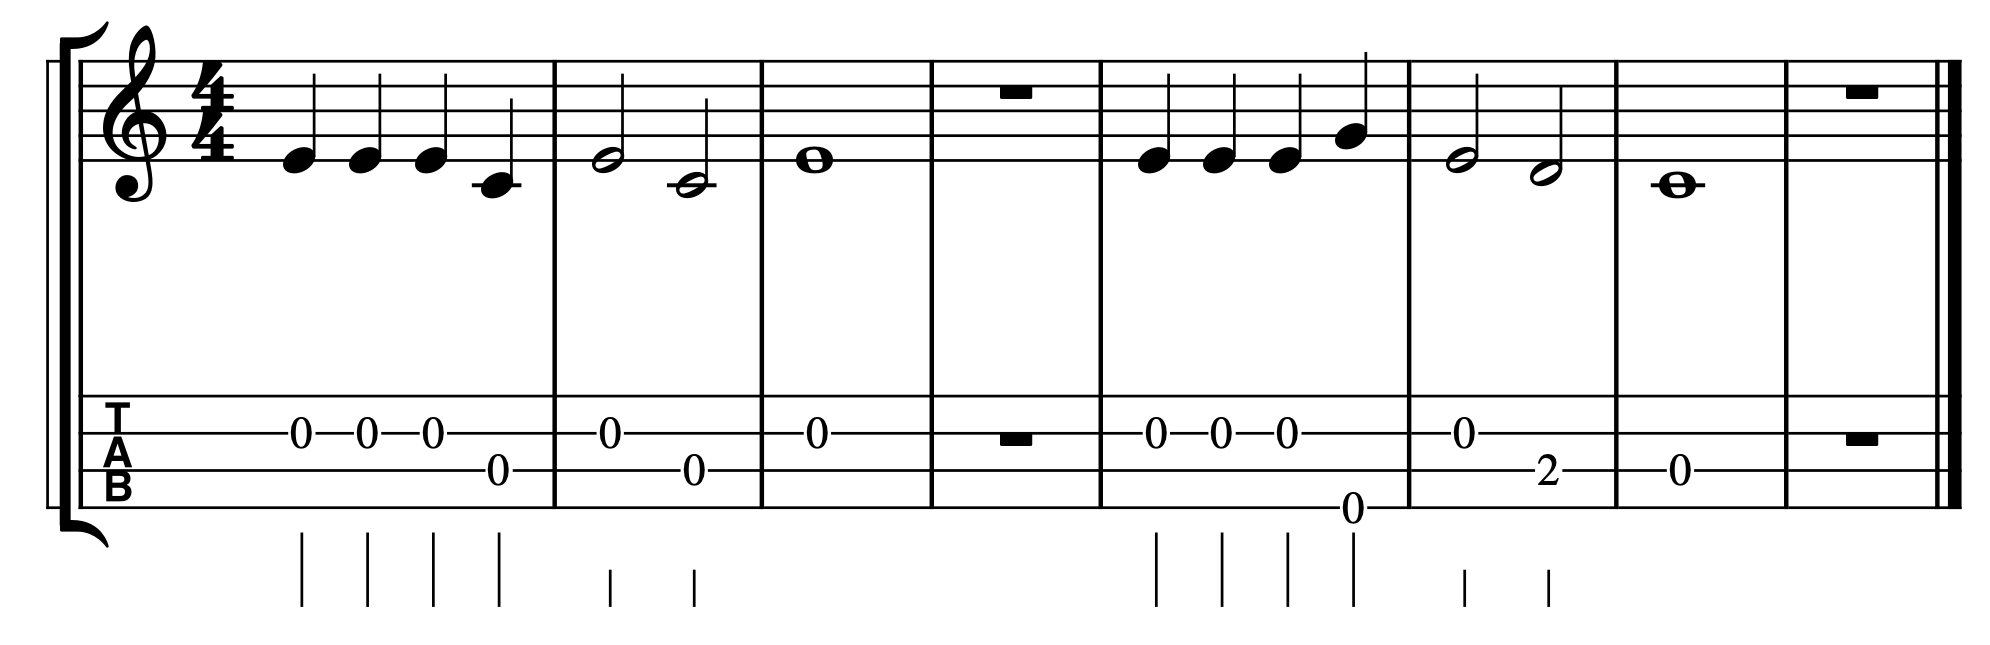
\includegraphics[width=0.9\textwidth]{little_talks_tab.png}

\endgroup

\newpage

\begingroup % Original formatting is reset back with \endgroup

\large

\section*{Najpoužívanejšie akordy}

Akordy bližšie stredu sú používané častejšie.

\bigskip
\bigskip

\begin{centering}
\ukechord{Gm} \qquad
\ukechord{Dm} \qquad
\ukechord{Am} \qquad
\ukechord{Em} \qquad
\ukechord{Bm} \qquad
\ukechord{Fsharpm}
\bigskip

\ukechord{Bb} \qquad
\ukechord{F} \qquad
\ukechord{C} \qquad
\ukechord{G} \qquad
\ukechord{D} \qquad
\ukechord{A}

\bigskip

\ukechord{F7} \qquad
\ukechord{C7} \qquad
\ukechord{G7} \qquad
\ukechord{D7} \qquad
\ukechord{A7} \qquad
\ukechord{E7}

\end{centering}

\endgroup



\end{document}
